%%%---PREAMBLE---%%%%%%%%%%%%%%%%%%%%%%%%%%%%
\documentclass[proquest,12pt,final]{ucthesis-CA2012} % change this for oneside, twoside, 11pt, draft, etc.

% fix for pandoc 1.14
\providecommand{\tightlist}{%
  \setlength{\itemsep}{0pt}\setlength{\parskip}{0pt}}

%--- Packages --------------------------------------------------------
\usepackage[lofdepth,lotdepth,caption=false]{subfig}
\usepackage{fancyhdr}
\usepackage{amsmath, amssymb, graphicx}
\usepackage{xspace}
\usepackage{braket}
\usepackage{color}
\usepackage{setspace}
\usepackage{fancyvrb}
\usepackage{array}
\usepackage{ifxetex,ifluatex}
\usepackage{etoolbox}

%% for the per mil symbol
\usepackage[nointegrals]{wasysym}

%% for more attractive tables
\usepackage{booktabs}
\usepackage{xcolor}
\usepackage{longtable}
\usepackage{lscape}
\usepackage{tabularx}

\usepackage[nostamp]{draftwatermark}
% % Use the following to make modification
\SetWatermarkText{DRAFT}
\SetWatermarkLightness{0.95}

% suppress bottom page numbers on 1st page of each chapt.
% because they overlap with text
%\patchcmd{\chapter}{plain}{empty}{}{} % turn off for UCD requirements of page number on every page

%---New Definitions and Commands------------------------------------------------------

\newtheorem{theorem}{Jibberish}

\bibliography{references}

\hyphenation{mar-gin-al-ia}

% from uw_template.tex

% commands and environments needed by pandoc snippets
% extracted from the output of `pandoc -s`
%% Make R markdown code chunks work

\ifxetex
  \usepackage{fontspec,xltxtra,xunicode}
  \defaultfontfeatures{Mapping=tex-text,Scale=MatchLowercase}
\else
  \ifluatex
    \usepackage{fontspec}
    \defaultfontfeatures{Mapping=tex-text,Scale=MatchLowercase}
  \else
    \usepackage[utf8]{inputenc}
  \fi
\fi
\DefineShortVerb[commandchars=\\\{\}]{\|}
\DefineVerbatimEnvironment{Highlighting}{Verbatim}{commandchars=\\\{\}}
% Add ',fontsize=\small' for more characters per line
\newenvironment{Shaded}{}{}
\newcommand{\KeywordTok}[1]{\textcolor[rgb]{0.00,0.44,0.13}{\textbf{{#1}}}}
\newcommand{\DataTypeTok}[1]{\textcolor[rgb]{0.56,0.13,0.00}{{#1}}}
\newcommand{\DecValTok}[1]{\textcolor[rgb]{0.25,0.63,0.44}{{#1}}}
\newcommand{\BaseNTok}[1]{\textcolor[rgb]{0.25,0.63,0.44}{{#1}}}
\newcommand{\FloatTok}[1]{\textcolor[rgb]{0.25,0.63,0.44}{{#1}}}
\newcommand{\CharTok}[1]{\textcolor[rgb]{0.25,0.44,0.63}{{#1}}}
\newcommand{\StringTok}[1]{\textcolor[rgb]{0.25,0.44,0.63}{{#1}}}
\newcommand{\CommentTok}[1]{\textcolor[rgb]{0.38,0.63,0.69}{\textit{{#1}}}}
\newcommand{\OtherTok}[1]{\textcolor[rgb]{0.00,0.44,0.13}{{#1}}}
\newcommand{\AlertTok}[1]{\textcolor[rgb]{1.00,0.00,0.00}{\textbf{{#1}}}}
\newcommand{\FunctionTok}[1]{\textcolor[rgb]{0.02,0.16,0.49}{{#1}}}
\newcommand{\RegionMarkerTok}[1]{{#1}}
\newcommand{\ErrorTok}[1]{\textcolor[rgb]{1.00,0.00,0.00}{\textbf{{#1}}}}
\newcommand{\NormalTok}[1]{{#1}}
\newcommand{\OperatorTok}[1]{\textcolor[rgb]{0.00,0.44,0.13}{\textbf{{#1}}}}
\newcommand{\BuiltInTok}[1]{\textcolor[rgb]{0.00,0.44,0.13}{\textbf{{#1}}}}
\newcommand{\ControlFlowTok}[1]{\textcolor[rgb]{0.00,0.44,0.13}{\textbf{{#1}}}}

\ifxetex
  \usepackage[setpagesize=false, % page size defined by xetex
              unicode=false, % unicode breaks when used with xetex
              xetex,
              colorlinks=true,
              linkcolor=blue]{hyperref}
\else
  \usepackage[unicode=true,
              colorlinks=true,
              linkcolor=blue]{hyperref}
\fi
\hypersetup{breaklinks=true, pdfborder={0 0 0}}
\setlength{\parindent}{0pt}
\setlength{\parskip}{6pt plus 2pt minus 1pt}
\setlength{\emergencystretch}{3em}  % prevent overfull lines
\setcounter{secnumdepth}{0}

%---Set Margins ------------------------------------------------------
\setlength\oddsidemargin{0.25 in} \setlength\evensidemargin{0.25 in} \setlength\textwidth{6.25 in} \setlength\textheight{8.5 in} %8.5
\setlength\footskip{0.25 in} \setlength\topmargin{0 in} \setlength\headheight{0.25 in} \setlength\headsep{0.25 in}

%%%---DOCUMENT---%%%%%%%%%%%%%%%%%%%%%%%%%%%%
\begin{document}


%=== Preliminary Pages ============================================
\begin{ucfrontmatter}

  %%%%%%%%%%%%%%%%%%%%%%%%%%%
  % TITLE PAGE INFORMATION % % modified to meet UCDavis
  %%%%%%%%%%%%%%%%%%%%%%%%%%%

  \title{Population genetics of a sentinel stream-breeding frog (\emph{Rana
boylii})}
  \author{Ryan A Peek}
  % \prevdegreeA{B.S. (University of California, Davis) 2002}
  % \prevdegreeB{M.S. (University of San Francisco) 2010}
  \report{DISSERTATION} 
  \degree{DOCTOR OF PHILOSOPHY} 
  \degreemonth{December} \degreeyear{2018}
  \chair{Michael R. Miller}  % this is your advisor
  \othermemberA{Peter B. Moyle} % This is a member of your committee
  \othermemberB{Mark W. Schwartz} % This is a member of your committee
  \othermemberC{} % This is a member of your committee
  \numberofmembers{3} % should match the number of entries above (chair + othermembers)
  \field{Ecology}
  \campus{Davis}
	
  % MAKE THE TITLE PAGE
	\maketitle
	
	% MAKE THE APPROVAL SHEET
	% \approvalpage

  % COPYRIGHT
  % \copyrightpage % if you want
  
  % DEDICATION %
  %%%%%%%%%%%%%%%%%%%%
    \begin{dedication}

      \vspace*{20ex} % was 25
      \begin{center}
      \begin{large} % was Large

        ``\emph{The good life of any river may depend on the perception of its
        music; and the preservation of some music to perceive.}''\\
        (Aldo Leopold)
        \begin{quote}
        ``\emph{One thing to remember is to talk to the animals. If you do, they
        will talk back to you. But if you don't talk to them, they won't talk
        back to you, then you won't understand. And when you don't understand,
        you will fear, and when you fear, you will destroy the animals, and if
        you destroy the animals, you will destroy yourself}''\\
        (Chief Dan George, Tseil-Waututh Nation, North Vancouver)
        \end{quote}
      \end{large}
      \end{center}
  \end{dedication}
  % ACKNOWLEDGEMENTS %
  %%%%%%%%%%%%%%%%%%%%
  \begin{acknowledgements}
    For all the curious people who have come before and hopefully after, I
    want to acknowledge you, and I hope we can do better to inspire and
    support those voices that may not have had the opportunities or
    priviledge I have had. I am lucky to have had all I have had, and
    finishing a dissertation requires a community, and this dissertation
    would not have happened if it wasn't for the amazing community of
    family, friends, and colleagues who helped me every step of the way. In
    particular, thank you to my partner, wife and best-friend Leslie---you
    are my sun and gravity---you held me together, anchored our family, and
    made it possible to run this crazy academic ultra-marathon. To my
    dearest little tadpoles, Connor and Genevieve, you inspire me, you make
    me laugh every day, and you remind me the world still has hope as long
    as we nourish joy and curiosity. Thank you for being you, and I hope one
    day you forgive me for the amount of time I've spent staring at a
    computer. Thanks to my mom for all the support, love, and baked goods.
    Sibling, thank you for consistently inspiring me, listening to me, and
    being the best sibling one could ask for. And for all my close friends,
    bandmates, and officemates (you know who you are), you keep me sane, you
    motivate me, and you remind me every day that I really love this crazy
    journey. John, your shed and couch have probably single-handedly kept me
    anchored in ways I can't even express\ldots{}also your friendship. Thank
    you for your time, humor, and general levity. Thanks to my Dad, who has
    cajoled, pestered, and annoyed me for far too long to ``get a PhD'',
    thanks for believing it was possible even when I didn't. Also, please
    never suggest anything like this again. And to my committee and my
    colleagues at the Center for Watershed Sciences, you have all been an
    amazing resource in providing feedback, guidance, and support throughout
    my graduate student career. Finally, to my cohort and fellow students in
    the GGE, this has been a great place to grow and mature as a scientist
    and researcher. Thank you all.
  \end{acknowledgements}
  % removed CV section from this but see gauchodown or huskydown

  % ABSTRACT %
  %%%%%%%%%%%%%%%%%%%%%%%%%%%
  \begin{abstract}
    \addcontentsline{toc}{chapter}{Abstract}

    \emph{Rana boylii} is an imperiled frog species native to CA and OR, and
    it is currently designated as a species of special concern in the state
    of CA. It has been petitioned as candidate for federal (USFWS) and state
    (CDFW) listing. As a lotic breeding amphibian, \emph{R. boylii} is tied
    closely to local flow regimes in the watersheds it inhabits and is
    therefore particularly sensitive to alterations to the natural flow
    regime. Effective conservation management of this species should
    consider and prioritize maintenance of genetic diversity as part of any
    listing decision because it is closely related to the evolutionary
    capacity for adaptation to environmental change. Conservation of genetic
    diversity in this species will require several components, including
    refining potential conservation units (i.e., distinct population
    segments) and quantifying of genetic diversity and genetic diversity
    trajectories across the species range. To assess these components,
    fine-scale and landscape-scale analyses were conducted using genomic
    data from over 600 samples from 89 localities across the range of the
    species. Six genomically-distinct groups were identified, as well as
    population subdivisions at local watershed scales. One major impact on
    \emph{R. boylii} populations has been river regulation. River regulation
    has been implicated as a cause of fundamental changes to downstream
    aquatic ecosystems. Regulation changes the natural flow regime which may
    restrict population connectivity and decrease genetic diversity in some
    species. Since population connectivity and the maintenance of genetic
    diversity are fundamental drivers of long-term persistence,
    understanding the extent that river regulation impacts these critical
    attributes of genetic health is an important goal. However, the extent
    to which \emph{R. boylii} populations in regulated rivers have
    maintained connectivity and genetic diversity is unknown. The impacts of
    river regulation on \emph{R. boylii} were investigated with genomic data
    to explore the potential for long-term persistence of \emph{R. boylii}
    under continued regulation. \emph{R. boylii} in regulated rivers showed
    striking patterns of isolation and trajectories of genetic diversity
    loss relative to unregulated rivers. For example, river regulation
    explained the greatest amount of variance in population genetic
    differentiation compared with other covariates including geographic
    distance. Importantly, patterns of connectivity and genetic diversity
    loss were observed regardless of regulation level but were most
    prominent in locations with the greatest regulation intensity. Using the
    same genomic data, fine-scale analyses of \emph{R. boylii} and \emph{R.
    sierrae} in a single region of the Sierra Nevada of California was
    conducted to evaluate the potential for hybridization between species.
    Hybridization between species may combine parental genotypes in ways
    that yield reproductively sterile or isolated lineages, and
    hybridization events may be short-lived and difficult to detect. Limited
    hybridization between the species was detected in the Feather basin,
    though it appears these are terminal events based on PCA, admixture, and
    tests of heterozygosity using species diagnostic SNPs. Finally,
    rangewide quantification and comparison of genomic variation across
    populations indicates the southern coast, southern Sierra Nevada, and
    Northern Sierra/Feather basin in California should have high
    prioritization in conservation efforts due to low genomic diversity and
    trajectories of diversity loss. More broadly, these results demonstrate
    both the critical need for regional conservation in a sentinel river
    species, and the utility and power of genetic methods for assessing and
    monitoring sensitive species across many scales.

    %\abstractsignature
  \end{abstract}
  % Table of Contents %
  %%%%%%%%%%%%%%%%%%%%%%%%%%%
	\tableofcontents

\end{ucfrontmatter} % end of the preliminary pages
\begin{ucmainmatter}

\hypertarget{reg-health}{%
\chapter{Flow regulation associated with decreased genetic health of a
river-breeding frog species}\label{reg-health}}

\hypertarget{introduction}{%
\section{Introduction}\label{introduction}}

Rivers simultaneously connect and carve the landscapes through which
they flow. Rivers provide corridors of connectivity for riparian and
aquatic organisms such as fish, amphibians, and macroinvertebrates
(Wiens \protect\hyperlink{ref-wiens_riverine_2002}{2002}, Pringle
\protect\hyperlink{ref-pringle_what_2003}{2003}), while also acting as
physical barriers on the landscape for many terrestrial organisms
(Voelker et al. \protect\hyperlink{ref-voelker_river_2013}{2013}, Cazé
et al. \protect\hyperlink{ref-caze_could_2016}{2016}). Hydrologic
connectivity (Pringle \protect\hyperlink{ref-pringle_what_2003}{2003})
transfers energy, organisms and ultimately genetic variation and thus is
a critical component for population persistence in dynamic systems where
populations must constantly adapt to temporal and spatial changes. In
Mediterranean climates, rivers have strong seasonal patterns associated
with cold, wet winters and warm, dry summers. Native aquatic organisms
have evolved life histories well adapted to these natural patterns,
which are both predictable and seasonal (Yarnell et al.
\protect\hyperlink{ref-yarnell_ecology_2010}{2010}, Tonkin et al.
\protect\hyperlink{ref-tonkin_seasonality_2017}{2017}).

River regulation, or the hydrological alteration of flow by dams and
diversions, impacts the seasonal and interannual flow variability within
a watershed. Regulation changes the natural flow regime and dramatically
alters geomorphic and hydrologic connectivity of watersheds (Poff et al.
\protect\hyperlink{ref-poff_homogenization_2007}{2007}), which may
restrict natural population connectivity (Schick and Lindley
\protect\hyperlink{ref-schick_directed_2007}{2007}, Shaw et al.
\protect\hyperlink{ref-shaw_importance_2016}{2016}). River regulation
can change flow frequency, magnitude, duration, timing, and rate of
change, which can have significant impacts on aquatic organisms and
ecological processes (Poff et al.
\protect\hyperlink{ref-poff_homogenization_2007}{2007}, Yarnell et al.
\protect\hyperlink{ref-yarnell_ecology_2010}{2010}). River regulation,
and more specifically, regulation associated with hydropower generation,
has been implicated as a cause of fundamental changes to downstream
aquatic ecosystems (Power et al.
\protect\hyperlink{ref-power_dams_1996}{1996}, Bunn and Arthington
\protect\hyperlink{ref-bunn_basic_2002}{2002}, Moyle et al.
\protect\hyperlink{ref-moyle_rapid_2011}{2011}). The hydrological
regimes of over half of the world's largest rivers have been altered by
large dams (Nilsson et al.
\protect\hyperlink{ref-nilsson_fragmentation_2005}{2005}) and only
recently has the extent of flow alteration and the associated
ecosystem-level impacts been acknowledged (Pringle
\protect\hyperlink{ref-pringle_hydrologic_2001}{2001}, Dudgeon et al.
\protect\hyperlink{ref-dudgeon_freshwater_2006}{2006}, Murchie et al.
\protect\hyperlink{ref-murchie_fish_2008}{2008}).

Changes to abiotic processes caused by river regulation can have a
substantial impact on biotic communities. The negative effects of river
regulation on migration and loss of spawning habitat (Lind et al.
\protect\hyperlink{ref-lind_effects_1996}{1996}, Fuller et al.
\protect\hyperlink{ref-fuller_linking_2011}{2011}, Kupferberg et al.
\protect\hyperlink{ref-kupferberg_effects_2012}{2012}, Rolls and Bond
\protect\hyperlink{ref-rolls_environmental_2017}{2017}), reductions in
population abundances and diversity (Zhong and Power
\protect\hyperlink{ref-zhong_environmental_1996}{1996}, Vorosmarty et
al. \protect\hyperlink{ref-vorosmarty_global_2010}{2010}, Fuller et al.
\protect\hyperlink{ref-fuller_linking_2011}{2011}, Werth et al.
\protect\hyperlink{ref-werth_dams_2014}{2014}, Scribner et al.
\protect\hyperlink{ref-scribner_applications_2016}{2016}, Sabo et al.
\protect\hyperlink{ref-sabo_designing_2017}{2017}, Guzy et al.
\protect\hyperlink{ref-guzy_influence_2018}{2018}), and fragmentation
(Vorosmarty et al. \protect\hyperlink{ref-vorosmarty_global_2010}{2010},
Werth et al. \protect\hyperlink{ref-werth_dams_2014}{2014}, Scribner et
al. \protect\hyperlink{ref-scribner_applications_2016}{2016}, Sabo et
al. \protect\hyperlink{ref-sabo_designing_2017}{2017}, Guzy et al.
\protect\hyperlink{ref-guzy_influence_2018}{2018}) have been well
documented. However, most rivers have not been regulated for long
periods (e.g., less than 100 years) compared to the time these organisms
had to adapt to pre-anthropogenic river flow. In regulated rivers that
organisms still occupy, it remains unknown whether populations can
persist long-term with continued regulation. In other words, while some
species may have persisted since regulation began in a system (e.g.,
several decades), this does not necessarily mean these populations will
persist into the future under current flow regulation regimes. Thus,
exploring the potential for long-term persistence of populations under
different flow regimes is a crucial component for guiding conservation
efforts yet remains a significant gap.

One tool that can help address this gap is the integration of genetics
and hydrology to better assess the impact of river regulation on aquatic
organisms (Scribner et al.
\protect\hyperlink{ref-scribner_applications_2016}{2016}). Although
aquatic organisms are often difficult to count and monitor by
conventional methods, genetic monitoring can be a powerful tool to
assess population health by revealing factors such as fragmentation and
population declines. It is widely recognized that reductions in
population connectivity can increase isolation and inbreeding, leading
to a potential ``extinction vortex'' (Gilpin and Soule
\protect\hyperlink{ref-gilpin_minimum_1986}{1986}), yet there is limited
understanding of how flow alteration may impair the processes crucial
for maintenance of genetic variation and thus adaptive capacity. In
addition, there is a current pressing need for more effective and
flexible watershed management tools, particularly in relation to
monitoring aquatic populations and implementation of environmental flows
(Grantham et al. \protect\hyperlink{ref-grantham_climatic_2010}{2010}).
Thus, population genetics could be a powerful tool to understand the
influence of different flow regimes on population health and this
information could facilitate improved flow management to better protect
aquatic populations.

The river-breeding foothill yellow-legged frog (\emph{Rana boylii};
FYLF) historically occurred in lower and mid-elevation streams and
rivers from Southern Oregon to northern Baja California west of the
Sierra-Cascade crest (Stebbins
\protect\hyperlink{ref-stebbins_field_2003}{2003}). \emph{Rana boylii}
are intimately linked with river hydrology because they have evolved to
spawn in synchrony with natural flow cues associated with seasonal
spring snowmelt or rain recession periods (Kupferberg
\protect\hyperlink{ref-kupferberg_hydrologic_1996}{1996}, Yarnell et al.
\protect\hyperlink{ref-yarnell_ecology_2010}{2010},
\protect\hyperlink{ref-yarnell_management_2016}{2016}, Bondi et al.
\protect\hyperlink{ref-bondi_transferability_2013}{2013}). However,
population declines have been documented across the former range of this
species, particularly in southern California and the Sierra Nevada where
it has been extirpated from approximately 50 percent of its historical
range (Jennings and Hayes
\protect\hyperlink{ref-jennings_amphibian_1994}{1994}, Davidson et al.
\protect\hyperlink{ref-davidson_spatial_2002}{2002}).

\par

In California, particularly in the Sierra Nevada, river regulation may
be a significant environmental stressor (Lind et al.
\protect\hyperlink{ref-lind_effects_1996}{1996}, Kupferberg et al.
\protect\hyperlink{ref-kupferberg_effects_2012}{2012}). Regulated river
reaches typically alter flows by augmenting or diverting winter and
spring runoff, thereby reducing or eliminating flow cues and disrupting
natural flow regimes. Aseasonal flow fluctuation from river regulation
can scour (detach from substrate) or desiccate \emph{R. boylii} egg
masses, and the loss of clutches may have a significant demographic
impact because only one egg mass is laid per year. In many regulated
rivers in the Sierra Nevada, \emph{R. boylii} populations are now
restricted to small unregulated tributaries flowing into the regulated
mainstem.

\par

Here, we investigated the impacts of river regulation on genetic
diversity of \emph{R. boylii} populations across three different flow
regimes. Given that population connectivity and genetic diversity are
known to be play critical roles in long-term species persistence, we
explored the association between these metrics and levels of river
regulation. Our goal was to assess the genetic health (through metrics
of genetic diversity) of \emph{R. boylii} under different river
regulation regimes to better inform the potential for long-term
persistence. These data can be used to prioritize management and
conservation efforts for \emph{R. boylii}, as well as demonstrate the
potential utility of genetics for future conservation monitoring efforts
in aquatic species.

\hypertarget{methods}{%
\section{Methods}\label{methods}}

\hypertarget{ch1samplecollection}{%
\subsection{Sample collection and DNA
extraction}\label{ch1samplecollection}}

345 \emph{R. boylii} buccal or tissue samples were used in this study
across six different rivers (Table \ref{tab:CH1T1},
\protect\hyperlink{supptables}{Appendix, S1}). Field sampling was
conducted following Heyer et al.
(\protect\hyperlink{ref-heyer_measuring_1994}{1994}), under CDFW SCP
Permit \#0006881, with IACUC protocol \#19327. Individual
post-metamorphic frogs were buccal-swabbed following established
protocols (Goldberg et al.
\protect\hyperlink{ref-goldberg_frogs_2003}{2003}, Pidancier et al.
\protect\hyperlink{ref-pidancier_buccal_2003}{2003}, Broquet et al.
\protect\hyperlink{ref-broquet_buccal_2007}{2007}). Each
post-metamorphic individual was comprehensively swabbed underneath
tongue and cheek for approximately one minute. Swabs were air dried for
approximately five minutes and placed in 1.5 mL microcentrifuge tubes
while in the field. Samples were stored in the laboratory at -80°C until
DNA extraction. Where possible, tail clips from tadpole larvae were
collected, and tadpoles greater than 15 mm total length were targeted
(Wilbur and Semlitsch
\protect\hyperlink{ref-wilbur_ecological_1990}{1990}, Parris et al.
\protect\hyperlink{ref-parris_assessing_2010}{2010}). One small
(\textless{}3mm) tail clip was taken per individual tadpole and dried on
Whatman qualitative filter paper (grade 1) and stored at room
temperature. Some older tissue samples consisted of toe clips placed in
100\% ethanol for storage, and DNA extraction from these samples used
Qiagen DNeasy kits following the manufacturer's protocol. Buccal swabs
and tail clip DNA were extracted with a magnetic bead--based protocol
(Ali et al. \protect\hyperlink{ref-ali_rad_2016}{2016}) and quantified
using Quant-iT PicoGreen dsDNA Reagent (Thermo Fisher Scientific) with
an FLx800 Fluorescence Reader (BioTek Instruments).
\begin{landscape}\begin{table}

\caption{\label{tab:CH1T1}Sampling and locality information for population genomic analysis in the Yuba, Bear, and American watersheds in the northern Sierra Nevada of California, USA. The number of individuals (n) is given for the total number sequenced per location and the number of individuals that were retained after filtering across the 8,533 baits. NHD refers to the National Hydrography Dataset by USGS (U.S. Geological Survey, National Hydrography Dataset, Digital data, accessed, August 2017).}
\centering
\resizebox{\linewidth}{!}{
\begin{tabular}[t]{lrllllrrrrrrr}
\toprule
Site Name & SiteID & Locality & River & Watershed & Regulation Type & Lat. & Lon. & Elev. (m) & NHD Stream Order & NHD Total Drainage Area (sq. km) & n initial & n retained\\
\midrule
BEAR & 20 & Chicago Powerhouse & Bear & Bear & Bypass & 39.17484 & -120.8998 & 665.7990 & 4 & 136.0 & 6 & 6\\
BEAR\_GRHN & 16 & Greenhorn Creek & Bear & Bear & Bypass & 39.23206 & -120.9019 & 820.5347 & 2 & 11.0 & 15 & 6\\
BEAR\_STH2 & 19 & Steep Hollow Creek US & Bear & Bear & Bypass & 39.19444 & -120.8878 & 704.6578 & 2 & 45.0 & 7 & 6\\
BEAR\_STHA & 18 & Hawkins Ravine & Bear & Bear & Bypass & 39.18833 & -120.8981 & 706.9961 & 2 & 4.0 & 3 & 3\\
BEAR\_STHC & 17 & Steep Hollow Creek DS & Bear & Bear & Bypass & 39.20231 & -120.8754 & 736.8513 & 2 & 52.0 & 13 & 12\\
\addlinespace
MFA\_AMEC & 1 & American Canyon & MF American & American & Hydropeaking & 38.93396 & -120.9436 & 240.3928 & 2 & 9.0 & 16 & 6\\
MFA\_GASC & 2 & Gas Canyon & MF American & American & Hydropeaking & 38.96651 & -120.9325 & 241.8506 & 1 & 13.0 & 6 & 6\\
MFA\_TODC & 3 & Todd Creek & MF American & American & Hydropeaking & 38.96385 & -120.9216 & 367.7263 & 2 & 10.0 & 11 & 9\\
MFY\_OREGCK & 27 & Oregon Creek & Middle Yuba & Yuba & Bypass & 39.44188 & -121.0575 & 620.4250 & 4 & 375.0 & 15 & 13\\
MFY\_US\_OH & 28 & US Our House Dam & Middle Yuba & Yuba & Bypass & 39.41305 & -120.9903 & 624.1467 & 4 & 375.0 & 13 & 12\\
\addlinespace
NFA & 13 & Iowa Hill Mainstem & NF American & American & Unregulated & 39.11115 & -120.9168 & 386.4710 & 4 & 605.0 & 36 & 30\\
NFA\_BUNC & 8 & Bunch Canyon & NF American & American & Unregulated & 39.03762 & -120.9103 & 286.2874 & 3 & 27.0 & 15 & 14\\
NFA\_EUCH & 14 & Euchre Bar & NF American & American & Unregulated & 39.18492 & -120.7620 & 579.5186 & 4 & 508.0 & 13 & 11\\
NFA\_INDC & 10 & Indian Creek & NF American & American & Unregulated & 39.05665 & -120.9085 & 296.1071 & 2 & 24.0 & 12 & 11\\
NFA\_POND & 7 & Ponderosa Bridge & NF American & American & Unregulated & 38.99995 & -120.9406 & 240.8255 & 5 & 857.0 & 5 & 5\\
\addlinespace
NFA\_ROBR & 12 & Robbers Ravine & NF American & American & Unregulated & 39.10451 & -120.9267 & 400.0005 & 1 & 4.0 & 30 & 11\\
NFA\_SAIC & 15 & Sailor Canyon & NF American & American & Unregulated & 39.21694 & -120.4960 & 1005.5781 & 3 & 166.0 & 8 & 5\\
NFA\_SHIC & 9 & Shirttail Creek & NF American & American & Unregulated & 39.04446 & -120.8994 & 525.7589 & 4 & 141.0 & 16 & 15\\
NFA\_SLAR & 11 & Slaughter Ravine & NF American & American & Unregulated & 39.09865 & -120.9255 & 356.0791 & 2 & 6.0 & 8 & 8\\
NFMFA\_SC & 4 & NFMFA-Skunk Canyon & MF American & American & Hydropeaking & 39.02237 & -120.7369 & 521.5720 & 2 & 6.0 & 18 & 18\\
\addlinespace
NFY & 29 & Rocky Rest Mainstem & North Yuba & Yuba & Unregulated & 39.51190 & -120.9774 & 704.6863 & 5 & 669.0 & 15 & 12\\
NFY\_SLATE\_CGRAV & 30 & Slate Creek & North Yuba & Yuba & Bypass & 39.68913 & -120.9389 & 1330.9373 & 3 & 58.7 & 4 & 4\\
RUB\_LCUS & 6 & Rubicon-Long Canyon & MF American & American & Bypass & 38.98887 & -120.6900 & 415.1026 & 5 & 806.0 & 9 & 8\\
RUB\_USPH & 5 & Rubicon-US Powerhouse & MF American & American & Bypass & 38.99928 & -120.7233 & 360.5759 & 5 & 816.0 & 11 & 11\\
SFY & 26 & US Canyon Creek & South Yuba & Yuba & Bypass & 39.35386 & -120.7342 & 889.7745 & 4 & 365.0 & 6 & 6\\
\addlinespace
SFY\_LOGA & 25 & Logan Creek & South Yuba & Yuba & Bypass & 39.36914 & -120.8526 & 1201.1790 & 1 & 5.0 & 5 & 4\\
SFY\_MISC & 24 & Missouri Canyon & South Yuba & Yuba & Bypass & 39.36096 & -120.8814 & 1094.6312 & 2 & 5.0 & 8 & 6\\
SFY\_ROCKCK & 23 & Rock Creek & South Yuba & Yuba & Bypass & 39.32983 & -120.9863 & 593.5214 & 4 & 710.0 & 3 & 3\\
SFY\_SHADYCK & 21 & Shady Creek & South Yuba & Yuba & Bypass & 39.35433 & -121.0590 & 675.0255 & 2 & 15.0 & 14 & 12\\
SFY\_SPRINGCK & 22 & Spring Creek & South Yuba & Yuba & Bypass & 39.33233 & -120.9890 & 595.1054 & 3 & 24.0 & 4 & 4\\
\bottomrule
\end{tabular}}
\end{table}
\end{landscape}
\hypertarget{denovo}{%
\subsection{Sequencing and de novo assembly}\label{denovo}}

To produce a high-quality genomic resource for a frog species with a
large genome size, we first interrogated a large fraction of the genome
using a SbfI restriction enzyme and high-density RAD sequencing on an
Illumina HiSeq (Miller et al.
\protect\hyperlink{ref-miller_rapid_2007}{2007}, Baird et al.
\protect\hyperlink{ref-baird_rapid_2008}{2008}). Paired-end sequence
data were generated from 24 \emph{R. boylii} individuals collected
previously (Peek \protect\hyperlink{ref-peek_landscape_2010}{2010}) from
coastal and Sierra Nevada populations in California, USA
\protect\hyperlink{supptables}{(Appendix, S2)}. RAD libraries were
constructed following the protocol described in Ali et al.
(\protect\hyperlink{ref-ali_rad_2016}{2016}). \emph{De novo} loci
discovery and contig extension were carried via custom PERL scripts
(Miller et al. \protect\hyperlink{ref-miller_conserved_2012}{2012})
using the alignment program Novoalign and the genome assembler PRICE
(Ruby et al. \protect\hyperlink{ref-ruby_price_2013}{2013}). This
pipeline resulted in a set of 77,544 RAD contigs ranging from 300 to 800
bp which served as a \emph{de novo} partial genome reference for all
subsequent downstream analyses \protect\hyperlink{supptables}{(Appendix,
S3)}. Using these data, we filtered data to loci with 4 or fewer SNPs,
and randomly selected 10,000 loci from this subset. Using these RADSeq
data, 8,533 RAD capture baits (120bp) were designed by Arbor Biosciences
from the de novo alignment \protect\hyperlink{supptables}{(Appendix,
S4)}.

\hypertarget{rapture}{%
\subsection{Rapture sequencing}\label{rapture}}

We then performed Rapture on all study samples to identify putative
high-quality SNPs \protect\hyperlink{supptables}{(Appendix, S1)} using
RAD capture baits. Three different sequencing runs on an Illumina HiSeq
were merged together, filtered, and duplicates were removed using ANGSD
and Samtools (Li et al. \protect\hyperlink{ref-li_sequence_2009}{2009}).
Sampled individuals were aligned against the de novo partial genome
reference using the BWA-MEM algorithm (Li and Durbin
\protect\hyperlink{ref-li_fast_2010}{2010}, Li
\protect\hyperlink{ref-li_aligning_2013}{2013}) and saved to BAM format.
SAMtools was used to sort, filter for proper pairs, remove PCR
duplicates, and index binary alignment map (BAM), as well as merge
sequences from multiple libraries (Li et al.
\protect\hyperlink{ref-li_sequence_2009}{2009}).

\hypertarget{principal-component-analysis}{%
\subsection{Principal component
analysis}\label{principal-component-analysis}}

A probabilistic framework was used to discover SNPs for PCA as it does
not require calling genotypes and is suitable for low-coverage
sequencing data (Korneliussen et al.
\protect\hyperlink{ref-korneliussen_calculation_2013}{2013}, Fumagalli
et al. \protect\hyperlink{ref-fumagalli_quantifying_2013}{2013}). All
Rapture analyses were conducted using Analysis of Next Generation
Sequencing Data (ANGSD) (Korneliussen et al.
\protect\hyperlink{ref-korneliussen_angsd_2014}{2014}). ANGSD analyses
were conducted following methods from Prince et al.
(\protect\hyperlink{ref-prince_evolutionary_2017}{2017}), with a minimum
mapping quality score (\texttt{minMapQ}) of 10, a minimum base quality
score (\texttt{minQ}) of 20, and the genotype likelihood model
(\texttt{GL\ 1}) (Li \protect\hyperlink{ref-li_statistical_2011}{2011}).
To maximize data quality, samples with less than 100,000 aligned reads
were excluded \protect\hyperlink{supptables}{(Appendix, S1)} and only
sites represented in at least 50\% of the included samples
(\texttt{minInd}) were used. Settings used in ANGSD for PCA to identify
polymorphic sites included a \texttt{SNP\_pval} of
1e\textsuperscript{-6}, inferring major and minor alleles
(\texttt{doMajorMinor\ 1}), estimating allele frequencies
(\texttt{doMaf\ 2}) (Kim et al.
\protect\hyperlink{ref-kim_estimation_2011}{2011}), retaining SNPs with
a minor allele frequency of at least 0.05 \texttt{(minMaf}), genotype
posterior probabilities calculated with a uniform prior
(\texttt{doPost\ 2}), and the \texttt{doIBS\ 1} and \texttt{doCov\ 1}
options were used to generate PCA data. Principal components (PC)
summarizing population structure were derived from classic eigenvalue
decomposition and were visualized using the ggplot2 package in R (R Core
Team \protect\hyperlink{ref-r_core_team_r_2017}{2017}).

\hypertarget{genetic-differentiation-and-diversity-estimates}{%
\subsection{Genetic differentiation and diversity
estimates}\label{genetic-differentiation-and-diversity-estimates}}

Mean scaled F\textsubscript{ST} was used to quantify genetic
differentiation between populations (Wright
\protect\hyperlink{ref-wright_isolation_1943}{1943}, Rousset
\protect\hyperlink{ref-rousset_genetic_1997}{1997}). Genome-wide
F\textsubscript{ST} between population pairs was estimated by first
calculating a site frequency spectrum (SFS) for each population
(\texttt{doSaf}) (Nielsen et al.
\protect\hyperlink{ref-nielsen_snp_2012}{2012}) with ANGSD. The
two-dimensional SFS and global F\textsubscript{ST} between each
population pair were then estimated using realSFS (Korneliussen et al.
\protect\hyperlink{ref-korneliussen_angsd_2014}{2014}).
F\textsubscript{ST} was calculated between each pair of collection
locations within a watershed, and the mean of all pairwise calculations
within that watershed was calculated for each location. We calculated
the river distances (distance along river network) between locations
within watersheds using the riverdist package in R (Tyers
\protect\hyperlink{ref-tyers_riverdist_2017}{2017}), and used the mean
pairwise river distance (km) to all other locations within the
watershed. These values were plotted and a generalized linear model was
fitted (\(F_{ST}\) \textasciitilde{} \(Mean River Distance\)) in R (R
Core Team \protect\hyperlink{ref-r_core_team_r_2017}{2017}). To
calculate Watterson's \(\theta\) (\(\theta_S\)) (Watterson
\protect\hyperlink{ref-watterson_number_1975}{1975}), and Tajima's
\(\theta\) (\(\theta_\pi\)) (Tajima
\protect\hyperlink{ref-tajima_evolutionary_1983}{1983}), we used SFS
that were estimated as described above as priors (\texttt{pest}) to
calculate each statistic for each site (\texttt{doThetas}), and then
averaged to obtain a single value for each statistic (Korneliussen et
al. \protect\hyperlink{ref-korneliussen_calculation_2013}{2013}).

\hypertarget{boosted-regression-tree-modeling-of-variance-in-fst}{%
\subsection{\texorpdfstring{Boosted regression tree modeling of variance
in
F\textsubscript{ST}}{Boosted regression tree modeling of variance in FST}}\label{boosted-regression-tree-modeling-of-variance-in-fst}}

We used boosted regression tree (BRT) models with the R packages gbm
(Ridgeway \protect\hyperlink{ref-ridgeway_gbm_2015}{2015}) and dismo
(Hijmans et al. \protect\hyperlink{ref-hijmans_dismo_2017}{2017}) to
assess the relative influence of river regulation as compared to other
covariates. Boosted regression trees (BRT) are suitable frameworks for
large and complex ecological datasets because they do not assume
normality, nor linear relationships between predictor and response
variables and they ignore non-informative predictor variables (Graham et
al. \protect\hyperlink{ref-graham_influence_2008}{2008}, Steel et al.
\protect\hyperlink{ref-steel_associating_2017}{2017}). BRTs use
iterative boosting algorithms to combine simple decision trees to
improve model performance (De'ath
\protect\hyperlink{ref-death_boosted_2007}{2007}) and provide a robust
alternative to many traditional statistical methods (Phillips et al.
\protect\hyperlink{ref-phillips_maximum_2006}{2006}, Guisan et al.
\protect\hyperlink{ref-guisan_what_2007}{2007}). BRTs assess the
relative impact of modeled variables by calculating the number of times
a variable is selected for splitting a tree across all folds of the
cross validation. Following Steel et al.
(\protect\hyperlink{ref-steel_associating_2017}{2017}), estimates of
relative influence for each predictor variable were used to evaluate the
relative contribution a variable had in predicting the response. To
evaluate the relative influence of covariates on F\textsubscript{ST},
models were trained using river distance (km), elevation (m), upstream
drainage area (km2), Strahler stream order, and number of samples per
location. Stream segment data on elevation, length, slope, stream order,
and drainage area were derived from NHD Plus attributes (U.S. Geological
Survey, National Hydrography Dataset, Digital data, accessed, August
2017 at \url{http://nhd.usgs.gov/data.html}). In addition,
\(\Delta \theta\) \((\theta_\pi - \theta_S)\) was included to assess the
effect of genomic variation on F\textsubscript{ST} across regulation
types.

Model training and fitting were conducted following methods previously
described in Steel et al.
(\protect\hyperlink{ref-steel_associating_2017}{2017}). To reduce
overfitting, the learning rate (also known as the shrinking rate) was
set to 0.001. Stochastic gradient boosting was utilized to reduce
prediction error (De'ath
\protect\hyperlink{ref-death_boosted_2007}{2007}) and the fraction of
training data sampled to build each tree was 0.75, within the range as
recommended by (Brown et al.
\protect\hyperlink{ref-brown_predicting_2012}{2012}). Tree complexity
was set to three to allow for second and third order interaction
effects. The minimum number of observations required in the final nodes
of each tree was three. A ten-fold cross-validation technique allowed us
to determine the number of trees at which prediction error was minimized
using the cross-validation deviance. Model performance was evaluated
using the minimum estimated cross-validation deviance which maximized
the estimated deviance explained.

\clearpage

\hypertarget{results}{%
\section{Results}\label{results}}

\hypertarget{rapture-produces-high-quality-genomic-data-for-rana-boylii}{%
\subsection{\texorpdfstring{Rapture produces high quality genomic data
for \emph{Rana
boylii}}{Rapture produces high quality genomic data for Rana boylii}}\label{rapture-produces-high-quality-genomic-data-for-rana-boylii}}

To begin investigating the impact of river regulation on \emph{R.
boylii}, we collected frog tissue and buccal samples from 30 locations
in six rivers representing three different flow impairment levels
associated with hydropower generation. The three flow regimes assessed
were: (1) hydropeaking, where flows are pulsed on most days from late
spring through fall to provide electricity during peak-use hours and for
recreational whitewater rafting; (2) bypass, which diverts river flows
from an upstream portion of the basin to the downstream power generation
facilities; and (3) unregulated, a largely natural flow regime where no
upstream controls exist to regulate flows (Figure \ref{fig:CH1F1map}).
Flow data were obtained for each river reach using proximal USGS gaging
stations (Table \ref{tab:CH1T1}). We sampled a total of 345 \emph{R.
boylii} from sites in three major watersheds (Yuba, Bear, and American)
in the northern Sierra Nevada of California (Figure \ref{fig:CH1F1map},
Table \ref{tab:CH1T1}). The six study rivers share a similar
Mediterranean climate, underlying geology, watershed aspect
(west-slope), stream morphology (riffle-pool), and vegetative
communities, but differ in the intensity of flow regulation (Steel et
al. \protect\hyperlink{ref-steel_associating_2017}{2017}). Although
river regulation occurs in all three of the study watersheds, both the
North Yuba and North Fork (NF) American are unregulated whereas the
Middle Fork (MF) American is the only river that has a hydropeaking flow
regime (Figure \ref{fig:CH1F1map}A).
\begin{table}[!h]

\caption{\label{tab:CH1T2}Metadata for USGS gaging stations with current and historic data available for each study river}
\centering
\fontsize{11}{13}\selectfont
\begin{tabular}[t]{lllrr}
\toprule
Study Site & USGS Gage Number & Years of Record & Latitude & Longitude\\
\midrule
\addlinespace[0.3em]
\multicolumn{5}{l}{\textbf{North Yuba}}\\
\hspace{1em}North Yuba & 11413000 & 1931–Present & 39.52500 & -120.9369\\
\addlinespace[0.3em]
\multicolumn{5}{l}{\textbf{Middle Yuba}}\\
\hspace{1em}Middle Yuba & 11408550 & 1987–Present & 39.52194 & -120.5825\\
\hspace{1em}Middle Yuba & 11408700 & 1957–1966 & 39.43861 & -120.8111\\
\addlinespace[0.3em]
\multicolumn{5}{l}{\textbf{South Yuba}}\\
\hspace{1em}South Yuba & 11414250 & 1965–Present & 39.31861 & -120.6567\\
\hspace{1em}South Yuba & 11417000 & 1942–1972 & 39.36056 & -120.7706\\
\addlinespace[0.3em]
\multicolumn{5}{l}{\textbf{NF American}}\\
\hspace{1em}NF American & 11427000 & 1942–Present & 38.93611 & -121.0228\\
\addlinespace[0.3em]
\multicolumn{5}{l}{\textbf{Rubicon}}\\
\hspace{1em}Rubicon & 11433200 & 1959–1984 & 38.99250 & -120.7206\\
\hspace{1em}Rubicon & 11427765 & 1974–Present & 39.00027 & -120.7231\\
\addlinespace[0.3em]
\multicolumn{5}{l}{\textbf{MF American}}\\
\hspace{1em}MF American & 11433300 & 1958–2011 & 39.00611 & -120.7597\\
\hspace{1em}MF American & 11433500 & 1911–1986 & 38.91805 & -121.0142\\
\hspace{1em}MF American & OXB (PCWA)\textsuperscript{1} & 1997–Present & 39.00600 & -120.7600\\
\bottomrule
\multicolumn{5}{l}{\textsuperscript{1} PCWA=Placer County Water Agency, http://cdec.water.ca.gov/cdecstation2/?sta=OXB}\\
\end{tabular}
\end{table}







\begin{figure}
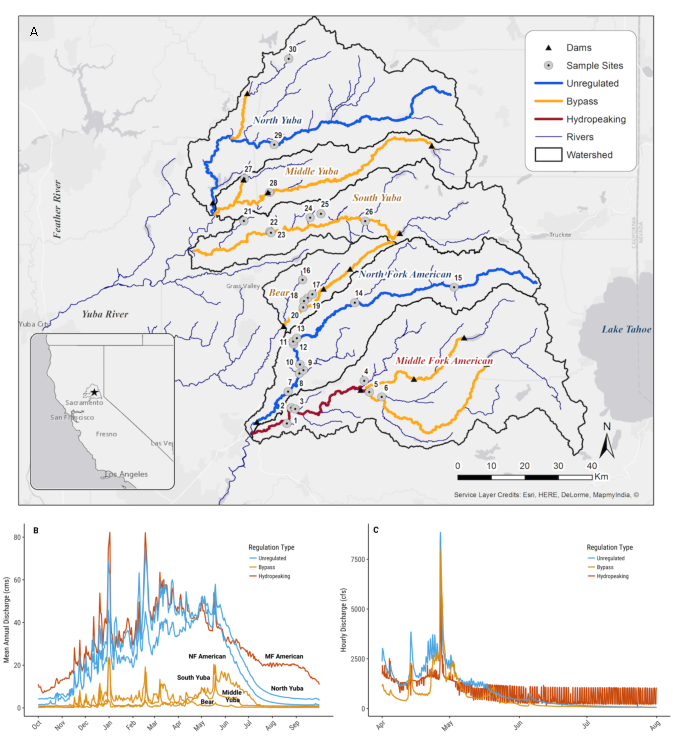
\includegraphics[width=1\linewidth]{figure/ch1/fig_01_ac_map_hydrographs} \caption{Sampling locations and flow characteristics. A) Map of
sampling locations spread across six rivers. B) Comparison of annual
mean daily discharge from 1981--2016 for three flow types. C) Comparison
of hourly discharge in three different flow regimes in April through
July 2012, Bypass (South Yuba), Hydropeaking (Middle Fork American), and
Unregulated (North Fork American). See Table \ref{tab:CH1T2} for USGS
gaging station information.}\label{fig:CH1F1map}
\end{figure}
To generate genetic data from the samples, we performed RAD Capture
(a.k.a. Rapture) (Ali et al. \protect\hyperlink{ref-ali_rad_2016}{2016})
on the samples by generating SbfI RAD libraries, capturing a subset of
the RAD loci using 8,533 baits (see Methods), and sequencing the
resulting library on an Illumina HiSeq. We then aligned the sequencing
reads from each sample to a de novo RAD assembly (see Methods). The mean
number of filtered alignments across all 345 samples was 324,928. For
downstream analysis, we selected individuals that had greater than
100,000 alignments (n=277), which provided sufficient data to
investigate population genetic attributes at broad and fine geographic
scales (see below). \emph{R. boylii} are cryptic, and often occur in low
densities within the study area. Thus, we retained a minimum of three
individuals per site, and the mean number of samples per site was
approximately nine (Table \ref{tab:CH1T1}). With genomic data,
population genetic parameters can be accurately estimated from even low
sample numbers (Hotaling et al.
\protect\hyperlink{ref-hotaling_demographic_2018}{2018}), and genomic
analyses in non-model organism often use fewer loci (Narum et al.
\protect\hyperlink{ref-narum_genotyping-by-sequencing_2013}{2013}). We
conclude that the sequence data we obtained should be appropriate for
population genetic analyses across our study area.

\hypertarget{anomalous-genetic-pattern-in-highly-regulated-reach-of-middle-fork-american-watershed}{%
\subsection{Anomalous genetic pattern in highly regulated reach of
Middle Fork American
watershed}\label{anomalous-genetic-pattern-in-highly-regulated-reach-of-middle-fork-american-watershed}}

To assess \emph{R. boylii} population structure across the collection
locations, we used ANGSD (Korneliussen et al.
\protect\hyperlink{ref-korneliussen_angsd_2014}{2014}) to discover
44,406 SNPs and perform principal component analysis (PCA; see Methods),
which provides a dimensionless comparison of all samples. The first two
principal components revealed four main groups corresponding to the
Yuba, Bear, North Fork (NF) American, and Middle Fork (MF) American
samples (Figure \ref{fig:CH1F2pca}A). Unlike the Yuba watershed where
all rivers clustered as one group, the two rivers within the American
watershed (the NF American and MF American) were separated by both PC1
and PC2. Although the NF American watershed clustered closely with the
adjacent Bear watershed, the MF American showed a surprisingly high
degree of genetic differentiation from other locations (Figure
\ref{fig:CH1F2pca}A). These data suggest that there is less genetic
differentiation between the NF American and the Bear watersheds, than
between the NF and MF American watersheds. We conclude that measurements
of overall genetic differentiation in \emph{R. boylii} from our study
area largely conform to watershed and geographic expectations, with the
exception of the American watershed, which shows a surprisingly high
degree of genetic differentiation between the North (unregulated) and
Middle (hydropeaking) Forks.




\begin{figure}
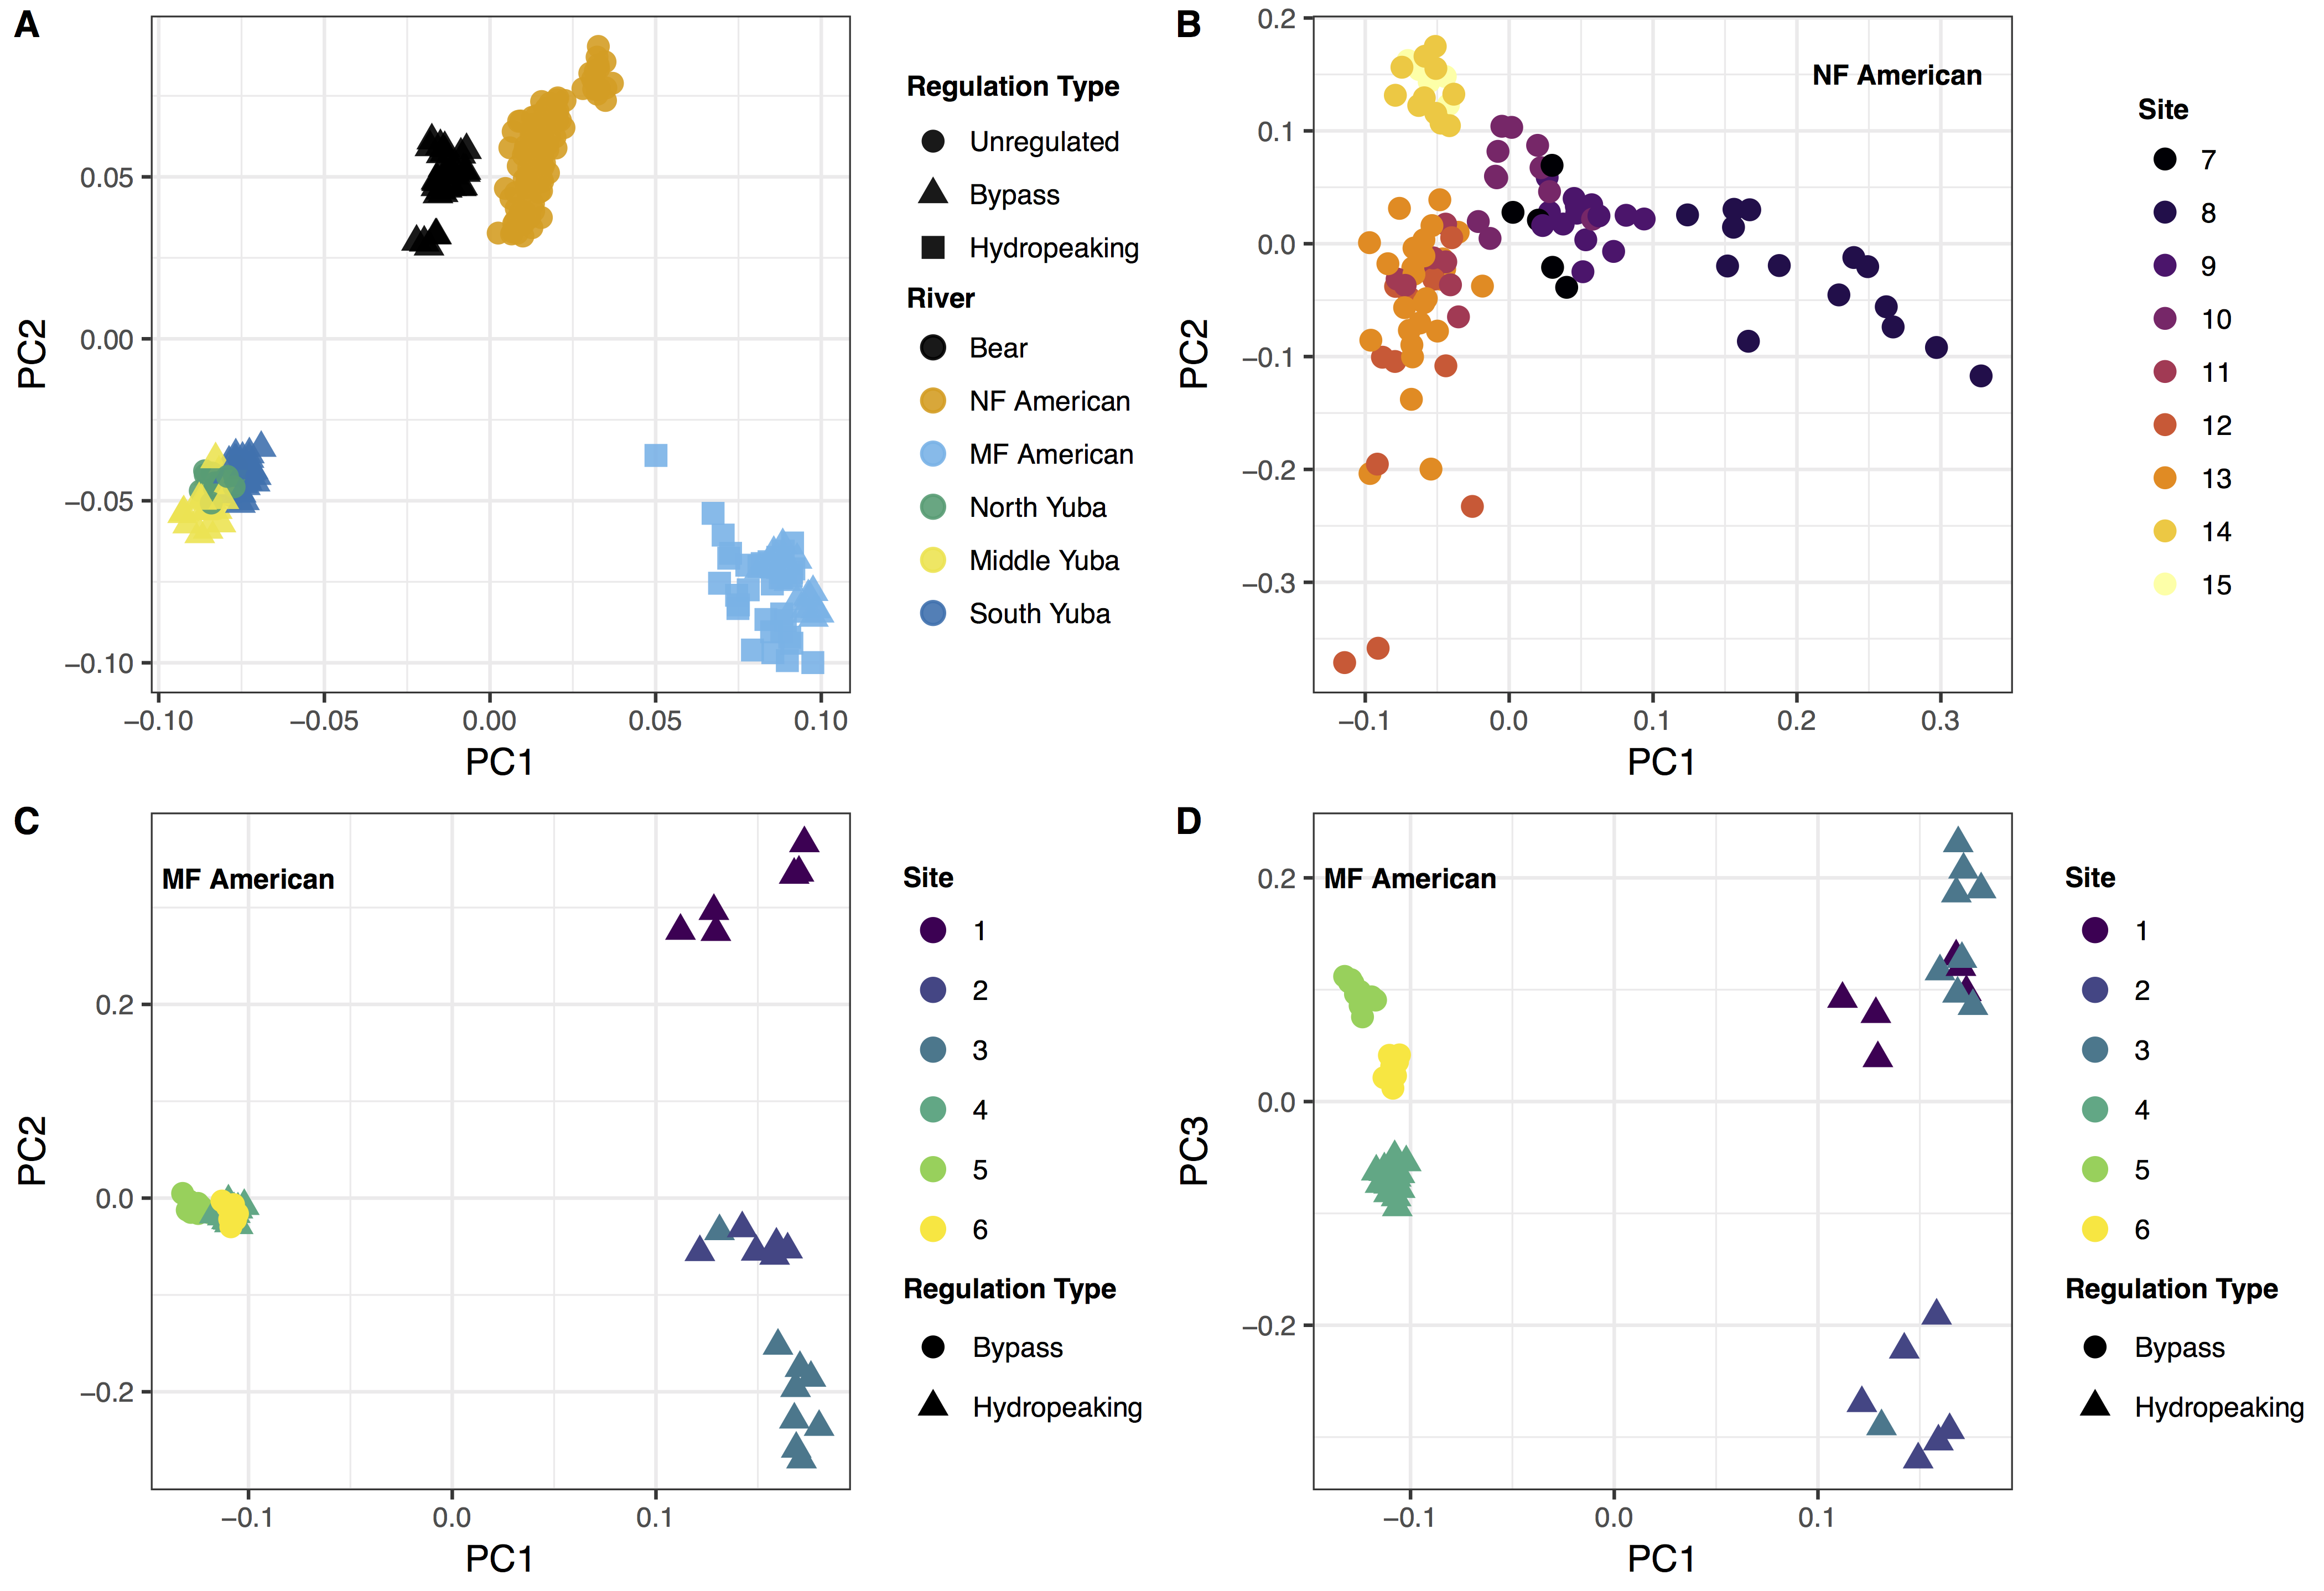
\includegraphics[width=1\linewidth]{figure/ch1/fig_02_pca_combined_v2} \caption{Principal component analysis of Rapture sequencing
data. A) Northern Sierra Nevada (n=277) watersheds and regulation types;
B) Unregulated NF American; C) and D) Hydropeaking MF American Reach.}\label{fig:CH1F2pca}
\end{figure}
To further investigate patterns of genetic variation within the American
watershed, we performed two PCAs, one on samples from the NF American,
and the other on samples from the MF American. The PCA of the NF
American showed minimal differentiation among locations, with different
study sites blending together and weak patterns of population structure
(Figure \ref{fig:CH1F2pca}B). In contrast, PCA of the MF American showed
strong differentiation between sites (Figures \ref{fig:CH1F2pca}C,
\ref{fig:CH1F2pca}D). The MF American PCA completely resolved all sites,
with the first component (PC1) strongly differentiating the samples in
the hydropeaking reach from all other sites in the MF American. This
pattern may be due to the differential river regulation between the two
rivers; the NF American is unregulated and has weak PCA differentiation,
whereas the MF American has a higher level of river regulation and all
sites form distinct genetic clusters, indicative of reduced gene flow
among sites within the MF American.

\hypertarget{river-regulation-is-the-strongest-predictor-of-genetic-isolation-with-r.-boylii-in-the-northern-sierra}{%
\subsection{\texorpdfstring{River regulation is the strongest predictor
of genetic isolation with \emph{R. boylii} in the Northern
Sierra}{River regulation is the strongest predictor of genetic isolation with R. boylii in the Northern Sierra}}\label{river-regulation-is-the-strongest-predictor-of-genetic-isolation-with-r.-boylii-in-the-northern-sierra}}

To assess how patterns of genetic differentiation are associated with
river regulation across our entire study area, we estimated pairwise
F\textsubscript{ST} (Wright
\protect\hyperlink{ref-wright_isolation_1943}{1943}) between all
collection locations within a river for all six rivers. We then plotted
the scaled mean pairwise F\textsubscript{ST} {[}mean F\textsubscript{ST}
/ (1-mean F\textsubscript{ST}){]} (Rousset
\protect\hyperlink{ref-rousset_genetic_1997}{1997}) for each location
against the mean river distance (the average distance along the river
network from each collection location to every other location within
that study river). Furthermore, each location was categorized by
regulation level of closest mainstem location. While there was a clear
relationship between F\textsubscript{ST} and river distance (as shown by
the slope of regression lines in Figure \ref{fig:CH1F3fst}A), there was
a striking pattern of elevated F\textsubscript{ST} by regulation type
(Figure \ref{fig:CH1F3fst}A). Even the bypass regulation type showed a
distinct pattern of elevated F\textsubscript{ST} compared to the
unregulated type. For instance, regulated rivers with locations
separated by less than 10km had F\textsubscript{ST} values comparable to
unregulated locations separated by mean river distances over 30 km.
Hydropeaking was the most extreme pattern of the three regulation types
and showed highly elevated F\textsubscript{ST} values with the steepest
regression coefficient. The baseline F\textsubscript{ST} or global mean
increased by over 0.1 between the unregulated (mean
F\textsubscript{ST}=0.141), and regulated locations (global mean for
bypass F\textsubscript{ST}=0.256, hydropeaking
F\textsubscript{ST}=0.278). This suggests a greater degree of isolation
within sites in regulated river reaches compared with \emph{R. boylii}
populations in unregulated reaches, as larger F\textsubscript{ST} values
represent reductions in heterozygosity due to population subdivision
(Slatkin \protect\hyperlink{ref-slatkin_gene_1987}{1987}). We conclude
\emph{R. boylii} in regulated rivers show patterns of greater population
isolation and loss of heterozygosity compared to frogs in unregulated
locations.

To investigate the relative influence of river regulation compared to
other covariates such as river distance on genetic differentiation
(i.e.~F\textsubscript{ST}), we used boosted regression tree (BRT)
modeling. Covariates included flow regime alteration type, river
distance, watershed variables derived from National hydrology data
(NHD), topographic data, and allele frequency spectrum skew. We found
flow regulation explained the greatest amount of variance in
F\textsubscript{ST} (Figure \ref{fig:CH1F3fst}B). Thus, river regulation
has a larger relative influence than mean river distance between
sampling locations, which is often the most important factor influencing
genetic differentiation (Wright
\protect\hyperlink{ref-wright_isolation_1943}{1943}, Slatkin
\protect\hyperlink{ref-slatkin_gene_1987}{1987}, Rousset
\protect\hyperlink{ref-rousset_genetic_1997}{1997}). We conclude there
is a pattern of isolation and limited connectivity between populations
in regulated reaches.






\begin{figure}
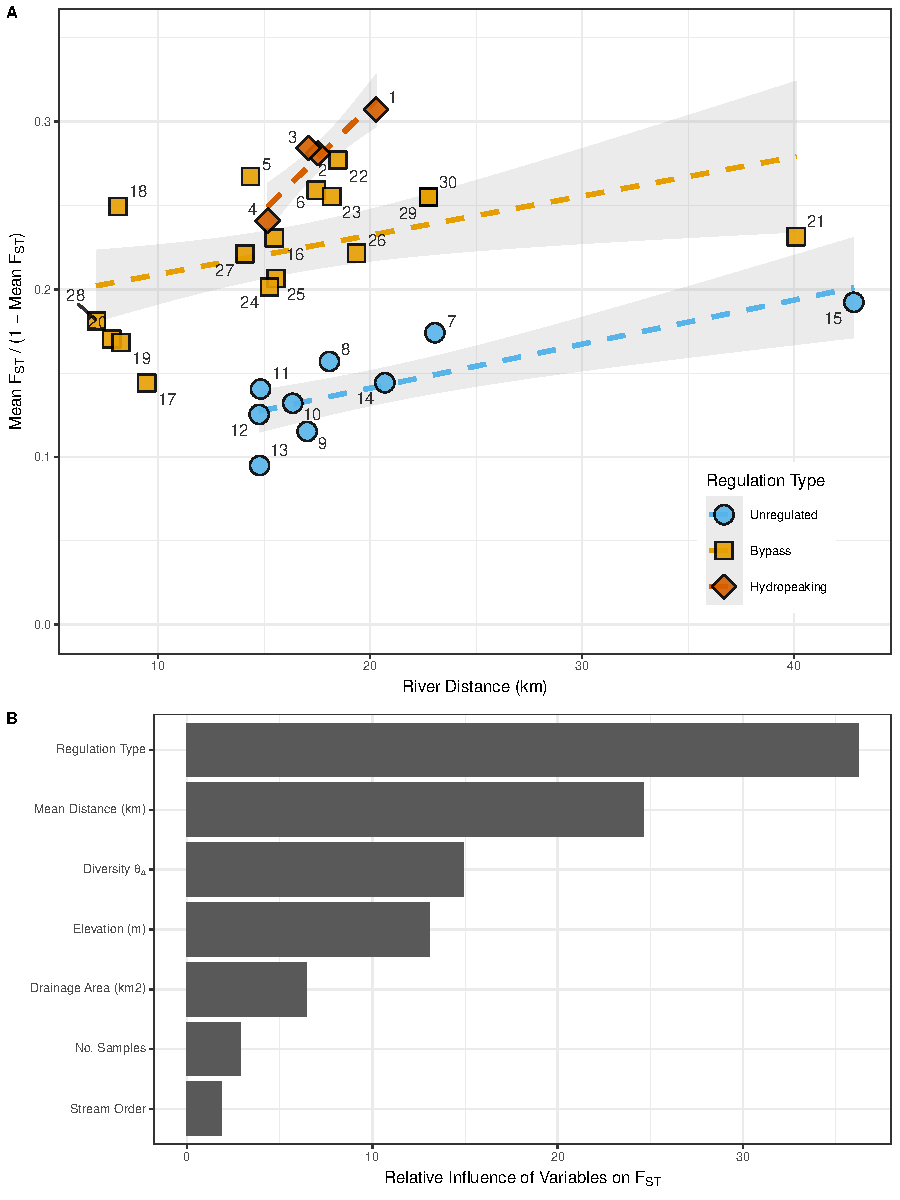
\includegraphics[width=0.9\linewidth]{figure/ch1/fig_03ab_fst_brt_cowplot_for_phd} \caption{Relationship between river regulation and genetic
differentiation in \emph{R. boylii}. A) Mean pairwise
F\textsubscript{ST} vs.~mean river distance for each location; B)
Relative influence of variables on F\textsubscript{ST} from boosted
regression tree models.}\label{fig:CH1F3fst}
\end{figure}
\clearpage

\hypertarget{river-regulation-strongly-correlated-with-decreasing-genetic-diversity-in-r.-boylii}{%
\subsection{\texorpdfstring{River regulation strongly correlated with
decreasing genetic diversity in \emph{R.
boylii}}{River regulation strongly correlated with decreasing genetic diversity in R. boylii}}\label{river-regulation-strongly-correlated-with-decreasing-genetic-diversity-in-r.-boylii}}

To investigate the association between river regulation and genetic
diversity trajectory (stable, increasing, or decreasing), we summarized
patterns of genetic variation using two estimators of \(\theta\)
(\(4N\mu\)): Tajima's \(\theta\) (\(\theta_\pi\)) is based on the
average number of pairwise differences (Tajima
\protect\hyperlink{ref-tajima_evolutionary_1983}{1983}) and Watterson's
\(\theta\) (\(\theta_S\)) is based on the number of segregating sites
(Watterson \protect\hyperlink{ref-watterson_number_1975}{1975}). These
estimators are influenced by the demographic history of a population and
provide information on the trajectory of changes in genetic diversity.
When genetic diversity has been stable, these estimates are generally
equal; but when genetic diversity has been increasing,
\(\theta_\pi > \theta_S\); and when genetic diversity has been
decreasing, \(\theta_S > \theta_\pi\). We found zero populations sampled
within regulated watersheds had evidence of increasing genetic diversity
(e.g., a \(\theta_\pi - \theta_S\) that was less than zero) (Figure
\ref{fig:CH1F4theta}A). The regulated locations showed a clear
trajectory of genetic diversity loss (Figure \ref{fig:CH1F4theta}A,
\ref{fig:CH1F4theta}B). Three of the four hydropeaking locations had the
highest values of \(\Delta\theta\) (\(\theta_\pi - \theta_S\)), and the
global mean was significantly different from other regulation types.
Although some tributary populations within unregulated watersheds also
showed signs of genetic diversity loss, the mean genetic diversity
trajectory at unregulated locations was largely neutral (Figure
\ref{fig:CH1F4theta}B). This indicates populations in the northern
Sierra Nevada which are already limited in number are losing genetic
variation, and river regulation appears to be exacerbating these
patterns. We conclude there is evidence of recent genetic diversity loss
across populations in the regulated river systems, regardless of
regulation type.










\begin{figure}
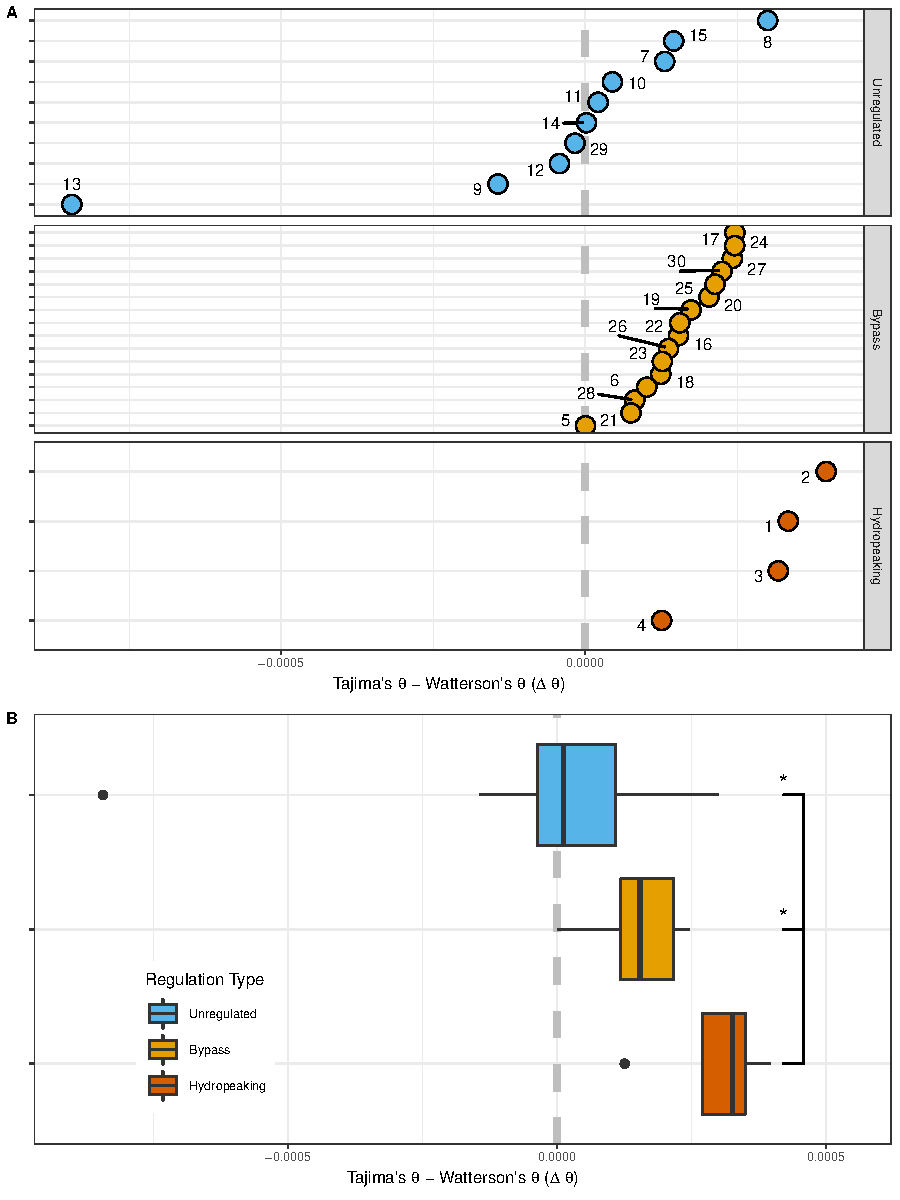
\includegraphics[height=0.8\textheight,scale=1.1]{figure/ch1/fig_04ab_theta_combined_for_phd} \caption{Relationship between river regulation and genetic
diversity trajectory in \emph{R. boylii}. A) Assessment of genetic
diversity trajectories using \(\Delta\theta\)
(\(\theta_\pi - \theta_S\)) for each sampling location; B) Boxplots of
difference between \(\theta_\pi - \theta_S\) and pairwise significance
between regulation groups using a pairwise Wilcoxon rank sum test with
bonferroni correction (P \textless{} 0.05). Negative values represent
trends of increasing genetic diversity, positive values represent
trajectories of diversity loss, values near zero are stable.}\label{fig:CH1F4theta}
\end{figure}
\clearpage

\hypertarget{discussion}{%
\section{Discussion}\label{discussion}}

Although massive parallel sequencing (MPS) technologies have the
potential to facilitate collection of high-quality genetic data in
virtually any species, a number of challenges still remain for many
species including low quality or non-existent reference genomes,
large/complex/repetitive genomes, and high cost of processing/sequencing
in studies with many samples. Amphibians are particularly challenging as
many species have very large genome sizes (Nunziata et al.
\protect\hyperlink{ref-nunziata_genomic_2017}{2017}), for example, there
are only two frog reference genome assemblies available as of 2018
(Hellsten et al. \protect\hyperlink{ref-hellsten_genome_2010}{2010}, Sun
et al. \protect\hyperlink{ref-sun_whole-genome_2015}{2015}). Our results
demonstrate that Rapture (Ali et al.
\protect\hyperlink{ref-ali_rad_2016}{2016}) is a suitable method to
rapidly and inexpensively discover a large number of loci in a frog
species with a complex genome. In this study, we used new RAD sequencing
and RAD capture (Rapture) methods (Ali et al.
\protect\hyperlink{ref-ali_rad_2016}{2016}) to generate high-quality
genomic data suitable for discovering and genotyping many single
nucleotide polymorphisms (SNPs) in \emph{R. boylii}. Based on this
dataset, we were able to successfully characterize patterns of genetic
variation within \emph{R. boylii} as well as design a set of RAD capture
baits that can be used as a genetic monitoring resource for \emph{R.
boylii} (and likely other ranid species). This highlights that the
collection of genetic information, even from large numbers of samples or
in complex genomes, is no longer a limitation with current genomic
methods such as RAD and Rapture.

Demographic connectivity is widely recognized as a fundamental driver of
long-term population persistence (Fahrig and Merriam
\protect\hyperlink{ref-fahrig_habitat_1985}{1985}, Taylor et al.
\protect\hyperlink{ref-taylor_connectivity_1993}{1993}). Populations
must adapt over time and connectivity is a major way to transfer genetic
information. For example, previous studies have shown that adaptation
can occur by spreading specific alleles across large geographic
distances (Miller et al.
\protect\hyperlink{ref-miller_conserved_2012}{2012}, Prince et al.
\protect\hyperlink{ref-prince_evolutionary_2017}{2017}). In many
regulated river reaches in the Sierra Nevada, \emph{R. boylii} now occur
in isolated locations, breeding in tributaries rather than mainstem
habitats. However, since these frogs have the potential to move long
distances (Bourque (\protect\hyperlink{ref-bourque_spatial_2008}{2008})
documented \emph{R. boylii} individuals that moved over 1 km in a day),
the extent to which current population connectivity has been lost due to
river regulation remains unknown. Examining pairwise
F\textsubscript{ST}, revealed a major decrease in connectivity in
populations in regulated systems, even with limited river regulation
(i.e., bypass reaches). Usually isolation by distance patterns best
describe variation in genetic data, yet the primary factor influencing
genetic differentiation among these rivers is hydrologic alteration
(Figure \ref{fig:CH1F3fst}B). Thus, despite being able to move long
distances, \emph{R. boylii} have not been able to maintain population
connectivity in regulated rivers. This demonstrates that even in species
that can move relatively long distances and pass potential physical
barriers (e.g., infrastructure such as dams, canals, and reservoirs
likely do not represent true barriers to movement of \emph{R. boylii}),
loss of connectivity may still occur and can be revealed with genetic
analysis.

Genetic diversity is also a critical component for long-term population
persistence because it is closely related to the evolutionary capacity
for adaptation to environmental changes (Lande and Shannon
\protect\hyperlink{ref-lande_role_1996}{1996}, Frankham
\protect\hyperlink{ref-frankham_introduction_2002}{2002}, Hoffmann and
Sgrò \protect\hyperlink{ref-hoffmann_climate_2011}{2011}, Ishiyama et
al. \protect\hyperlink{ref-ishiyama_differential_2015}{2015}). In some
cases, isolated populations can maintain genetic diversity when they are
sufficiently sized (Whiteley et al.
\protect\hyperlink{ref-whiteley_genetic_2010}{2010}), however, species
of conservation concern typically have small and/or declining
populations and thus may be susceptible to genetic diversity loss (Krohn
et al. \protect\hyperlink{ref-krohn_conservation_2018}{2018}).
Throughout the Sierra Nevada, \emph{R. boylii} have largely disappeared
from regulated mainstem rivers, but the extent to which existing
populations have been able to maintain genetic diversity is unclear.
Strikingly, our analysis revealed that every single population within
the regulated watersheds exhibits a trajectory of genetic diversity
loss. Thus, genomic analysis of molecular variation provides a powerful
lens to discover and assess trajectories of genetic diversity.

Our analyses, using metrics that can serve as a reasonable proxy for
genetic health of a population, does not bode well for the long-term
persistence of \emph{R. boylii} populations in regulated rivers in the
Sierra Nevada. Many of these \emph{R. boylii} populations are already
losing genetic diversity and given their small size and reduced
connectivity the effects of inbreeding will likely exacerbate their
problems. \emph{Rana boylii} have evolved in river systems with
consistent hydrologic seasonality and predictability, despite
inter-annual variation. Flow regulation has altered patterns of
hydrologic seasonality and predictability in many watersheds (Kupferberg
et al. \protect\hyperlink{ref-kupferberg_effects_2012}{2012}). Long-term
population persistence may still be possible if conservation efforts
utilize methods that promote or maintain genetic diversity and increase
population connectivity. For example, simulations by Botero et al.
(\protect\hyperlink{ref-botero_evolutionary_2015}{2015}) demonstrated
adaptation persisted in modeled populations through large environmental
changes---if phenotypic strategies were appropriate before and after the
change---but modeled populations declined rapidly when the current
strategy was a mismatch to the current environment. Thus, \emph{R.
boylii} conservation efforts should focus on river reaches where flow
management may provide opportunities to more closely mimic local natural
flow regimes and improve hydrologic connectivity to prevent further
genetic diversity loss.

\hypertarget{conclusion}{%
\section{Conclusion}\label{conclusion}}

Detecting evolutionary responses to within- and among-year changes in an
ecological or hydrological context has previously been difficult.
However, utilizing genetic data can fill these gaps and provide a highly
informative process for identifying the impacts of anthropogenic and
environmental change on the process of adaptation (Kahilainen et al.
\protect\hyperlink{ref-kahilainen_conservation_2014}{2014}, Botero et
al. \protect\hyperlink{ref-botero_evolutionary_2015}{2015}). We
demonstrate that an aquatic species that has adapted to local hydrology
patterns shows poor genetic health (i.e., clear patterns of decreased
connectivity and trajectories of genetic diversity loss). Our results
highlight the potential impact of river regulation on aquatic organisms
and their potential for long term persistence. In the future, similar
genetic approaches could be used in many other contexts to explore the
impacts of river regulation on aquatic organisms. Taken together, our
results demonstrate that genetic monitoring can be a powerful tool for
assessment of population health and should be a critical component of
conservation management in aquatic organisms.

\hypertarget{hybrids}{%
\chapter{Hybridization between two sympatric ranid frog species in the
northern Sierra Nevada, California}\label{hybrids}}

\hypertarget{introduction-1}{%
\section{Introduction}\label{introduction-1}}

Landscape changes can influence species demography and migration
patterns (Li et al. \protect\hyperlink{ref-li_ten_2017}{2017}) which can
change rates of gene flow within species. Changing migration rates and
population sizes can influence population structure; thus, over time,
landscape changes can cause significant changes in genetic diversity
within a species. Furthermore, cross-breeding or hybridization between
closely related taxa can promote gene flow (introgression) between
species, which may be an important evolutionary mechanism for either
homogenization (reversing initial divergence between species),
speciation (from reproductive isolation of hybrid populations), or
adaptation (transfer of adaptive alleles) (Mallet
\protect\hyperlink{ref-mallet_hybrid_2007}{2007}, Abbott et al.
\protect\hyperlink{ref-abbott_hybridization_2013}{2013}, Barrera-Guzmán
et al. \protect\hyperlink{ref-barrera-guzman_hybrid_2018}{2018}).

Hybridization events in vertebrates may be rare, or rarely detected, and
thus identifying potential hybridization can be difficult and may be
affected by sampling design, timing, and resolution of genetic markers.
Therefore, occurrences of hybridization likely remain unknown,
particularly in cryptic taxa. Assessing population admixture or
detecting potential hybridization has previously been challenging;
however, modern genetic methods provide a powerful approach to assess
populations at fine geographic and evolutionary scales (Ali et al.
\protect\hyperlink{ref-ali_rad_2016}{2016}, Prince et al.
\protect\hyperlink{ref-prince_evolutionary_2017}{2017}).

We investigate the potential for hybridization in two sympatrically
occurring endemic frog species in the Sierra Nevada of California.
Foothill yellow-legged frogs, \emph{Rana boylii}, (Baird
\protect\hyperlink{ref-baird_descriptions_1856}{1856}) historically
occurred in lower and mid-elevation (\textless{}1500 m) streams and
rivers from Southern Oregon to northern Baja California west of the
Sierra-Cascade crest (Stebbins
\protect\hyperlink{ref-stebbins_field_2003}{2003}), whereas Sierra
Nevada yellow-legged frogs, \emph{Rana sierrae}, (Camp
\protect\hyperlink{ref-camp_notes_1917}{1917}) typically occurred from
1500 m to over 3600 m in lakes and streams (Zweifel
\protect\hyperlink{ref-zweifel_ecology_1955}{1955}, Stebbins
\protect\hyperlink{ref-stebbins_field_2003}{2003}). Population declines
have been documented across the former range of both of these species;
\emph{R. sierrae} has been extirpated from over 90 percent of its
historical range (Drost and Fellers
\protect\hyperlink{ref-drost_collapse_1996}{1996}, Vredenburg
\protect\hyperlink{ref-vredenburg_reversing_2004}{2004}) while \emph{R.
boylii} has been extirpated from 50 percent of its historical range
(Jennings and Hayes
\protect\hyperlink{ref-jennings_amphibian_1994}{1994}, Davidson et al.
\protect\hyperlink{ref-davidson_spatial_2002}{2002}). Both species are
of conservation concern; in 2014, the U. S. Fish and Wildlife Service
(USFWS) listed \emph{R. sierrae} as endangered under the U. S.
Endangered Species Act (ESA) (USFWS
\protect\hyperlink{ref-usfws_endangered_2014}{2014}), and \emph{R.
boylii} is listed as a species of special concern in California and is a
candidate for listing under the California and federal ESAs.

Unlike other ranid frog species with broad areas of potential
intergradation (Shaffer et al.
\protect\hyperlink{ref-shaffer_species_2004}{2004}), \emph{R. boylii}
and \emph{R. sierrae} only rarely occur sympatrically. Zweifel
(\protect\hyperlink{ref-zweifel_ecology_1955}{1955}) described one
historical location where these two species co-occurred, in Butte County
near DeSabla. Currently the only known location where both species are
found is several tributaries to the Feather River in the northern Sierra
Nevada, California (Figure \ref{fig:CH2F1map}). Hybridization between
these species has not previously been documented. Furthermore, breeding
experiments by Zweifel
(\protect\hyperlink{ref-zweifel_ecology_1955}{1955}) between \emph{R.
sierrae} (formerly known as \emph{R. muscosa}) and \emph{R. boylii}
yielded very low viability in fertilization and high incidences of
embryological abnormalities---indicating a post-zygotic barrier between
the species. However, these experiments only crossed female \emph{R.
sierrae} with male \emph{R. boylii}, and the individuals were from very
different California regions (e.g., Butte and Nevada County vs.~Contra
Costa County). \emph{Rana boylii} and \emph{R. sierrae} have very
similar morphology and habitat preferences in areas where they co-occur;
thus assigning individuals to species is difficult and imprecise using
field identification methods. This presents a challenge for management
because these sympatric species have different conservation status and
management objectives. We employed modern genetic methodology to better
understand \emph{R. sierrae} and \emph{R. boylii} where their ranges
overlap. We investigated three primary questions:
\begin{enumerate}
\def\labelenumi{\arabic{enumi}.}
\tightlist
\item
  Can hybridization be detected between two sympatrically occurring
  threatened and endangered (ESA) frog species in the Sierra Nevada
  using data generated from genome-wide single nucleotide polymorphisms
  (SNPs);
\item
  If hybrids can be detected, do genetic signatures suggest hybrid
  viability (i.e., can hybrids reproduce, leading to introgression
  between species);
\item
  Using coalescent modeling, are migration rates between species in
  sympatrically occurring populations higher than in allopatrically
  occurring populations in adjacent watersheds?
\end{enumerate}
\hypertarget{methods-1}{%
\section{Methods}\label{methods-1}}

\hypertarget{ch2samplecollection}{%
\subsection{Sampling and DNA Extraction}\label{ch2samplecollection}}

To investigate potential hybridization between \emph{R. sierrae} and
\emph{R. boylii}, a total of 458 tadpole tail clips, buccal swabs, or
tissue samples were compiled. Samples were identified to species in the
field as either \emph{R. boylii}, \emph{R. sierrae}, or ``unknown'',
which were individuals which could not be visually confirmed as either
species (Stebbins \protect\hyperlink{ref-stebbins_field_2003}{2003}).
The samples were collected between 1992 and 2016, from three watersheds
in the Sierra Nevada (the Feather, Yuba, and American) (Table
\ref{tab:CH2T1}, \protect\hyperlink{supptables}{Appendix, S5}). All
unknown individuals were from Feather watershed localities.

The Yuba and American watersheds share a similar Mediterranean climate,
underlying geology, watershed aspect (west-slope), and vegetative
communities. The Feather watershed shares a similar climate but has a
slightly different underlying geology and aspect than that of other
watersheds in the Sierra Nevada. The Feather watershed lies in the
transition zone of the northern Sierra Nevada and the Cascades/Basin and
Range Province, and thus the landscape in the northern portion of the
watershed is comprised largely of volcanic bedrock while the southern
portion is largely granitic (Durrell
\protect\hyperlink{ref-durrell_geologic_1988}{1988}).

\clearpage

\begingroup\fontsize{9}{11}\selectfont
\begin{longtable}[t]{llrllll}
\caption{\label{tab:CH2T1}Sampling localities.}\\
\toprule
Locality & River & No. Samples & Lat. & Lon. & Elev (m) & Basin (HUC8)\\
\midrule
\endfirsthead
\caption[]{\label{tab:CH2T1}Sampling localities. \textit{(continued)}}\\
\toprule
Locality & River & No. Samples & Lat. & Lon. & Elev (m) & Basin (HUC8)\\
\midrule
\endhead
\
\endfoot
\bottomrule
\endlastfoot
MFA-AMEC & MFA & 5 & 38.934 & -120.9436 & 240 & American\\
MFA-GASC & MFA & 1 & 38.9665 & -120.9325 & 242 & American\\
MFA-TODC & MFA & 6 & 38.9638 & -120.9216 & 368 & American\\
MFA-US-R & MFA & 1 & 39.0075 & -120.7316 & 360 & American\\
NFA & NFA & 12 & 39.1079 & -120.9227 & 363 & American\\
\addlinespace
NFA-BUNC & NFA & 8 & 39.0376 & -120.9103 & 286 & American\\
NFA-EUCHDS & NFA & 3 & 39.1849 & -120.762 & 580 & American\\
NFA-INDC & NFA & 3 & 39.0567 & -120.9085 & 296 & American\\
NFA-LyonsPk & NFA & 11 & 39.2067 & -120.3113 & 2529 & American\\
NFA-POND & NFA & 2 & 38.9999 & -120.9406 & 241 & American\\
\addlinespace
NFA-ROBR & NFA & 6 & 39.1045 & -120.9267 & 400 & American\\
NFA-SHIC & NFA & 8 & 39.0417 & -120.9009 & 341 & American\\
NFA-SLAR & NFA & 5 & 39.0987 & -120.9255 & 356 & American\\
NFMFA-SC & NFMFA & 7 & 39.0224 & -120.7369 & 522 & American\\
RUB-HighlandDS & RUB & 18 & 38.9615 & -120.2422 & 2312 & American\\
\addlinespace
RUB-HighlandLk & RUB & 29 & 38.9573 & -120.2418 & 2383 & American\\
RUB-LC-US & RUB & 1 & 38.9889 & -120.69 & 415 & American\\
RUB-USPH & RUB & 5 & 38.9993 & -120.7233 & 361 & American\\
RUB-Zitella & RUB & 9 & 38.9595 & -120.227 & 2335 & American\\
RUB-ZitellaLk & RUB & 2 & 38.9604 & -120.2316 & 2337 & American\\
\addlinespace
SFA-CAMI & SFA & 2 & 38.8115 & -120.5787 & 725 & American\\
FEA-BeanCk & FEA & 60 & 39.9774 & -121.091 & 1397 & Feather\\
FEA-EBNFF & FEA & 6 & Unknown & Unknown & Unknown & Feather\\
FEA-GoldLk & FEA & 4 & 39.9416 & -121.136 & 1816 & Feather\\
FEA-LoneRockCk & FEA & 3 & 40.2012 & -120.6453 & 1563 & Feather\\
\addlinespace
FEA-MillCk & FEA & 4 & 39.9591 & -121.1573 & 1891 & Feather\\
FEA-RockLkBucksCk & FEA & 1 & 39.9403 & -121.1499 & 2102 & Feather\\
FEA-RockLkSilver & FEA & 8 & 39.9409 & -121.1422 & 1902 & Feather\\
FEA-SFRockCk & FEA & 27 & 39.8789 & -121.0022 & 1470 & Feather\\
FEA-SPANISH-BGulch & FEA & 5 & 39.9546 & -121.089 & 1283 & Feather\\
\addlinespace
FEA-SPANISH-RockCk & FEA & 1 & 39.9445 & -121.0221 & 1090 & Feather\\
FEA-SPANISH-SilverCk & FEA & 3 & 39.9377 & -121.0849 & 1189 & Feather\\
FEA-SPANISH-Wapaunsie & FEA & 1 & 39.9523 & -121.0373 & 1096 & Feather\\
FEA-SpanishCk & FEA & 26 & 39.9541 & -121.0541 & 1192 & Feather\\
NFF-Poe & NFF & 1 & 39.736 & -121.4702 & 284 & Feather\\
\addlinespace
FORD-Mossy-P1 & FORD & 1 & 39.381 & -120.4623 & 2157 & Yuba\\
FORD-Mossy-P2 & FORD & 3 & 39.3852 & -120.4714 & 1998 & Yuba\\
FORD-Mossy-P3 & FORD & 2 & 39.3765 & -120.4603 & 2158 & Yuba\\
FORD-MossyDS & FORD & 19 & 39.3853 & -120.4728 & 1984 & Yuba\\
FORD-MossyPond & FORD & 34 & 39.3781 & -120.4701 & 2106 & Yuba\\
\addlinespace
FORD-NorthCkTrib & FORD & 34 & 39.3869 & -120.451 & 2090 & Yuba\\
MFY-OREGCk & MFY & 10 & 39.4419 & -121.0575 & 620 & Yuba\\
MFY-Remmington & MFY & 1 & 39.4137 & -120.9912 & 620 & Yuba\\
MFY-US-OH & MFY & 7 & 39.413 & -120.9903 & 624 & Yuba\\
NFY & NFY & 12 & 39.5119 & -120.9774 & 705 & Yuba\\
\addlinespace
NFY-SLATE-CGRav & NFY & 3 & 39.6928 & -120.9258 & 1457 & Yuba\\
NFY-SLATE-Onion & NFY & 3 & 39.6355 & -121.0395 & 1300 & Yuba\\
SFY & SFY & 1 & 39.3539 & -120.7342 & 890 & Yuba\\
SFY-FallCk & SFY & 5 & 39.3553 & -120.7371 & 884 & Yuba\\
SFY-HUMBUG & SFY & 1 & 39.3637 & -120.921 & 877 & Yuba\\
\addlinespace
SFY-LOGA & SFY & 3 & 39.3691 & -120.8526 & 1201 & Yuba\\
SFY-MCKI & SFY & 3 & 39.368 & -120.8354 & 1084 & Yuba\\
SFY-MISC & SFY & 7 & 39.361 & -120.8814 & 1095 & Yuba\\
SFY-RockCk & SFY & 3 & 39.3298 & -120.9863 & 594 & Yuba\\
SFY-Scotchman & SFY & 3 & 39.3293 & -120.777 & 1167 & Yuba\\
SFY-ShadyCk & SFY & 9 & 39.3543 & -121.059 & 675 & Yuba\\*
\end{longtable}\endgroup{}
\clearpage

Field sampling was conducted following methods in Heyer et al.
(\protect\hyperlink{ref-heyer_measuring_1994}{1994}) under CDFW SCP
permit \#0006881 and federal permit TE-40087B-0 with IACUC protocol
\#19327 and \#04718-001. Individual post-metamorphic frogs were
buccal-swabbed following established protocols (Goldberg et al.
\protect\hyperlink{ref-goldberg_frogs_2003}{2003}, Pidancier et al.
\protect\hyperlink{ref-pidancier_buccal_2003}{2003}, Broquet et al.
\protect\hyperlink{ref-broquet_buccal_2007}{2007}). Each
post-metamorphic individual was comprehensively swabbed underneath
tongue and inside of both cheeks for approximately 30 sec to one minute.
Swabs were air dried for approximately five minutes and placed in 1.5 mL
microcentrifuge tubes while in the field or placed in lysis buffer.
Dried samples were stored in the laboratory at -80°C until DNA
extraction. Where possible, tail clips from tadpole larvae were
collected, and tadpoles greater than 15 mm total length were targeted
(Wilbur and Semlitsch
\protect\hyperlink{ref-wilbur_ecological_1990}{1990}, Parris et al.
\protect\hyperlink{ref-parris_assessing_2010}{2010}). One clip was taken
per individual tadpole and dried on Whatman filter paper (grade 1) and
stored at room temperature or in 95\% ethanol. DNA was extracted from
ethanol-stored samples using Qiagen DNeasy kits following manufacturer
protocol and stored at -20°C. DNA was extracted from dried buccal swabs
and tail clips using an Ampure magnetic bead-based protocol (Ali et al.
\protect\hyperlink{ref-ali_rad_2016}{2016}) and stored at -20°C.

\hypertarget{rapture2}{%
\subsection{Rapture Sequencing}\label{rapture2}}

To produce a high-quality genomic resource for frog species with large
genome sizes, we interrogated a significant fraction of the \emph{R.
boylii} genome using RAD sequencing with SbfI (Miller et al.
\protect\hyperlink{ref-miller_rapid_2007}{2007}, Baird et al.
\protect\hyperlink{ref-baird_rapid_2008}{2008}, Ali et al.
\protect\hyperlink{ref-ali_rad_2016}{2016}). Paired-end sequence data
were generated using 24 \emph{R. boylii} individuals collected
previously (Peek \protect\hyperlink{ref-peek_landscape_2010}{2010}) from
coastal and Sierra Nevada populations in California, USA
\protect\hyperlink{supptables}{(Appendix, S2)}. RAD libraries were
constructed following the protocol described in Ali et al.
(\protect\hyperlink{ref-ali_rad_2016}{2016}). De novo locus discovery
and contig extension were carried out as previously described (Miller et
al. \protect\hyperlink{ref-miller_conserved_2012}{2012}) using the
alignment program Novoalign and the genome assembler PRICE (Ruby et al.
\protect\hyperlink{ref-ruby_price_2013}{2013}). This resulted in a set
of 77,544 RAD contigs ranging from 300 to 800 bp which served as a de
novo partial genome reference for all subsequent downstream analyses
\protect\hyperlink{supptables}{(Appendix, S3)}. We next removed loci
with five or more SNPs, and randomly selected 10,000 loci from the
remaining subset. Of these 10,000 loci, 8,533 were successfully designed
into 120 bp RAD capture baits by Arbor Biosciences
\protect\hyperlink{supptables}{(Appendix, S4)}. Sample libraries were
prepared for sequencing following RAD Capture (Rapture) methods outlined
in Ali et al. (\protect\hyperlink{ref-ali_rad_2016}{2016}). These
samples were then used to identify putative high-quality SNPs following
sequencing.

Sampled individuals were aligned against the de novo partial genome
reference using the BWA-MEM algorithm (Li and Durbin
\protect\hyperlink{ref-li_fast_2010}{2010}, Li
\protect\hyperlink{ref-li_aligning_2013}{2013}), and converted to BAM
format and filtered for properly paired alignments using Samtools (Li et
al. \protect\hyperlink{ref-li_sequence_2009}{2009}). Next, alignments
from three different sequencing runs on an Illumina HiSeq were merged
together and duplicates were removed using Samtools (Li et al.
\protect\hyperlink{ref-li_sequence_2009}{2009}). For all downstream
analysis, we selected individuals that had greater than 25,000
alignments (n=311), which provided sufficient data to investigate
population genetic attributes at broad and fine geographic scales
\protect\hyperlink{supptables}{(Appendix, S5)}.

To generate SNP (i.e., segregating site) data, a probabilistic framework
was used for all population genetic analyses as it does not require
calling genotypes and is suitable for low-coverage sequencing data
(Korneliussen et al.
\protect\hyperlink{ref-korneliussen_calculation_2013}{2013}, Fumagalli
et al. \protect\hyperlink{ref-fumagalli_quantifying_2013}{2013}). SNP
discovery, minor allele frequencies (MAF) estimates, and genotype
probabilities were conducted using ANGSD (Korneliussen et al.
\protect\hyperlink{ref-korneliussen_angsd_2014}{2014}). ANGSD analyses
were conducted following methods from Prince et al.
(\protect\hyperlink{ref-prince_evolutionary_2017}{2017}), with a minimum
mapping quality score (\texttt{minMapQ}) of 10, a minimum base quality
score (\texttt{minQ}) of 20, the genotype likelihood model
(\texttt{GL\ 1}), specifying the Rapture bait locations using the
\texttt{sites} flag, and only sites represented in at least 50\% of the
included samples (\texttt{minInd}) were used. Furthermore, genomic sites
were designated as polymorphic only if MAFs were greater than 0.05 and
the probability of the site not being polymorphic was less than
1e\textsuperscript{-6}. Using this approach, over 44,000 polymorphic
sites were identified across all \emph{R. boylii} study samples.

\hypertarget{pca-and-admixture}{%
\subsection{PCA and Admixture}\label{pca-and-admixture}}

To assess population structure and coancestry, ANGSD was used to
generate PCA and NGSadmix was used to calculate admixture. Settings used
in ANGSD for PCA to identify polymorphic sites included a
\texttt{SNP\_pval} of 1e\textsuperscript{-6}, inferring major and minor
alleles (\texttt{doMajorMinor} 1), estimating genotypic likelihoods
(\texttt{GL\ 1}), estimating allele frequencies (\texttt{doMaf\ 2}) (Kim
et al. \protect\hyperlink{ref-kim_estimation_2011}{2011}), retaining
SNPs with a minor allele frequency of at least 0.05 (\texttt{minMaf}),
specifying the Rapture bait locations using the \texttt{sites} flag,
estimation of genotype posterior probabilities using a uniform prior
(\texttt{doPost\ 2}), and the \texttt{doIBS\ 1} and \texttt{doCov\ 1}
options. Principal components (PC) summarizing population structure were
derived from classic eigenvalue decomposition and were visualized using
the ggplot2 package in R (R Core Team
\protect\hyperlink{ref-r_core_team_r_2017}{2017}). To assess admixture
between \emph{R. sierrae} and \emph{R. boylii}, genotype likelihood data
(\texttt{GL\ 1}) was generated in ANGSD with the same settings as above,
in addition to retaining only SNPs that were shared in at least of 50\%
of the samples, \texttt{doPost\ 2}, \texttt{doGLF\ 2}, and limiting to
higher quality alignment data (\texttt{minMapQ\ 10}, \texttt{minQ\ 20}).
We then used NGSadmix (Skotte et al.
\protect\hyperlink{ref-skotte_estimating_2013}{2013}) to infer ancestry
proportions in \emph{R. sierrae} and \emph{R. boylii} individuals.
NGSadmix is a robust admixture method that can be applied to low-depth
NGS data, and does not require called genotypes, thus reducing error
associated with potential ascertainment and uncertainty in the data
(Skotte et al. \protect\hyperlink{ref-skotte_estimating_2013}{2013}).

\hypertarget{f1vsf2}{%
\subsection{F1 vs.~F2 Test with Species Diagnostic SNPs}\label{f1vsf2}}

To test whether hybrids were first generation filial (F1) hybrids or
progeny from F1 hybrids from subsequent generations (e.g., F2, F3,
etc.), we identified differentially fixed (i.e., species-specific) SNPs
and assessed heterozygosity at these loci in hybrid individuals. F1 and
F2 hybrid individuals should exihibit different degrees of
heterozygosity in species-diagnostic SNPs. We called genotypes in ANGSD
using a uniform prior (\texttt{doPost\ 2}) and the following settings:
\texttt{GL\ 1}, \texttt{doGeno\ 13}, \texttt{postCutoff\ 0.95},
\texttt{doMaf\ 1}, \texttt{doMajorMinor\ 1}, \texttt{minInd\ 2},
\texttt{SNP\_pval\ 1e-6}, \texttt{minMapQ\ 20}, \texttt{minQ\ 20}, and
specifying the Rapture bait locations using the \texttt{sites} flag. The
subsequent output (\texttt{*.geno.gz}) was then processed in the program
R using the dplyr package (Wickham et al.
\protect\hyperlink{ref-wickham_dplyr_2018}{2018}) to manipulate and
filter to homozygous diagnostic SNPs. Data were filtered to include only
loci where over 50 non-hybrid individuals from each species had called
genotypes at a given polymorphism.

\hypertarget{demographic-modeling-with-fastsimcoal2}{%
\subsection{Demographic Modeling with
fastsimcoal2}\label{demographic-modeling-with-fastsimcoal2}}

To quantify divergence times and migration rates between \emph{R.
sierrae} and \emph{R. boylii}, we used coalescent simulations in
fastsimcoal2 (Excoffier and Foll
\protect\hyperlink{ref-excoffier_fastsimcoal_2011}{2011}, Excoffier et
al. \protect\hyperlink{ref-excoffier_robust_2013}{2013}). This
maximum-likelihood modeling approach uses simulations to estimate the
expected site-frequency spectra (SFS) for a demographic model of
interest to calculate a composite likelihood, and then utilizes a
maximization procedure to find the maximum-likelihood parameter
estimates.

We calculated folded joint SFS for each species in each watershed from
SNP data generated from ANGSD because the ancestral condition is
unknown. For all models, we assumed the potential for bidirectional gene
flow and that extant genetic clusters emerged simultaneously from a
common ancestry. We tested models that allowed for population growth,
and models with no growth. We used two conservative model scenarios to
estimate divergence times and migration rates between species in each
watershed. To estimate migration probabilities per generation between
species within each watershed, we set the divergence time parameters
between 1--1.1 billion years ago to create simplified migration-only
models. To estimate divergence time between species, we used the
watershed that had the lowest migration rate from the previous
migration-only models, and generated divergence time estimates assuming
no migration between species.

The basic steps taken to obtain final model estimates from fastsimcoal2
used a set of 25 replicate models, followed by comparison of maximum
observed and expected likelihoods to select the best-fit model (Akaike
\protect\hyperlink{ref-akaike_information_1973}{1973}), then simulate
new SFS using the best-fit model for parametric bootstrapping. Following
Excoffier and Foll
(\protect\hyperlink{ref-excoffier_fastsimcoal_2011}{2011}), we used
1,000 randomly drawn SNPs from each SFS to generate 100,000 coalescent
simulations for likelihood calculations (estimation of the expected SFS)
with a maximum of 40 cycles for the conditional maximization algorithm.
To select the best-fit model we selected the model replicate that
minimized the difference between the maximum expected likelihood and the
maximum observed likelihood. We used parametric bootstrapping to
generate 95\% confidence intervals for each best-fit model using 100
bootstraps for each model and selected the best model from each
bootstrap based on maximum likelihoods as described above.

\hypertarget{results-1}{%
\section{Results}\label{results-1}}

\hypertarget{rapture-produced-high-quality-genomic-data-for-both-r.-sierrae-and-r.-boylii}{%
\subsection{\texorpdfstring{Rapture produced high quality genomic data
for both \emph{R. sierrae} and \emph{R.
boylii}}{Rapture produced high quality genomic data for both R. sierrae and R. boylii}}\label{rapture-produced-high-quality-genomic-data-for-both-r.-sierrae-and-r.-boylii}}

Individual samples were collected across 56 different sampling
localities in three different watersheds (Figure \ref{fig:CH2F1map},
Table \ref{tab:CH2T1}). For downstream analysis, we filtered and
retained 311 samples from the original sequencing data that contained a
minimum of 25,000 alignments \protect\hyperlink{supptables}{(Appendix,
S5)}. The final merged dataset mean alignments per sample was 229,485
\protect\hyperlink{supptables}{(Appendix, S5)}, and the mean number of
samples per site was eight. These frog species are cryptic, and often
occur in low densities, so we retained all sites in our analysis,
regardless of the number of samples per locality (Table
\ref{tab:CH2T1}). We conclude that the sequence data we obtained should
be appropriate for population genetic analyses across our study area.



\begin{figure}
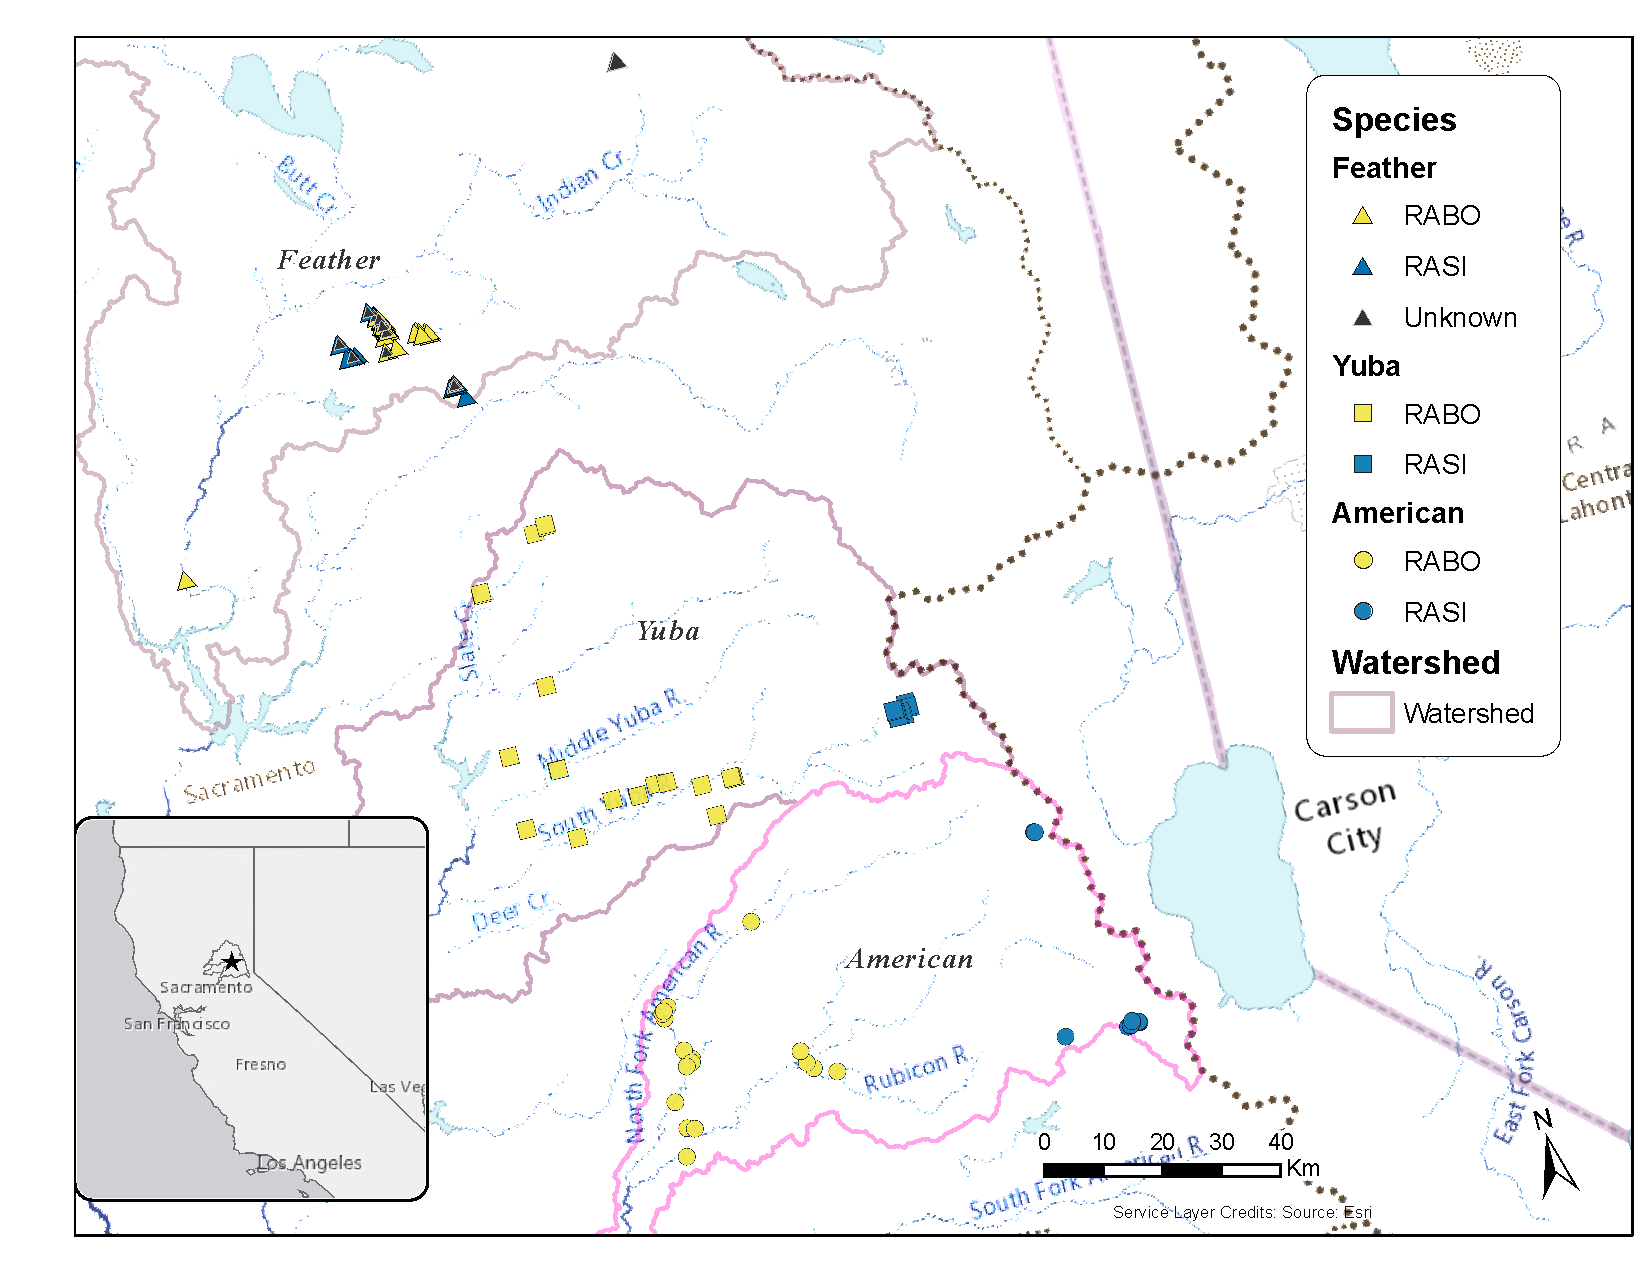
\includegraphics[angle=90, scale=.70]{figure/ch2/figure_01_overview_hybrid} \caption{Map of sampling locations in the Feather, Yuba, and
American watersheds. RABO=\emph{R. boylii}, RASI=\emph{R. sierrae}.}\label{fig:CH2F1map}
\end{figure}
\clearpage

\hypertarget{pca-shows-strong-separation-between-species-and-identifies-putative-hybrids}{%
\subsection{PCA shows strong separation between species and identifies
putative
hybrids}\label{pca-shows-strong-separation-between-species-and-identifies-putative-hybrids}}

To assess within-basin population structure, principal components
analysis (PCA) was used to provide a dimensionless comparison of
putative SNPs across species and watersheds (Figure \ref{fig:CH2F2pca}).
Strong differentiation was observed between species (\emph{R. sierrae}
and \emph{R. boylii}) on the PC1 axis, which accounted for approximately
55 percent of the variation. PC2 differentiated \emph{R. sierrae} among
the three watersheds (Figure \ref{fig:CH2F2pca}A), while PC3
differentiated \emph{R. boylii} sampling locations among the three
watersheds (Figure \ref{fig:CH2F2pca}B). Little sign of admixture
between the two species appears in the PCA, however, two
samples---collected in the Feather watershed and designated as
``unknown'' in the field---clustered halfway between the \emph{R.
sierrae} and \emph{R. boylii} groups along PC1, suggesting these
individuals were hybrids.




\begin{figure}

{\centering 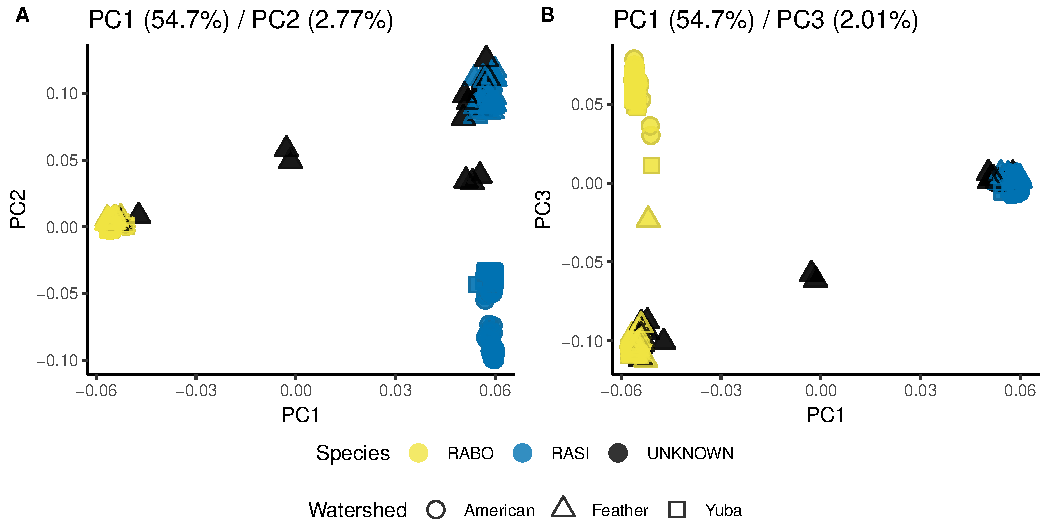
\includegraphics[width=0.95\linewidth]{figure/ch2/figure_02_pca_rasi_all_25k_combined} 

}

\caption{Principal component analysis of Rapture sequencing data,
RABO=\emph{R. boylii}, RASI=\emph{R. sierrae}. A) PC1 vs.~PC2; B) PC1
vs.~PC3.}\label{fig:CH2F2pca}
\end{figure}
\clearpage

\hypertarget{admixture-shows-two-unknown-individuals-with-equal-rana-species-ancestry}{%
\subsection{\texorpdfstring{Admixture shows two unknown individuals with
equal \emph{Rana} species
ancestry}{Admixture shows two unknown individuals with equal Rana species ancestry}}\label{admixture-shows-two-unknown-individuals-with-equal-rana-species-ancestry}}

To further investigate if the two unknown individuals identified in the
PCA were potential hybrids of \emph{R. sierrae} and \emph{R. boylii}, we
used NGSAdmix to assess population structure and individual ancestry
from genome-wide SNPs (Skotte et al.
\protect\hyperlink{ref-skotte_estimating_2013}{2013}). We used k=2 to
evaluate the fraction of ancestry derived from each species. Admixture
showed the same two unknown samples from the Feather basin had
approximately 50\% ancestry from each species (\emph{R. boylii} and
\emph{R. sierrae}), confirming their hybrid ancestry (Figure
\ref{fig:CH2F3admix}). Furthermore, ancestry in the individuals
designated as ``unknown'' in the field also showed very low levels of
mixed ancestry between the species. There were very low or nearly
non-existent levels of mixed-ancestry in the American and Yuba basins as
compared to the Feather. However, introgression between \emph{R.
sierrae} and \emph{R. boylii} appears asymmetric, with a greater
proportion of ancestry from \emph{R. boylii} occurring in the \emph{R.
sierrae} samples, particularly in the Feather watershed, and
predominantly in the ``unknown'' individuals. The putative hybrid
individuals were sampled in Bean Creek, a tributary to Spanish Creek
((Figure \ref{fig:CH2F4hybmap}). Bean Creek was one of the only
tributaries where both \emph{R. sierrae} and \emph{R. boylii} co-occur;
therefore we conclude there is strong evidence for recent hybridization
between \emph{R. sierrae} and \emph{R. boylii} in this drainage.




\begin{figure}

{\centering 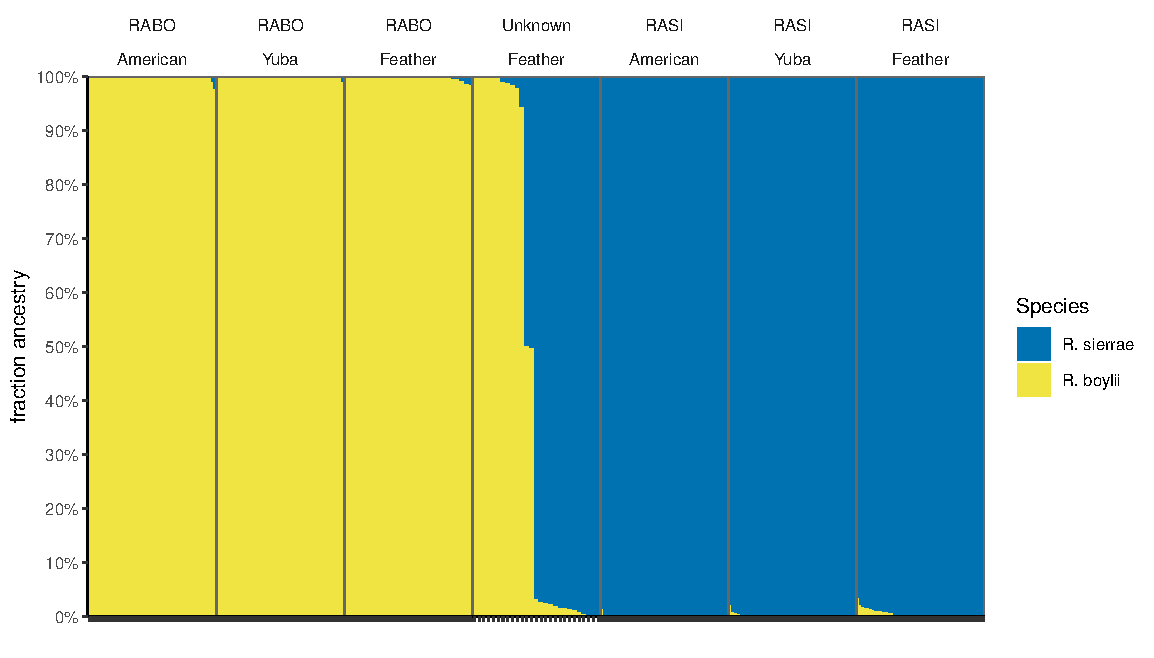
\includegraphics[width=1\linewidth]{figure/ch2/figure_03_admix_rana_by_watershed_25k_k2} 

}

\caption{Admixture (k=2) of \emph{R. sierrae} and \emph{R.
boylii} and ``Unknown'' \emph{Rana} samples from the Feather, American,
and Yuba watersheds.}\label{fig:CH2F3admix}
\end{figure}



\begin{figure}

{\centering 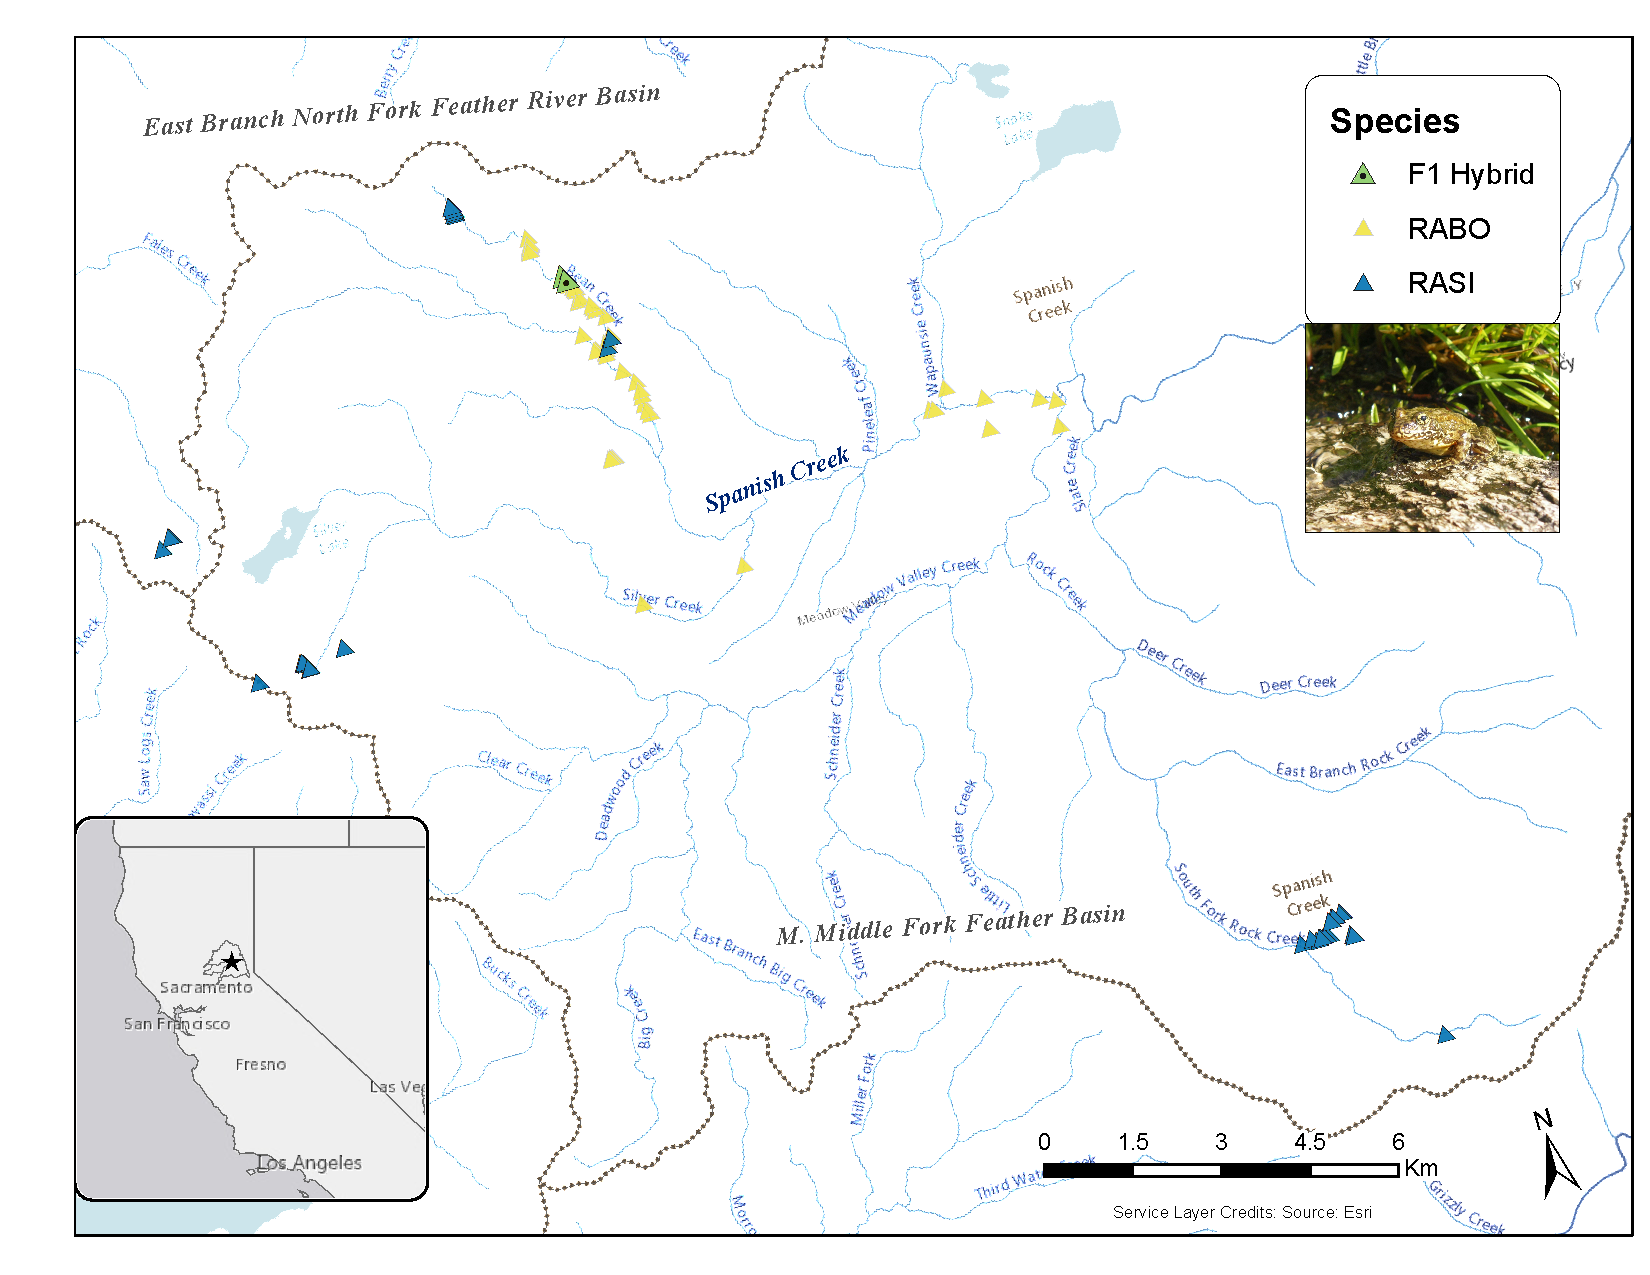
\includegraphics[angle=90, scale=.70]{figure/ch2/figure_04_hybrid_bean_ck} 

}

\caption{Map of sample locations in Bean Creek/Spanish Creek in
the Feather watershed where hybrids were identified. RABO=\emph{R.
boylii}, RASI=\emph{R. sierrae}.}\label{fig:CH2F4hybmap}
\end{figure}
\clearpage

\hypertarget{f1-vs.f2-test-on-hybrids}{%
\subsection{F1 vs.~F2 test on hybrids}\label{f1-vs.f2-test-on-hybrids}}

To test whether the hybrids were F1 (first-generation) or F2 (progeny of
two F1's), we identified species diagnostic SNPs. Our filtering process
(see \protect\hyperlink{f1vsf2}{Methods}) yielded 3,062 putative
diagnostic SNPs that were homozygous for different alleles in \emph{R.
sierrae} or \emph{R. boylii} samples and also had successfully called
genotypes in the two hybrid individuals. F1 hybrids should be
exclusively heterozygous at species diagnostic SNPs. In contrast, F2
hybrids should heterozygous for 50\% of the species diagnostic SNPs, and
homozygous at the remaining 50\% with 25\% allotted to each species. We
observed extremely high heterozygosity and very low homozygosity (6\%
genotyped as \emph{R. boylii}, 4\% \emph{R. sierrae}, and 89\% were
heterozygous) (Figure \ref{fig:CH2F5gentest}). This level of
heterozygosity is far greater than expected for F2 individuals, and the
presence of homozygous genotype calls in the hybrid individuals at
species diagnostic SNPs is expected due to low coverage sequencing data;
genotyping from low coverage sequencing will cause a low frequency of
erroneous homozygous calls, because only one of the two alleles is
sampled, causing heterozygotes to be called as homozygotes. We conclude
these hybrid individuals are F1 instead of F2 individuals. Furthermore,
the hybrid individuals were found to have \emph{R. sierrae}
mitochondrial DNA (Bedwell and Goldberg, in review), indicating the
female was from a \emph{R. sierrae} individual and the male was from
\emph{R. boylii} in both cases.




\begin{figure}

{\centering 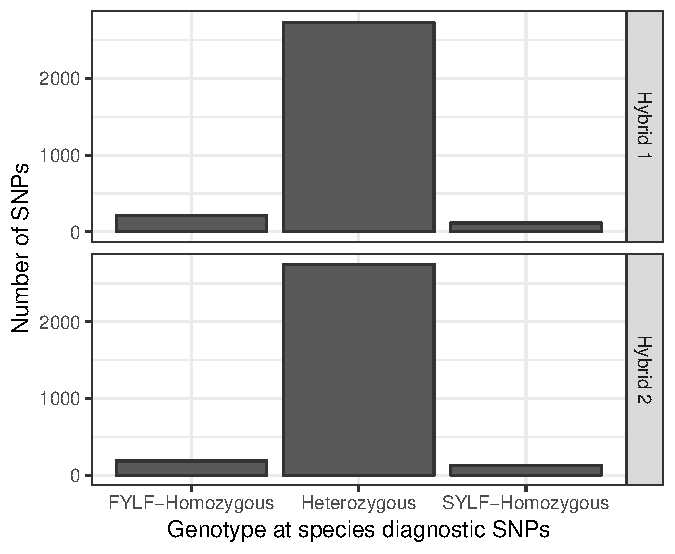
\includegraphics[width=1\linewidth]{figure/ch2/figure_05_f1_f2_hybrid_test_faceted} 

}

\caption{The F1 vs.~F2 test using species diagnostic SNPs to
assess heterozygosity in hybrid individuals. RABO=\emph{R. boylii},
RASI=\emph{R. sierrae}.}\label{fig:CH2F5gentest}
\end{figure}
\clearpage

\hypertarget{divergence-times-and-migration-rates}{%
\subsection{Divergence times and migration
rates}\label{divergence-times-and-migration-rates}}

To test for differential migration rates between \emph{R. sierrae} and
\emph{R. boylii} in the Feather watershed compared to the Yuba and
American, we used fastsimcoal2 (Excoffier and Foll
\protect\hyperlink{ref-excoffier_fastsimcoal_2011}{2011}) coalescent
simulations. Using all individuals except the two hybrid individuals, we
found migration probability (or the per generation likelihood that any
gene from one population transfers to another) from \emph{R. sierrae}
and \emph{R. boylii} was highest in the Feather, with a mean of
5.29e\textsuperscript{-6} (95\% CI
5.28e\textsuperscript{-6}--5.30e\textsuperscript{-6}) and lowest in the
American watershed, 7.80e\textsuperscript{-7}
(7.78e\textsuperscript{-7}--7.81e\textsuperscript{-7})(Figure
\ref{fig:CH2F6fsc}). The migration probabilities in the Yuba watershed
were lower than estimates from the Feather, but were closer in
magnitude, 3.84e\textsuperscript{-6}
(3.83e\textsuperscript{-6}--3.85e\textsuperscript{-6}). We found
migration rates from \emph{R. boylii} to \emph{R. sierrae} were
extremely low across all three (Feather = 6.05e\textsuperscript{-7}
{[}6e\textsuperscript{-7}--6.10e\textsuperscript{-7}{]}, Yuba =
3.76e\textsuperscript{-7}
{[}3.73e\textsuperscript{-7}--3.79e\textsuperscript{-7}{]}, American =
8.29e\textsuperscript{-8}
{[}8.23e\textsuperscript{-8}--8.35e\textsuperscript{-8}{]}; mean and
95\% CI) (Figure \ref{fig:CH2F6fsc}A). As observed in the admixture
analysis, migration rates were asymmetric, showing F1 individuals
backcrossing to individuals from \emph{R. boylii} more often than to
\emph{R. sierrae}. We conclude migration probability rates are highest
in the Feather watershed from \emph{R. sierrae} and \emph{R. boylii},
with very limited migration occurring from \emph{R. boylii} to \emph{R.
sierrae}.





\begin{figure}

{\centering 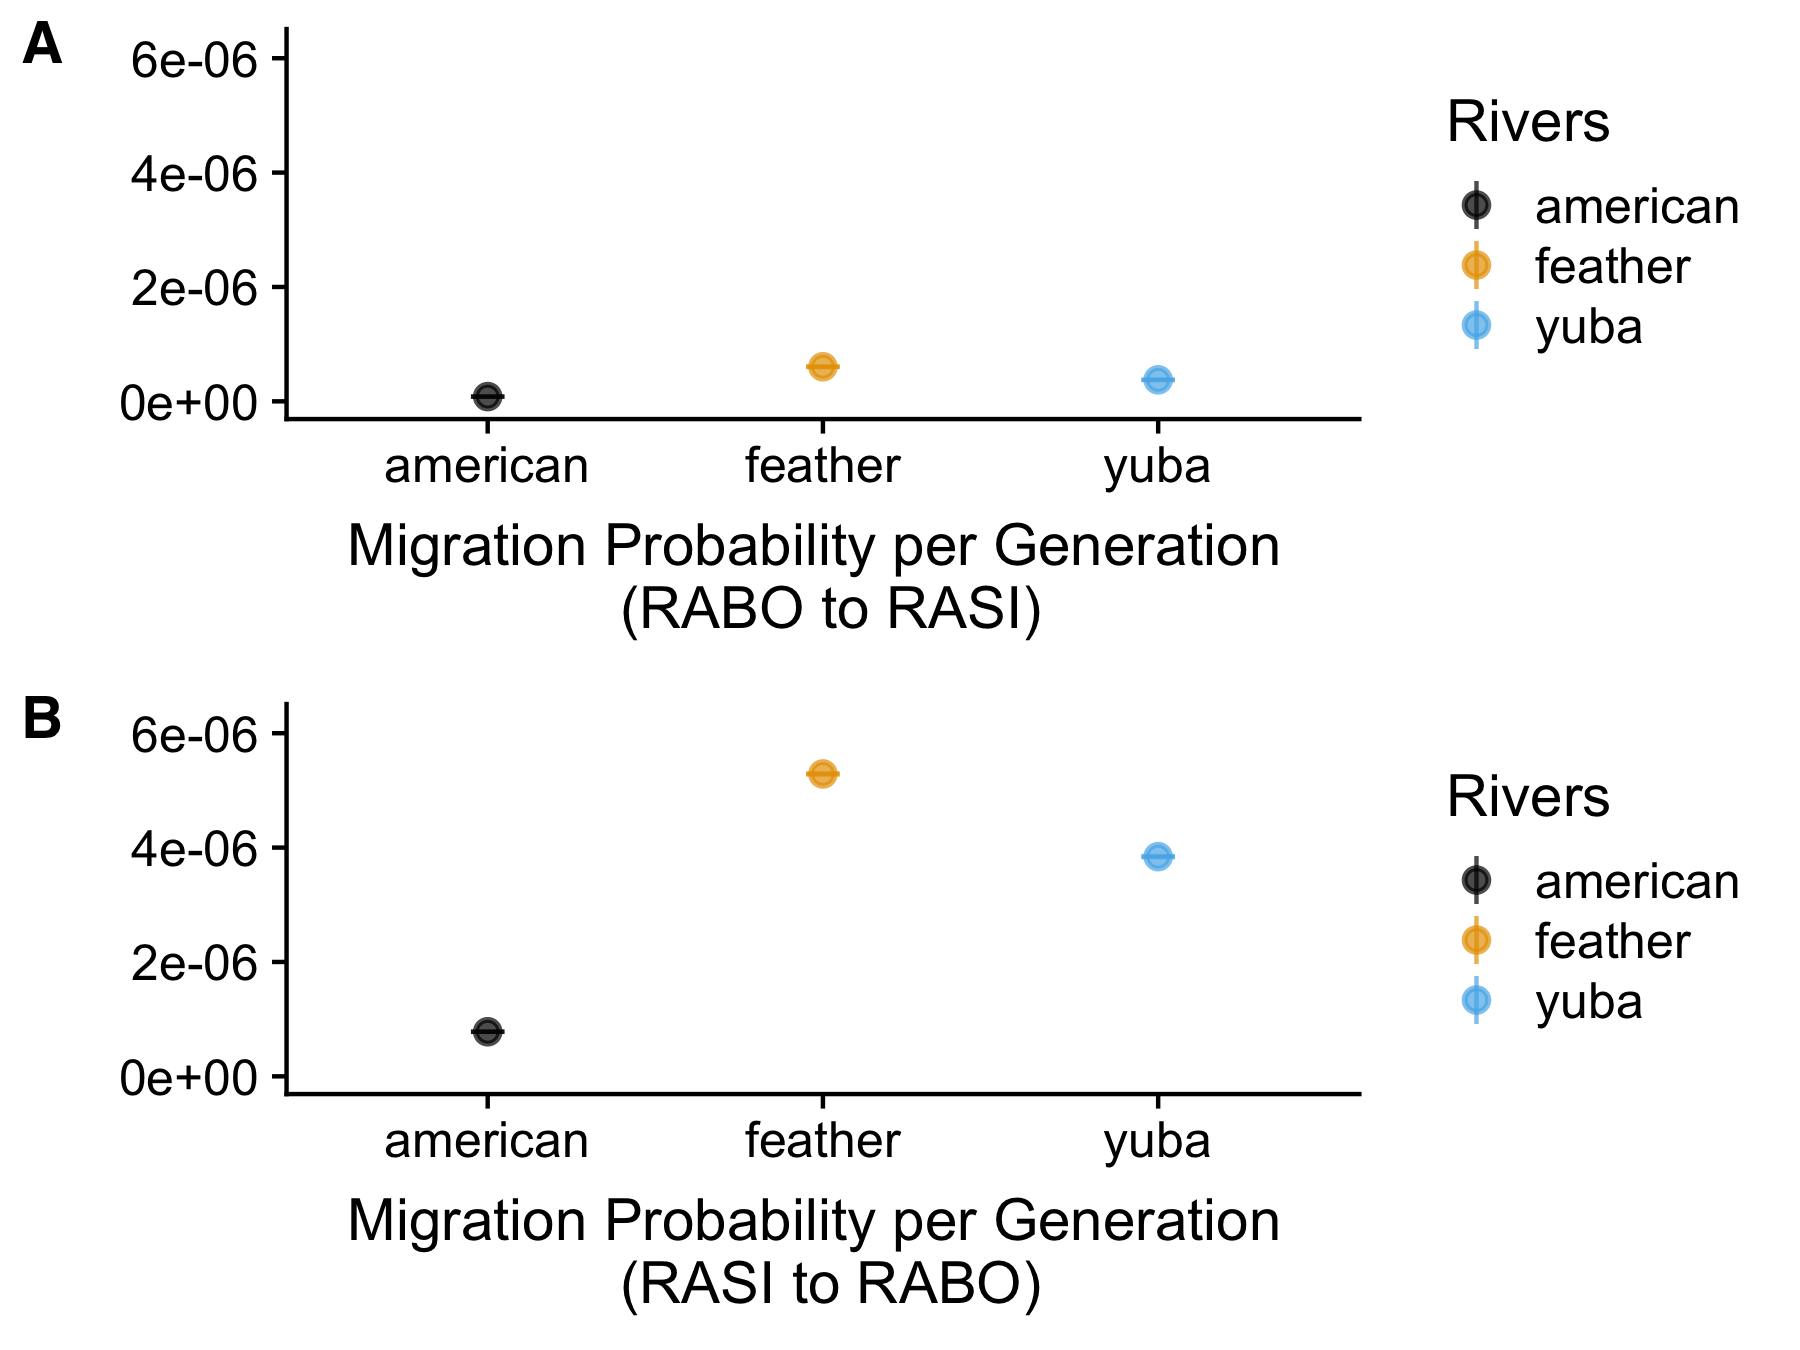
\includegraphics[width=1\linewidth]{figure/ch2/figure_06_coalescent_ancMigration_ptsCI} 

}

\caption{Estimates of migration probabilities from fastsimcoal2
models between the two species within the Feather, Yuba, and American
watersheds. RABO=\emph{R. boylii}, RASI=\emph{R. sierrae}, with 95\%
confidence intervals from 100 bootstrapped estimates.}\label{fig:CH2F6fsc}
\end{figure}
To estimate divergence time between species, we used the American
watershed samples because migration estimates between \emph{R. sierrae}
and \emph{R. boylii} were lowest, and we wanted to derive a conservative
estimate of divergence by minimizing inaccuracy caused by migration. We
ran fastsimcoal2 models with no migration and divergence times bounded
between 10 kya and 4 mya. The best model based on maximum likelihood
estimated the time since divergence between \emph{R. sierrae} and
\emph{R. boylii} was 370,856 (95\% CI: 370,041--371,670) generations.
Typically, \emph{R. boylii} have a generation time of 2--3 years,
depending on the region (Kupferberg et al.
\protect\hyperlink{ref-kupferberg_pulsed_2009}{2009}, Railsback et al.
\protect\hyperlink{ref-railsback_modeling_2015}{2015}), while \emph{R.
sierrae} can have a greater range of generation times, between 3--6
years because tadpoles may overwinter as many as three years (Knapp et
al. \protect\hyperlink{ref-knapp_developing_2003}{2003},
\protect\hyperlink{ref-knapp_large-scale_2016}{2016}). We may assume the
ancestral condition was derived from \emph{R. boylii} (Macey et al.
\protect\hyperlink{ref-macey_molecular_2001}{2001}, Vredenburg et al.
\protect\hyperlink{ref-vredenburg_concordant_2007}{2007}, Yuan et al.
\protect\hyperlink{ref-yuan_spatiotemporal_2016}{2016}), therefore we
suggest a generation time between two and three years, which means
\emph{R. sierrae} likely diverged from \emph{R. boylii} 741 kya to 1.1
mya. This time period corresponds to the early Pleistocene during an era
of episodic glaciation (``the Great Ice Age'')---where distributions
likely contracted and lineages became isolated---followed by subsequent
interglaciation, where distributions expanded (Birkeland
\protect\hyperlink{ref-birkeland_pleistocene_1964}{1964}, Gillespie and
Zehfuss \protect\hyperlink{ref-gillespie_glaciations_2004}{2004}).

\hypertarget{discussion-1}{%
\section{Discussion}\label{discussion-1}}

We identified strong divergence between \emph{R. sierrae} and \emph{R.
boylii} across all three watersheds, evidence of two F1 hybrids, and low
levels of asymmetric introgression primarily in the Feather basin.
Hybridization between \emph{R. sierrae} and \emph{R. boylii} has not
been previously documented based on field observations and breeding
experiments (Zweifel
\protect\hyperlink{ref-zweifel_ecology_1955}{1955}).

It is unlikely that there is currently the potential for major
introgression between \emph{R. sierrae} and \emph{R. boylii},
particularly as hybridization initially may not be adaptive and is often
selected against (Abbott et al.
\protect\hyperlink{ref-abbott_hybridization_2013}{2013}, Streicher et
al. \protect\hyperlink{ref-streicher_diversification_2014}{2014}).
Although hybridization may be common between some amphibian species
(Malone and Fontenot \protect\hyperlink{ref-malone_patterns_2008}{2008})
and can even occur between highly divergent taxa---up to 21 million
years divergent (Prager and Wilson
\protect\hyperlink{ref-prager_slow_1975}{1975})---our data show there is
strong pattern of divergence between \emph{R. sierrae} and \emph{R.
boylii} with limited hybridization and introgression between the
species. Furthermore, there are currently few localities where \emph{R.
sierrae} and \emph{R. boylii} occur sympatrically, and populations of
either species are typically sparse in the Sierra (Kupferberg et al.
\protect\hyperlink{ref-kupferberg_effects_2012}{2012}, Catenazzi and
Kupferberg \protect\hyperlink{ref-catenazzi_importance_2013}{2013}).
Additionally, these two species may be strongly influenced by elevation
due to life history differences (\emph{R. sierrae} are typically found
in higher elevations and are capable of overwintering as tadpoles while
\emph{R. boylii} are not). Previous work suggests that elevation
strongly influences genetic structure in frogs (Monsen and Blouin
\protect\hyperlink{ref-monsen_extreme_2004}{2004})---further reinforced
by the patterns of strong divergence between species within watersheds
that we observe in our data.

There remains the potential for low-levels of naturally occurring
hybridization and introgression between \emph{R. sierrae} and \emph{R.
boylii}, but currently both species appear to have clear genotypic
divergence even in an area of sympatry. Thus, our data suggest this is
unlikely to be a major concern for conservation management. While there
is a potential for misclassification of individuals in intermediate
locations, genetic testing, and/or monitoring could be a useful tool for
clarifying species and population boundaries as well as population size
estimates. Successful tests of not only hybridization, but timing of
divergence events (as well as better understanding bottlenecks and
population expansion) based on landscape history can be informative in
understanding what events may have driven divergence. The landscape of
the Sierra Nevada during the Pleistocene epoch was one of repeated
glaciation (Moore and Moring
\protect\hyperlink{ref-moore_rangewide_2013}{2013}). Rivers flowing into
the present-day Central Valley were being alternately eroded by
west-flowing streams during interglaciation or covered in glaciers. It
is therefore likely that adaptation to colder climates (e.g., freezing
lakes and streams) may have provided an advantage to individuals or
populations occurring in localities where the effects of glaciation were
most prominent. \emph{Rana sierrae} are uniquely adapted to persist in
short-growing periods common in the high Sierras---tadpoles may
overwinter multiple years before metamorphosing---thus \emph{R. sierrae}
may have diverged from \emph{R. boylii} because of their ability to
persist in colder climates, common during periods of glaciation during
the Pleistocene.

While timing of \emph{R. sierrae} and \emph{R. boylii} divergence in the
Sierra Nevada may correspond with the onset of the Pleistocene
glaciation, more recent anthropogenic changes may be a stronger driver
of current population connectivity and structure. With increased global
temperatures and more variable winter periods in the Sierra Nevada,
long-term persistence of high elevation species such as \emph{R.
sierrae} may reside in the ability for the species to adapt to
significant change. Future hybridization events could provide paths for
introgression of selectively favored alleles between \emph{R. sierrae}
and \emph{R. boylii}, and our data show this could be possible, given
the presence of gene flow between species; even very limited
introgression could provide adaptive alleles for subsequent positive
selection.

In rare species with small population sizes, hybridization outcomes that
fail to produce successful offspring (sterile F1 hybrids) may have a
greater cost on the species with low numbers of effective breeders,
affecting both locally adapted populations and negatively impacting the
probability of population persistence in a given region (Pagano et al.
\protect\hyperlink{ref-pagano_frog_2003}{2003}). For \emph{R. sierrae},
current patterns of hybridization do not appear likely to affect
population persistence; however under future scenarios (e.g., warming
climate, range contraction, population crashes) the loss of even several
breeding individuals (via reproduction with \emph{R. boylii}) may have a
significant impact in declining populations. Given the pattern of
asymmetric admixture and migration observed in the Feather watershed, it
is likely there are more \emph{R. boylii} present in the region the
hybrids were observed than \emph{R. sierrae}. This difference could
potentially lead to greater competition for \emph{R. sierrae} females
and reducing male \emph{R. sierrae} reproductive success through the
loss of mating opportunities. This may lead to a reduction in the
fitness of \emph{R. sierrae} females because the female deposits one egg
clutch per year.

\hypertarget{conclusion-1}{%
\section{Conclusion}\label{conclusion-1}}

Assessing the impacts of current landscape and watershed change on the
genetic variation of organisms, particularly sensitive and endangered
species, may be a crucial tool for monitoring and more robust
restoration, translocation, and conservation efforts. Future
conservation of these species will require several key components,
including establishing higher resolution population boundaries across
the species' ranges, particularly in the northern Sierra Nevada,
delineation of distinct population segments that can be utilized in
conservation management, and quantification of relative genomic health
of these groups. Identification of hybridization is a key step towards
better delineating management units and further understanding what
conservation steps may be taken.

\hypertarget{acknowledgements}{%
\subsection{Acknowledgements}\label{acknowledgements}}

Many thanks to all who helped collect/provide/prepare samples: Corey
Luna, Rick Wachs, and Sarah Mussulman. Thanks to Cathy Brown, Colin
Dillingham, and all the USFS field crew members who helped collect these
samples.

\hypertarget{rangewide}{%
\chapter{\texorpdfstring{Refining conservation unit boundaries of a
sentinel stream-breeding frog (\emph{Rana boylii}) using population
genomics}{Refining conservation unit boundaries of a sentinel stream-breeding frog (Rana boylii) using population genomics}}\label{rangewide}}

\hypertarget{introduction-2}{%
\section{Introduction}\label{introduction-2}}

Modern genomic sequencing technology has permitted much higher
resolution analyses of both geographic and ecological patterns in
populations (Nunziata et al.
\protect\hyperlink{ref-nunziata_genomic_2017}{2017}, Hendricks et al.
\protect\hyperlink{ref-hendricks_recent_2018}{2018}, Barbosa et al.
\protect\hyperlink{ref-barbosa_integrative_2018}{2018}). Reduced
representation sequencing methods such as restriction site-associated
DNA sequencing (RADSeq) (Miller et al.
\protect\hyperlink{ref-miller_rapid_2007}{2007}, Baird et al.
\protect\hyperlink{ref-baird_rapid_2008}{2008}, Ali et al.
\protect\hyperlink{ref-ali_rad_2016}{2016}) provide a powerful means to
address ecological genomics questions at scales that were previously
impossible using traditional field methods. Furthermore, new methods
such as RAD Capture (Rapture) (Ali et al.
\protect\hyperlink{ref-ali_rad_2016}{2016}) adapt RADSeq to target
desired loci and allow highly efficient genotyping of thousands of
individuals at once. Because historical and future landscape changes use
can influence species demography and migration patterns (Burkey
\protect\hyperlink{ref-burkey_extinction_1989}{1989}, Anderson and Beer
\protect\hyperlink{ref-anderson_oceanic_2009}{2009}, Barbosa et al.
\protect\hyperlink{ref-barbosa_integrative_2018}{2018}), these genomic
tools are increasingly valuable for assessing critical factors for
long-term persistence of sensitive populations or species.

Freshwater biota are rapidly declining globally (Ricciardi and Rasmussen
\protect\hyperlink{ref-ricciardi_extinction_1999}{1999}), and
conservation efforts require assessment of the adaptive capacity of
populations to rapid environmental change. Given limited resources
available for conservation, it is important to define and establish
clear geographic boundaries for conservation units such as distinct
population segments across a species' range. Delineation of distinct
population segments can be used for prioritizing objectives in
conservation management. Furthermore, quantification and comparison of
relative genetic diversity within and among populations can provide
additional information as a benchmark for assessment of conservation
actions. Thus, quantifying and linking landscape change with genetic
diversity metrics allows tracking of how sensitive populations respond
to future environmental change (through reduced adaptive potential) as
well as evaluating whether restoration efforts are effective (i.e.,
increasing genetic connectivity, diversity, effective breeder/population
size).

Amphibians are particularly sensitive to changes in the ecosystem due to
their physiology and ontogeny (Davidson et al.
\protect\hyperlink{ref-davidson_spatial_2002}{2002}, Beebee and
Griffiths \protect\hyperlink{ref-beebee_amphibian_2005}{2005}); thus the
ability to utilize environmental variables as life history cues can be
especially important. In highly dynamic riverine environments, organisms
must constantly adapt to temporal and spatial changes. One such sentinel
stream-breeding species is the foothill yellow-legged frog (\emph{Rana
boylii}), a native to California and Oregon which historically occurred
in lower elevation (0-1500m) streams and rivers from Southern Oregon to
northern Baja California west of the Sierra-Cascade crest (Stebbins
\protect\hyperlink{ref-stebbins_field_2003}{2003}). As a lotic breeding
amphibian, \emph{R. boylii} is tied closely to the local hydrology in
watersheds it inhabits, and therefore it is particularly sensitive to
alterations to flow regimes (Kupferberg
\protect\hyperlink{ref-kupferberg_hydrologic_1996}{1996}, Lind et al.
\protect\hyperlink{ref-lind_effects_1996}{1996}, Kupferberg et al.
\protect\hyperlink{ref-kupferberg_effects_2012}{2012}).

Similar to many amphibian species in California, there have been
significant population declines across the former range of this species
(Davidson \protect\hyperlink{ref-davidson_declining_2004}{2004}, Peek
\protect\hyperlink{ref-peek_landscape_2010}{2010}, Thomson et al.
\protect\hyperlink{ref-thomson_california_2016}{2016}). Particularly in
southern California and the Sierra Nevada, \emph{R. boylii} has been
extirpated from approximately 50 percent of its historical range
(Jennings and Hayes
\protect\hyperlink{ref-jennings_amphibian_1994}{1994}, Davidson et al.
\protect\hyperlink{ref-davidson_spatial_2002}{2002}). \emph{Rana
boylii}, currently designated as a species of special concern (CDFW) in
the state of CA, has been petitioned as candidate for listing under the
federal (USFWS) Endangered Species Act (USFWS
\protect\hyperlink{ref-usfws_endangered_2014}{2014}) as well as the
state (CDFW) Endangered Species Act.

Effective conservation management of this species will need to consider
and prioritize maintenance of genetic diversity as part of any listing
decision because it is closely related to the evolutionary capacity for
adaptation to environmental changes (Lande and Shannon
\protect\hyperlink{ref-lande_role_1996}{1996}). Thus, utilizing genetic
data provides a potentially informative process for identifying the
impacts of anthropogenic and environmental change on the process of
adaptation. Establishing high-resolution genetic boundaries for
populations across the species range as well as quantification of
genomic metrics (i.e., genomic diversity, population connectivity) would
help managers prioritize conservation actions.

A recent study by McCartney-Melstad et al.
(\protect\hyperlink{ref-mccartney-melstad_population_2018}{2018})
identified five major clades in \emph{R. boylii} with strong
geographically structured genetic subdivision across its range in
California and Oregon. Here we provide an additional population genomic
analysis across the range of this declining sentinel stream species. We
provide additional geographic and genetic resolution to
McCartney-Melstad et al.
(\protect\hyperlink{ref-mccartney-melstad_population_2018}{2018}), as
well as quantify genetic diversity metrics across subpopulations and
clades as both a reference and assessment of the potential for long-term
persistence across the species' range.

\hypertarget{methods-2}{%
\section{Methods}\label{methods-2}}

\hypertarget{sampling-and-dna-extraction}{%
\subsection{Sampling and DNA
extraction}\label{sampling-and-dna-extraction}}

A total of 1103 individual tadpole tail clips, buccal swabs, or tissue
samples were compiled, collected between 1992 and 2016 across the range
of \emph{R. boylii}. Field sampling was conducted following methods in
Heyer et al. (\protect\hyperlink{ref-heyer_measuring_1994}{1994}) under
CDFW SCP Permit \#0006881, with IACUC protocol \#19327. Individual
post-metamorphic frogs were buccal-swabbed following established
protocols (Goldberg et al.
\protect\hyperlink{ref-goldberg_frogs_2003}{2003}, Pidancier et al.
\protect\hyperlink{ref-pidancier_buccal_2003}{2003}, Broquet et al.
\protect\hyperlink{ref-broquet_buccal_2007}{2007}). Each
post-metamorphic individual was comprehensively swabbed underneath
tongue and cheek for approximately one minute. Swabs were air dried for
approximately five minutes and placed in 1.5 mL microcentrifuge tubes
while in the field. Samples were stored in the laboratory at -80°C until
DNA extraction. Where possible, tail clips from tadpole larvae were
collected, and tadpoles greater than 15 mm total length were targeted
(Wilbur and Semlitsch
\protect\hyperlink{ref-wilbur_ecological_1990}{1990}, Parris et al.
\protect\hyperlink{ref-parris_assessing_2010}{2010}). One clip was taken
per individual tadpole and dried on Whatman filter paper (grade 1) and
stored at room temperature. Some older tissue samples consisted of toe
clips placed in 100\% ethanol for storage, and DNA extraction from these
samples used Qiagen DNeasy kits following the manufacturer's protocol.
Buccal swabs and tail clip DNA were extracted using an Ampure magnetic
bead-based protocol (Ali et al.
\protect\hyperlink{ref-ali_rad_2016}{2016}). DNA samples were stored at
-20°C.

\hypertarget{ch3rapture}{%
\subsection{Generating high-quality sequencing data}\label{ch3rapture}}

To produce a high-quality genomic resource for frog species with large
genome sizes, we interrogated a significant fraction of the \emph{R.
boylii} genome using a SbfI restriction enzyme and high-density RAD
sequencing on an Illumina HiSeq (Miller et al.
\protect\hyperlink{ref-miller_rapid_2007}{2007}, Baird et al.
\protect\hyperlink{ref-baird_rapid_2008}{2008}). Paired-end sequence
data were generated using 24 \emph{R. boylii} individuals
\protect\hyperlink{supptables}{(Appendix, S2)}. RAD libraries were
constructed following the protocol described in Ali et al.
(\protect\hyperlink{ref-ali_rad_2016}{2016}). De novo loci discovery and
contig extension were carried out via custom PERL scripts (Miller et al.
\protect\hyperlink{ref-miller_conserved_2012}{2012}), the alignment
program Novoalign and the genome assembler PRICE (Ruby et al.
\protect\hyperlink{ref-ruby_price_2013}{2013}). This pipeline resulted
in a set of 77,544 RAD contigs ranging from 300 to 800 bp which served
as a de novo partial genome reference for all subsequent downstream
analyses \protect\hyperlink{supptables}{(Appendix, S3)}. Using these
data, we filtered data to loci with 4 or fewer SNPs, and randomly
selected 10,000 loci from this subset. Using these RADSeq data, 8,533
RAD capture baits (120bp) were designed by Arbor Biosciences from the de
novo alignment \protect\hyperlink{supptables}{(Appendix, S4)}. The
number of polymorphic loci identified across all \emph{R. boylii} study
samples was 44,406. RAPTURE was then used to identify putative
high-quality SNPs.

Three different sequencing runs on an Illumina HiSeq were merged
together, filtered, and duplicates were removed using ANGSD and Samtools
(Li et al. \protect\hyperlink{ref-li_sequence_2009}{2009}). Sampled
individuals were aligned against the de novo partial genome reference
using the BWA-MEM algorithm (Li and Durbin
\protect\hyperlink{ref-li_fast_2010}{2010}, Li
\protect\hyperlink{ref-li_aligning_2013}{2013}) and saved to BAM format.
To generate SNP (segregating site) data, a probabilistic framework was
used for all population genetic analyses as it does not require calling
genotypes and is suitable for low-coverage sequencing data (Korneliussen
et al. \protect\hyperlink{ref-korneliussen_calculation_2013}{2013},
Fumagalli et al.
\protect\hyperlink{ref-fumagalli_quantifying_2013}{2013}). Estimates of
per site minor allele frequencies (MAF), genotype probabilities and SNP
discovery were conducted using ANGSD and NGStools (Fumagalli et al.
\protect\hyperlink{ref-fumagalli_ngstools_2014}{2014}, Korneliussen et
al. \protect\hyperlink{ref-korneliussen_angsd_2014}{2014}). Genomic
sites were designated as polymorphic only if MAFs were greater than 0.05
and the probability of the site not being polymorphic was less than
10\textsuperscript{-12}. ANGSD analyses were conducted following methods
from Prince et al.
(\protect\hyperlink{ref-prince_evolutionary_2017}{2017}), with a minimum
mapping quality score (\texttt{minMapQ}) of 10, a minimum base quality
score (\texttt{minQ}) of 20, the genotype likelihood model
(\texttt{GL\ 1}), and only sites represented in at least 50\% of the
included samples (\texttt{minInd}) were used (Li and Durbin
\protect\hyperlink{ref-li_inference_2011}{2011}).

\hypertarget{quantifying-genetic-structure}{%
\subsection{Quantifying genetic
structure}\label{quantifying-genetic-structure}}

To characterize and quantify genetic population structure within and
among watersheds, we conducted principal component analysis (PCA) using
data subsampled to different alignment thresholds (e.g., all individuals
with a minimum of 100,000 alignments) to determine the amount of data
needed for population analyses. For downstream analysis, we selected
individuals that had greater than 100,000 alignments. To assess
population structure and coancestry, ANGSD was used to generate PCA and
NGSadmix was used to estimate admixture. Settings used in ANGSD for PCA
to identify polymorphic sites included a \texttt{SNP\_pval} of
1e\textsuperscript{-6}, inferring major and minor alleles
(\texttt{doMajorMinor\ 1}), estimating allele frequencies
(\texttt{doMaf\ 2}) (Kim et al.
\protect\hyperlink{ref-kim_estimation_2011}{2011}), retaining SNPs with
a minor allele frequency of at least 0.05 (\texttt{minMaf}), estimation
of genotype posterior probabilities using a uniform prior
(\texttt{doPost\ 2}), specifying the RAPTURE bait locations using the
\texttt{sites} flag, calculating the PCA matrix with the
\texttt{doIBS\ 1} and \texttt{doCov\ 1} options, and limiting the
analysis to higher quality alignment data (\texttt{minMapQ\ 10},
\texttt{minQ\ 20}). Principal components (PC) summarizing population
structure were derived from classic eigenvalue decomposition and
visualized using the \texttt{ggplot2} and \texttt{cowplot} packages in R
(Wickham \protect\hyperlink{ref-wickham_ggplot2_2016}{2016}, R Core Team
\protect\hyperlink{ref-r_core_team_r_2017}{2017}, Wilke
\protect\hyperlink{ref-wilke_cowplot_2018}{2018}). To assess admixture
in \emph{R. boylii}, genotype likelihood data (\texttt{GL\ 2} and
\texttt{doGLF\ 2}) was generated in ANGSD with the same settings as
above. We then used NGSadmix (Skotte et al.
\protect\hyperlink{ref-skotte_estimating_2013}{2013}) to infer ancestry
proportions in \emph{R. boylii} individuals. NGSadmix is a robust
admixture method that can be applied to low-depth NGS data, and does not
require called genotypes, thus reducing error associated with potential
ascertainment and uncertainty in the data (Skotte et al.
\protect\hyperlink{ref-skotte_estimating_2013}{2013}).

\hypertarget{genetic-differentiation-and-diversity-estimates-1}{%
\subsection{Genetic differentiation and diversity
estimates}\label{genetic-differentiation-and-diversity-estimates-1}}

\emph{Rana boylii} are cryptic, and often occur in low densities within
the study area. Thus, we retained a minimum of three individuals per
locality for estimates of genetic diversity and F\textsubscript{ST}.
With genomic data, population genetic parameters can be accurately
estimated from even low sample numbers (Hotaling et al.
\protect\hyperlink{ref-hotaling_demographic_2018}{2018}), and genomic
analyses in non-model organisms often use fewer loci (Narum et al.
\protect\hyperlink{ref-narum_genotyping-by-sequencing_2013}{2013}). To
quantify genetic variation and differentiation, pairwise population
differentiation (F\textsubscript{ST}) was calculated and scaled {[}mean
F\textsubscript{ST} / (1-mean F\textsubscript{ST}){]} to examine the
relationship between genetic differentiation and geographic distance
between populations (Wright
\protect\hyperlink{ref-wright_isolation_1943}{1943}, Weir and Cockerham
\protect\hyperlink{ref-weir_estimating_1984}{1984}, Rousset
\protect\hyperlink{ref-rousset_genetic_1997}{1997}). F\textsubscript{ST}
was estimated by first calculating a folded site frequency spectrum
(SFS) for each population from site allele frequencies (SAF) in ANGSD
(\texttt{doSaf\ 1}, \texttt{fold\ 1}, \texttt{minMapQ\ 10},
\texttt{minQ\ 20}, \texttt{GL\ 2}) and specifying the Rapture bait
locations using the \texttt{sites} flag (Nielsen et al.
\protect\hyperlink{ref-nielsen_snp_2012}{2012}). The two-dimensional SFS
between each population pair were then estimated from folded
\texttt{SAF.idx} files using \texttt{maxIter\ 100} with realSFS
(Korneliussen et al.
\protect\hyperlink{ref-korneliussen_angsd_2014}{2014}).
F\textsubscript{ST} statistics were then calculated from two-dimensional
SFS (2DSFS) for each possible pairwise combination of unique collection
locations using an estimator preferable for small sample sizes
implemented in ANGSD (\texttt{whichFST\ 1}). These values were plotted
in R.

We summarized patterns of genetic variation using two estimators of
\(\theta\) (\(4N\mu\)): Tajima's \(\theta\) (\(\theta_\pi\)) is based on
the average number of pairwise differences (Tajima
\protect\hyperlink{ref-tajima_evolutionary_1983}{1983}) and Watterson's
\(\theta\) (\(\theta_S\)) is based on the number of segregating sites
(Watterson \protect\hyperlink{ref-watterson_number_1975}{1975}). These
estimators are influenced by the demographic history of a population and
provide information on the trajectory of changes in genetic diversity.
When genetic diversity has been stable, these estimates are generally
equal; but when genetic diversity has been increasing,
\(\theta_\pi > \theta_S\); and when genetic diversity has been
decreasing, \(\theta_S > \theta_\pi\). To calculate \(\theta\)
statistics from Rapture data, we used folded SFS in ANGSD with
\texttt{GL\ 2}, \texttt{doThetas\ 1}, \texttt{doSaf\ 1}
\texttt{fold\ 1}, and \texttt{pest}. Outputs were used to calculate each
statistic for each site using thetaStat with \texttt{make\_bed} and then
\texttt{do\_stat}. These data were averaged over the sites to obtain a
single ``genome-wide'' value for each statistic for each locality
(Korneliussen et al.
\protect\hyperlink{ref-korneliussen_calculation_2013}{2013}).

\hypertarget{results-2}{%
\section{Results}\label{results-2}}

A total of 1,103 individual samples were sequenced using Rapture. For
principal components analysis (PCA) and admixture, we selected samples
that had greater than 100,000 alignments and had 1 or more individuals
per sampling locality. For localities with greater than ten individuals,
we randomly sampled a maximum of 10 samples, yielding 480 total samples
from 89 distinct localities across the range of the species (Figure
\ref{fig:CH3F1map}, Table \ref{tab:CH3T1}). These localities overlap
many of the localities used in McCartney-Melstad et al.
(\protect\hyperlink{ref-mccartney-melstad_population_2018}{2018}), with
a few notable differences. There were more individuals available for
analyses at most of the localities (Table \ref{tab:CH3T1}), there was
higher resolution sampling in certain areas (i.e., the northern coast of
California, the Feather watershed), and a two additional localities fall
outside of the clades delineated by McCartney-Melstad et al.
(\protect\hyperlink{ref-mccartney-melstad_population_2018}{2018}) (i.e.,
Locality 1 in the SF American basin in El Dorado County, and Locality 4
in the Honey-Eagle Lakes basin in Lassen County; Figure
\ref{fig:CH3F1map}).










\begin{figure}
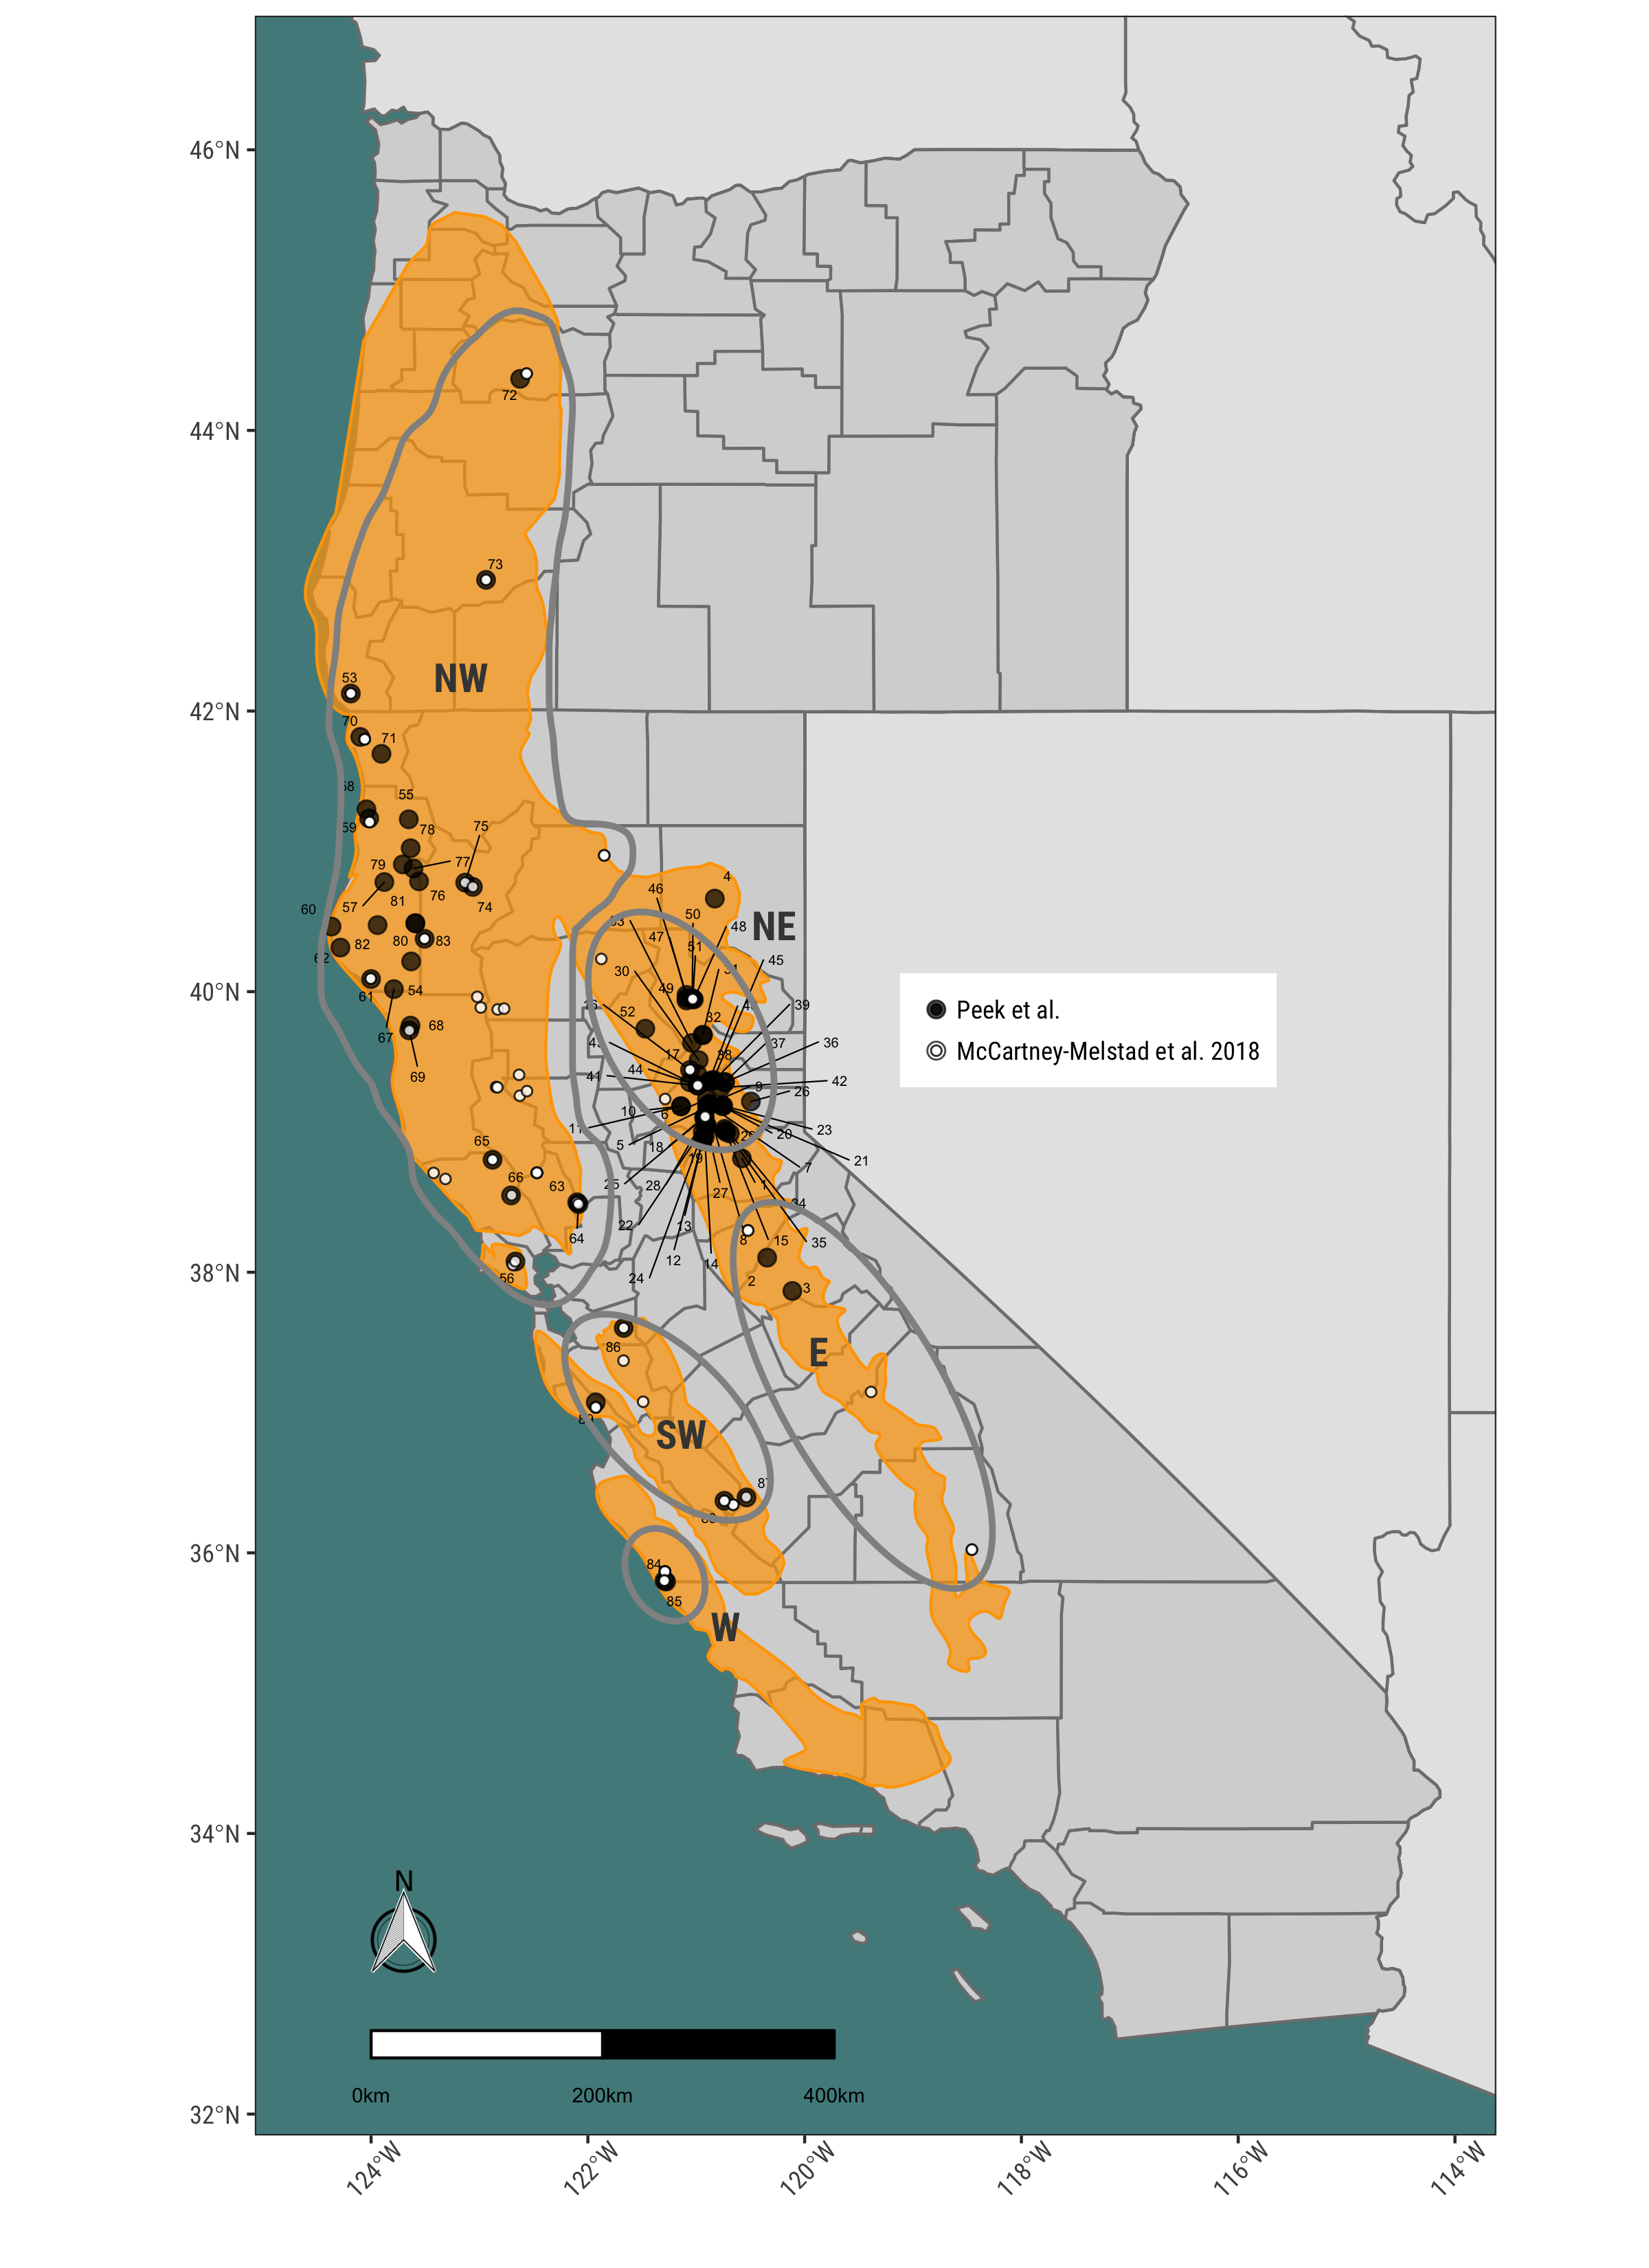
\includegraphics[width=0.85\linewidth]{figure/ch3/fig_01_maps_all_rabo_filt10_1_100k_revrange_localities_annotated} \caption{Map comparing sampling localities between the \emph{R.
boylii} study of McCartney-Melstad et al.
(\protect\hyperlink{ref-mccartney-melstad_population_2018}{2018}) and
the current study with a simplified historical range (yellow) of
\emph{R. boylii} (adapted from USFS 2011 and Thomson et al.
(\protect\hyperlink{ref-thomson_california_2016}{2016})). Clades
identified by McCartney-Melstad et al.
(\protect\hyperlink{ref-mccartney-melstad_population_2018}{2018}) are
circled.}\label{fig:CH3F1map}
\end{figure}
\clearpage

\begingroup\fontsize{8}{10}\selectfont
\begin{longtable}[t]{r>{\raggedright\arraybackslash}p{9em}llrrr>{\raggedright\arraybackslash}p{5em}>{\raggedright\arraybackslash}p{4em}}
\caption{\label{tab:CH3T1}Sampling Localities and clade groupings.}\\
\toprule
SiteID & Locality & River & Clade & Lat. & Lon. & HUC6 & County & n samples\\
\midrule
\endfirsthead
\caption[]{\label{tab:CH3T1}Sampling Localities and clade groupings. \textit{(continued)}}\\
\toprule
SiteID & Locality & River & Clade & Lat. & Lon. & HUC6 & County & n samples\\
\midrule
\endhead
\
\endfoot
\bottomrule
\endlastfoot
1 & SFA-CAMI & SFA & Unknown & 38.81151 & -120.5787 & 180201 & El Dorado & 6\\
2 & STAN-RoseCk & STAN & East & 38.10420 & -120.3460 & 180400 & Tuolumne & 2\\
3 & TUO-Clavey & TUO & East & 37.86643 & -120.1134 & 180400 & Tuolumne & 4\\
4 & ANTV-PineCk & ANTV & Unknown & 40.66316 & -120.8288 & 180800 & Lassen & 1\\
5 & BEAR & BEAR & North-East & 39.17484 & -120.8998 & 180201 & Nevada & 6\\
\addlinespace
6 & BEAR-GRHN & BEAR & North-East & 39.23206 & -120.9019 & 180201 & Nevada & 6\\
7 & BEAR-STH2 & BEAR & North-East & 39.19444 & -120.8878 & 180201 & Nevada & 6\\
8 & BEAR-STHA & BEAR & North-East & 39.18833 & -120.8981 & 180201 & Nevada & 3\\
9 & BEAR-STHC & BEAR & North-East & 39.20231 & -120.8754 & 180201 & Nevada & 10\\
10 & DEER-ClearCk & DEER & North-East & 39.18287 & -121.1410 & 180201 & Nevada & 3\\
\addlinespace
11 & DEER-CLEC & DEER & North-East & 39.18287 & -121.1410 & 180201 & Nevada & 2\\
12 & MFA-AMEC & MFA & North-East & 38.93396 & -120.9436 & 180201 & El Dorado & 6\\
13 & MFA-GASC & MFA & North-East & 38.96651 & -120.9325 & 180201 & Placer & 6\\
14 & MFA-TODC & MFA & North-East & 38.96385 & -120.9216 & 180201 & Placer & 9\\
15 & MFA-US-R & MFA & North-East & 39.00754 & -120.7316 & 180201 & Placer & 1\\
\addlinespace
16 & MFY-OREGCk & MFY & North-East & 39.44188 & -121.0575 & 180201 & Nevada & 10\\
17 & MFY-US-OH & MFY & North-East & 39.41305 & -120.9903 & 180201 & Nevada & 10\\
18 & NFA & NFA & North-East & 39.10722 & -120.9239 & 180201 & Placer & 10\\
19 & NFA-BUNC & NFA & North-East & 39.03762 & -120.9103 & 180201 & Placer & 10\\
20 & NFA-EUCHDS & NFA & North-East & 39.18492 & -120.7620 & 180201 & Placer & 5\\
\addlinespace
21 & NFA-EUCHUS & NFA & North-East & 39.18444 & -120.7505 & 180201 & Placer & 4\\
22 & NFA-INDC & NFA & North-East & 39.05665 & -120.9085 & 180201 & Placer & 10\\
23 & NFA-NFNFA & NFA & North-East & 39.18839 & -120.7592 & 180201 & Placer & 2\\
24 & NFA-POND & NFA & North-East & 38.99995 & -120.9406 & 180201 & Placer & 5\\
25 & NFA-ROBR & NFA & North-East & 39.10451 & -120.9267 & 180201 & Placer & 10\\
\addlinespace
26 & NFA-SAIC & NFA & North-East & 39.21694 & -120.4960 & 180201 & Placer & 5\\
27 & NFA-SHIC & NFA & North-East & 39.04073 & -120.9014 & 180201 & Placer & 10\\
28 & NFA-SLAR & NFA & North-East & 39.09865 & -120.9255 & 180201 & Placer & 8\\
29 & NFMFA-SC & NFMFA & North-East & 39.02237 & -120.7369 & 180201 & Placer & 10\\
30 & NFY & NFY & North-East & 39.51190 & -120.9774 & 180201 & Sierra & 10\\
\addlinespace
31 & NFY-SLATE & NFY & North-East & 39.69219 & -120.9399 & 180201 & Plumas & 1\\
32 & NFY-SLATE-CGRav & NFY & North-East & 39.68913 & -120.9389 & 180201 & Plumas & 3\\
33 & NFY-SLATE-Onion & NFY & North-East & 39.63414 & -121.0400 & 180201 & Plumas & 2\\
34 & RUB-LC-US & RUB & North-East & 38.98887 & -120.6900 & 180201 & Placer & 8\\
35 & RUB-USPH & RUB & North-East & 38.99928 & -120.7233 & 180201 & Placer & 10\\
\addlinespace
36 & SFY & SFY & North-East & 39.35386 & -120.7342 & 180201 & Nevada & 1\\
37 & SFY-FallCk & SFY & North-East & 39.35532 & -120.7370 & 180201 & Nevada & 5\\
38 & SFY-LOGA & SFY & North-East & 39.36914 & -120.8526 & 180201 & Nevada & 4\\
39 & SFY-MCKI & SFY & North-East & 39.36805 & -120.8354 & 180201 & Nevada & 2\\
40 & SFY-MISC & SFY & North-East & 39.36096 & -120.8814 & 180201 & Nevada & 6\\
\addlinespace
41 & SFY-RockCk & SFY & North-East & 39.32983 & -120.9863 & 180201 & Nevada & 3\\
42 & SFY-Scotchman & SFY & North-East & 39.31653 & -120.7733 & 180201 & Nevada & 2\\
43 & SFY-ShadyCk & SFY & North-East & 39.35433 & -121.0590 & 180201 & Nevada & 10\\
44 & SFY-SpringCk & SFY & North-East & 39.33233 & -120.9890 & 180201 & Nevada & 3\\
45 & SFY-THIMC & SFY & North-East & 39.36465 & -120.8462 & 180201 & Nevada & 1\\
\addlinespace
46 & FEA-BeanCk & FEA & North-East & 39.97650 & -121.0901 & 180201 & Plumas & 10\\
47 & FEA-SPANISH-BGulch & FEA & North-East & 39.95460 & -121.0887 & 180201 & Plumas & 6\\
48 & FEA-SPANISH-RockCk & FEA & North-East & 39.94449 & -121.0221 & 180201 & Plumas & 1\\
49 & FEA-SPANISH-SilverCk & FEA & North-East & 39.93733 & -121.0904 & 180201 & Plumas & 4\\
50 & FEA-SPANISH-Wapaunsie & FEA & North-East & 39.95226 & -121.0373 & 180201 & Plumas & 1\\
\addlinespace
51 & FEA-SpanishCk & FEA & North-East & 39.94637 & -121.0325 & 180201 & Plumas & 10\\
52 & NFF-Poe & NFF & North-East & 39.73598 & -121.4702 & 180201 & Butte & 4\\
53 & CHETCO-NookCk & CHETCO & North-West & 42.12500 & -124.1870 & 171003 & Curry & 1\\
54 & EEL & EEL & North-West & 40.21518 & -123.6303 & 180101 & Humboldt & 10\\
55 & KLAM-Aiken & KLAM & North-West & 41.22842 & -123.6524 & 180102 & Humboldt & 2\\
\addlinespace
56 & LAGUN-HalleckCk & LAGUN & North-West & 38.07650 & -122.6680 & 180500 & Marin & 1\\
57 & MAD-MapleCk & MAD & North-West & 40.78113 & -123.8778 & 180101 & Humboldt & 8\\
58 & MAD-RedwoodCk & MAD & North-West & 41.29934 & -124.0430 & 180101 & Humboldt & 9\\
59 & MAD-RedwoodCk2 & MAD & North-West & 41.23420 & -124.0171 & 180101 & Humboldt & 9\\
60 & MAT-BearRiver & MAT & North-West & 40.46383 & -124.3652 & 180101 & Humboldt & 9\\
\addlinespace
61 & MAT-HeadwaterMattole & MAT & North-West & 40.08992 & -124.0003 & 180101 & Humboldt & 1\\
62 & MAT-LowerMattole & MAT & North-West & 40.31408 & -124.2830 & 180101 & Humboldt & 5\\
63 & PUT-COLD & PUT & North-West & 38.49829 & -122.0988 & 180201 & Solano & 9\\
64 & PUT-WildhorseCk & PUT & North-West & 38.48616 & -122.0866 & 180201 & Solano & 10\\
65 & RUSS-HUNTCK & RUSS & North-West & 38.80166 & -122.8793 & 180101 & Sonoma & 1\\
\addlinespace
66 & RUSS-MWSprngCk & RUSS & North-West & 38.54757 & -122.7086 & 180101 & Sonoma & 10\\
67 & SFEEL & SFEEL & North-West & 40.01786 & -123.7896 & 180101 & Humboldt & 1\\
68 & SFEEL-Cedar & SFEEL & North-West & 39.75784 & -123.6364 & 180101 & Mendocino & 10\\
69 & SFEEL-Elder & SFEEL & North-West & 39.72383 & -123.6483 & 180101 & Mendocino & 2\\
70 & SMITH & SMITH & North-West & 41.81553 & -124.1003 & 180101 & Del Norte & 1\\
\addlinespace
71 & SMITH-HurdygurdyCk & SMITH & North-West & 41.69500 & -123.9043 & 180101 & Del Norte & 10\\
72 & SSANTIAM & SSANTIAM & North-West & 44.36750 & -122.6250 & 170900 & Linn & 7\\
73 & SUMPQUA & SUMPQUA & North-West & 42.93500 & -122.9390 & 171003 & Douglas & 2\\
74 & TRIN-ConnerCk & TRIN & North-West & 40.74656 & -123.0607 & 180102 & Trinity & 1\\
75 & TRIN-NFTrinity & TRIN & North-West & 40.77713 & -123.1318 & 180102 & Trinity & 1\\
\addlinespace
76 & TRIN-SFTrinity & TRIN & North-West & 40.78619 & -123.5575 & 180102 & Humboldt & 6\\
77 & TRIN-SFTrinity-SandyBar & TRIN & North-West & 40.87797 & -123.6088 & 180102 & Humboldt & 9\\
78 & TRIN-TishTang & TRIN & North-West & 41.02208 & -123.6351 & 180102 & Humboldt & 9\\
79 & TRIN-WillowCk & TRIN & North-West & 40.90705 & -123.7073 & 180102 & Humboldt & 1\\
80 & VANDZ-Dinsmore & VANDZ & North-West & 40.48759 & -123.5918 & 180101 & Humboldt & 9\\
\addlinespace
81 & VANDZ-Mill & VANDZ & North-West & 40.48759 & -123.5918 & 180101 & Humboldt & 1\\
82 & VANDZ-RootCreek & VANDZ & North-West & 40.47422 & -123.9400 & 180101 & Humboldt & 4\\
83 & VANDZ-Shanty & VANDZ & North-West & 40.37670 & -123.5061 & 180101 & Trinity & 3\\
84 & SANCARP-DutraCk & SANCARP & South-West & 35.80217 & -121.2932 & 180600 & Monterey & 10\\
85 & SANCARP-SanCarpoforoCk & SANCARP & South-West & 35.79533 & -121.2787 & 180600 & San Luis Obispo & 2\\
\addlinespace
86 & ALA-ArroyoMocho & ALA & West & 37.60299 & -121.6691 & 180500 & Alameda & 5\\
87 & DRY-Cantua\_AL & DRY & West & 36.39510 & -120.5359 & 180300 & Fresno & 1\\
88 & PAJ-ClearCk & PAJ & West & 36.37111 & -120.7400 & 180600 & San Benito & 3\\
89 & SOQUEL-EBSC & SOQUEL & West & 37.07300 & -121.9270 & 180600 & Santa Cruz & 10\\*
\end{longtable}\endgroup{}
\hypertarget{pca-and-admixture-shows-strong-separation-between-california-ecoregions}{%
\subsection{PCA and Admixture shows strong separation between California
ecoregions}\label{pca-and-admixture-shows-strong-separation-between-california-ecoregions}}

To compare and assess population structure patterns across the range of
\emph{R. boylii}, PCA were used to provide a dimensionless comparison of
genetic variation. The patterns of genetic differentiation largely
conformed to the clades described by McCartney-Melstad et al.
(\protect\hyperlink{ref-mccartney-melstad_population_2018}{2018})
(North-West {[}NW{]}, South-West {[}SW{]}, West {[}W{]},
North-East{[}NE{]}, and East {[}E{]}), but some notable differences were
observed. We used regional names for clades, thus the North Coast=NW,
the Central Coast=SW, the South Coast=W, the Northern Sierra=NE, the
Southern Sierra=E (Figure \ref{fig:CH3F2pca}). The main difference
evident in the PCA was the presence of a distinct group previously part
of the Northern Sierra, comprised of samples from the Feather basin.
Additional subdivision was evident in the Central/Southern coastal
region (two groups which match SW and W clades), and the Sierra Nevada
(two groups, matching the NE and E clades), yielding seven total
distinct structured groups. Interestingly, a small cluster of
individuals from the North Fork (NF) Feather River consistently
clustered along intermediate axes between the North Coast and Northern
Sierra/Southern Sierra groups. These individuals were consistently
intergrades between the larger Feather group and the Northern Coastal
group, regardless of the PC axes.

A single sampling locality from Lassen National Forest near Eagle Lake
(Locality 4, Table \ref{tab:CH3T1}) clustered with the Northern Sierra
group, suggesting the geographic boundary for this genetic group should
be extended (Figure \ref{fig:CH3F2pca}). Furthermore, individuals from
the South Fork (SF) American basin clustered with the Southern Sierra
(East) group, which would extend the boundary delineated by
McCartney-Melstad et al.
(\protect\hyperlink{ref-mccartney-melstad_population_2018}{2018}).

To assess how strongly the Feather and Southern/Central coastal samples
may have affected PCA structure, we ran several additional separate
post-hoc PCA analyses where all Feather samples were excluded, and all
Southern/Central coastal samples were excluded. Patterns remained
consistent with those observed when all samples were used (Figure
\ref{fig:CH3F2pca}), regardless of which samples were excluded or
retained. We conclude there is significant congruence with the
McCartney-Melstad et al.
(\protect\hyperlink{ref-mccartney-melstad_population_2018}{2018})
genetic clades, but an additional group appears distinct from the
original five delineated, the Feather watershed, and boundaries should
be expanded to include the SF American basin in the Southern Sierra, and
the Honey-Eagle Lakes basin in the Northern Sierra.









\begin{figure}

{\centering 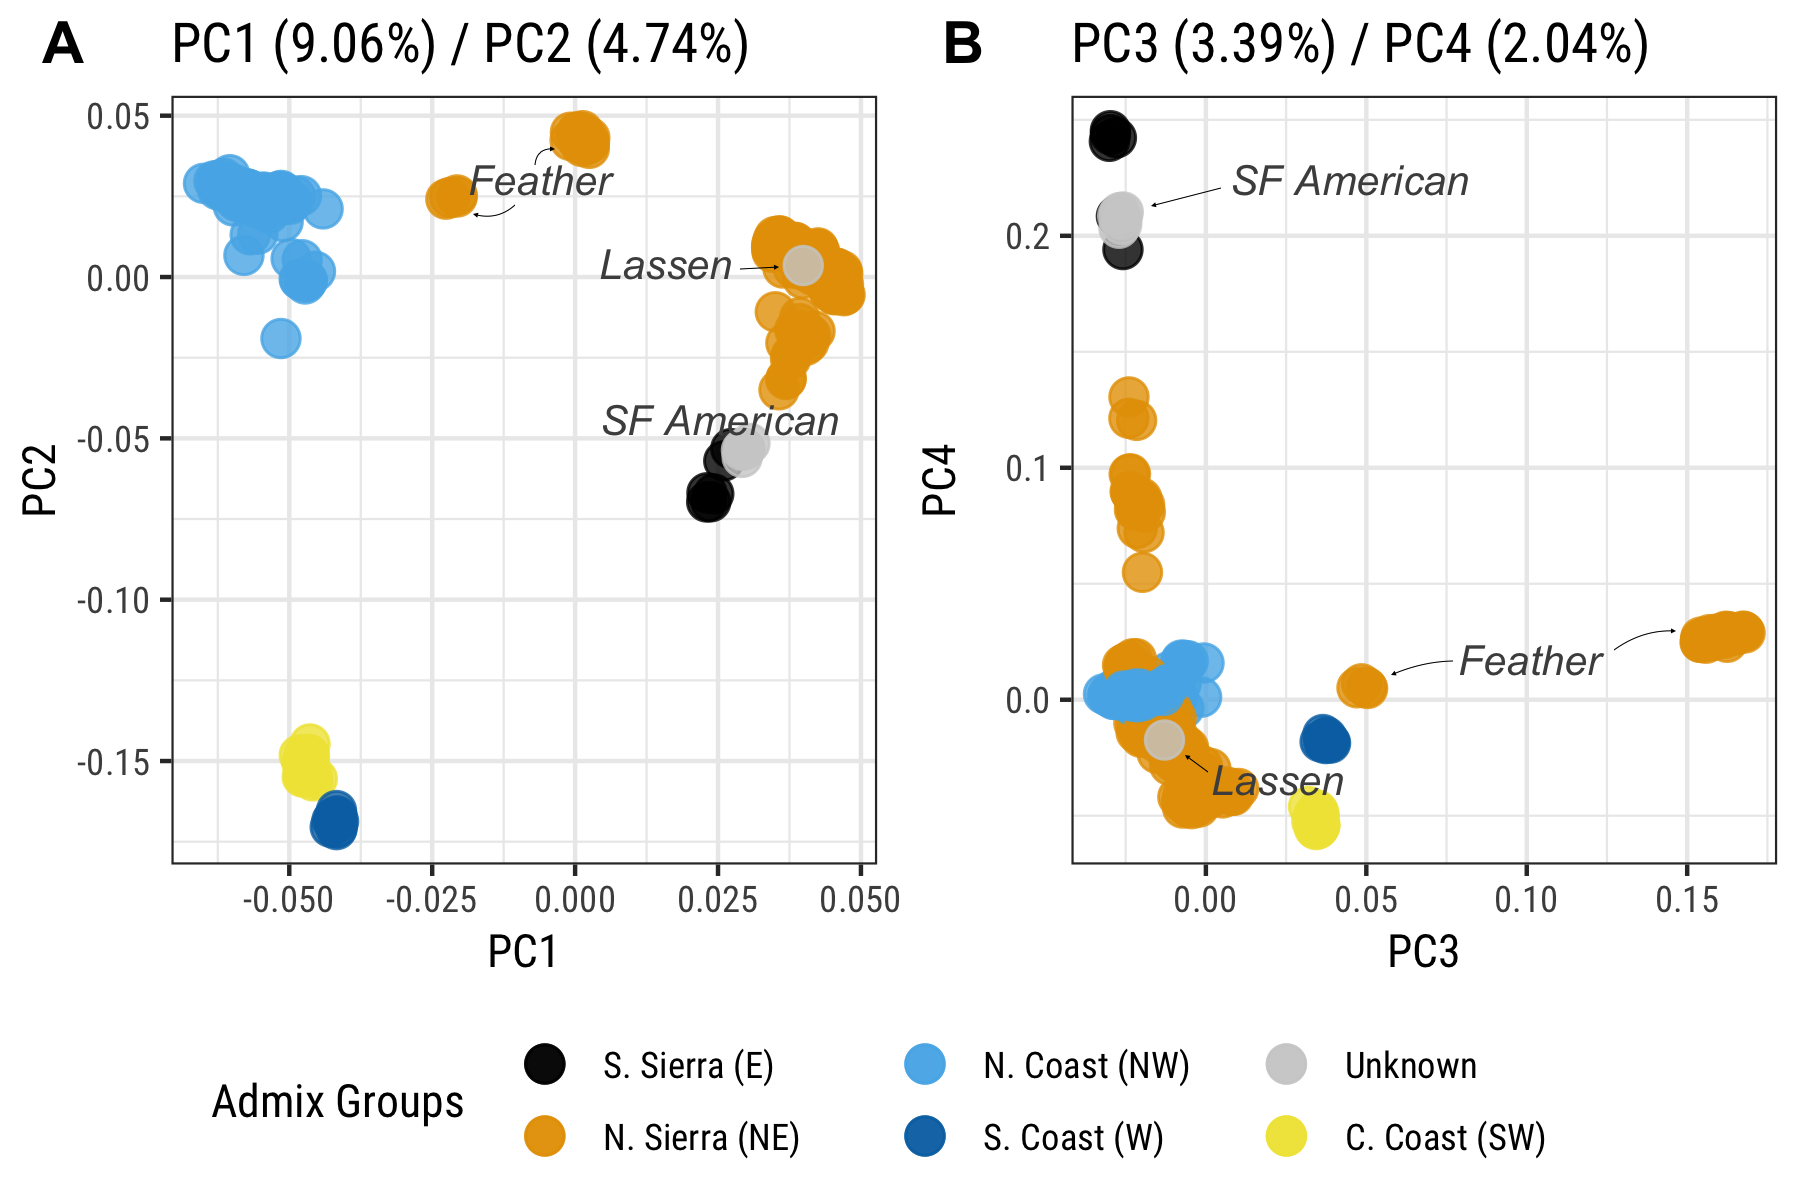
\includegraphics[width=0.95\linewidth]{figure/ch3/fig_02_pca_12_34_all_rabo_filt10_1_100k_thresh_annot} 

}

\caption{Principal component analysis of Rapture data colored by
genetic groups (in parentheses) from McCartney-Melstad et al.
(\protect\hyperlink{ref-mccartney-melstad_population_2018}{2018}). A)
PC1 vs.~PC2; B) PC3 vs.~PC4. Note, samples from South Fork American
River and Lassen County (gray) were not previously studied and thus had
no assigned clade. \emph{Rana boylii} in the Feather basin were assigned
as part of the Northern Sierra (NE) clade by McCartney-Melstad et al.
(\protect\hyperlink{ref-mccartney-melstad_population_2018}{2018}).}\label{fig:CH3F2pca}
\end{figure}
\clearpage

To further evaluate population structure across the range of \emph{R.
boylii}, we used NGSAdmix estimate the proportion of coancestry among
individuals (admixture) from genome-wide SNPs. We used a range of
k-values to evaluate the number of potential groups based on genetic
ancestry and found strong patterns of divergence which largely matched
the patterns observed in the PCA. While the northern and central coastal
(SW and W) groups showed strong divergence from all other groups, they
did not separate into distinct groups until k=9 (Figure
\ref{fig:CH3F3admix}). At k=3 through k=8, the N. Sierra and N. Coast
groups continued to show patterns of subdivision, while other groups
like the N. Sierra-Feather remained strongly distinct with little or no
admixture observed. At k=9, the Central Coast and South Coast split into
distinct groups, with additional patterns of substructure and admixture
observed in the N. Sierrae (NE) and the N. Coast (NW) groups (Figure 3).
While the Central/Southern Coastal populations are clearly distinct from
all other clades, our NGSadmix analysis of our data shows weaker support
for delineating Central (SW) and Southern (W) groups as distinct.





\begin{figure}

{\centering 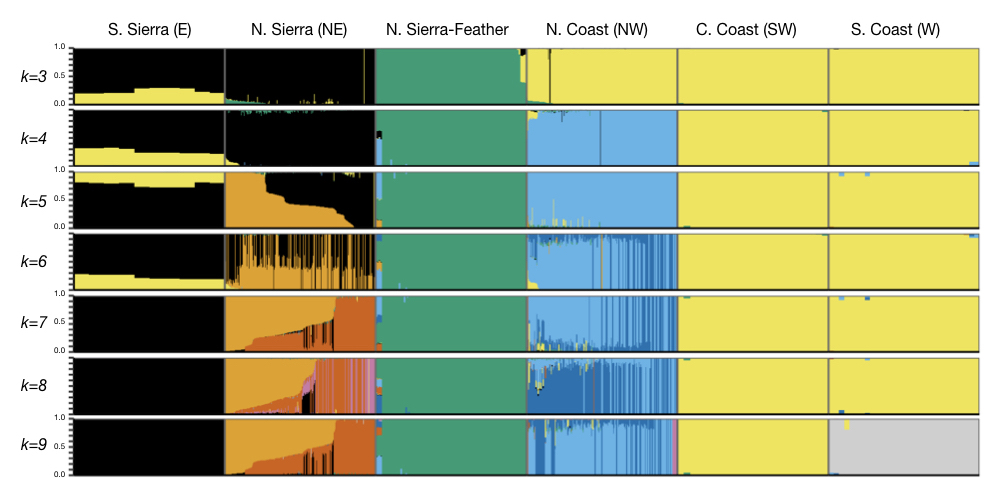
\includegraphics[width=0.95\linewidth]{figure/ch3/fig_03_admix_stacked_combined_rabo_filt_100k} 

}

\caption{NGSAdmixture for k=3 through k=9 for \emph{R. boylii}
across major geographic groupings (adapted from McCartney-Melstad et al.
(\protect\hyperlink{ref-mccartney-melstad_population_2018}{2018})). The
two Central/Southern Coastal groups did not differentiate until a k=9.}\label{fig:CH3F3admix}
\end{figure}
Sampling localities were then updated with genetic groups identified
from admixture and PCA analyses to delineate geographic boundaries for
these clades, building on McCartney-Melstad et al.
(\protect\hyperlink{ref-mccartney-melstad_population_2018}{2018})
(Figure \ref{fig:CH3F4map}). In summary, we identified \emph{R. boylii}
from the Feather Basin as a unique genetic group, the Southern Sierra
(East) clade should therefore extend to include the South Fork American
basin in El Dorado County (Locality 1), and the Northern Sierra
(North-East) clade should be expanded to include Honey-Eagle Lakes basin
in Lassen County (Locality 4, see Figure \ref{fig:CH3F1map} and Figure
\ref{fig:CH3F4map}).

\clearpage







\begin{figure}
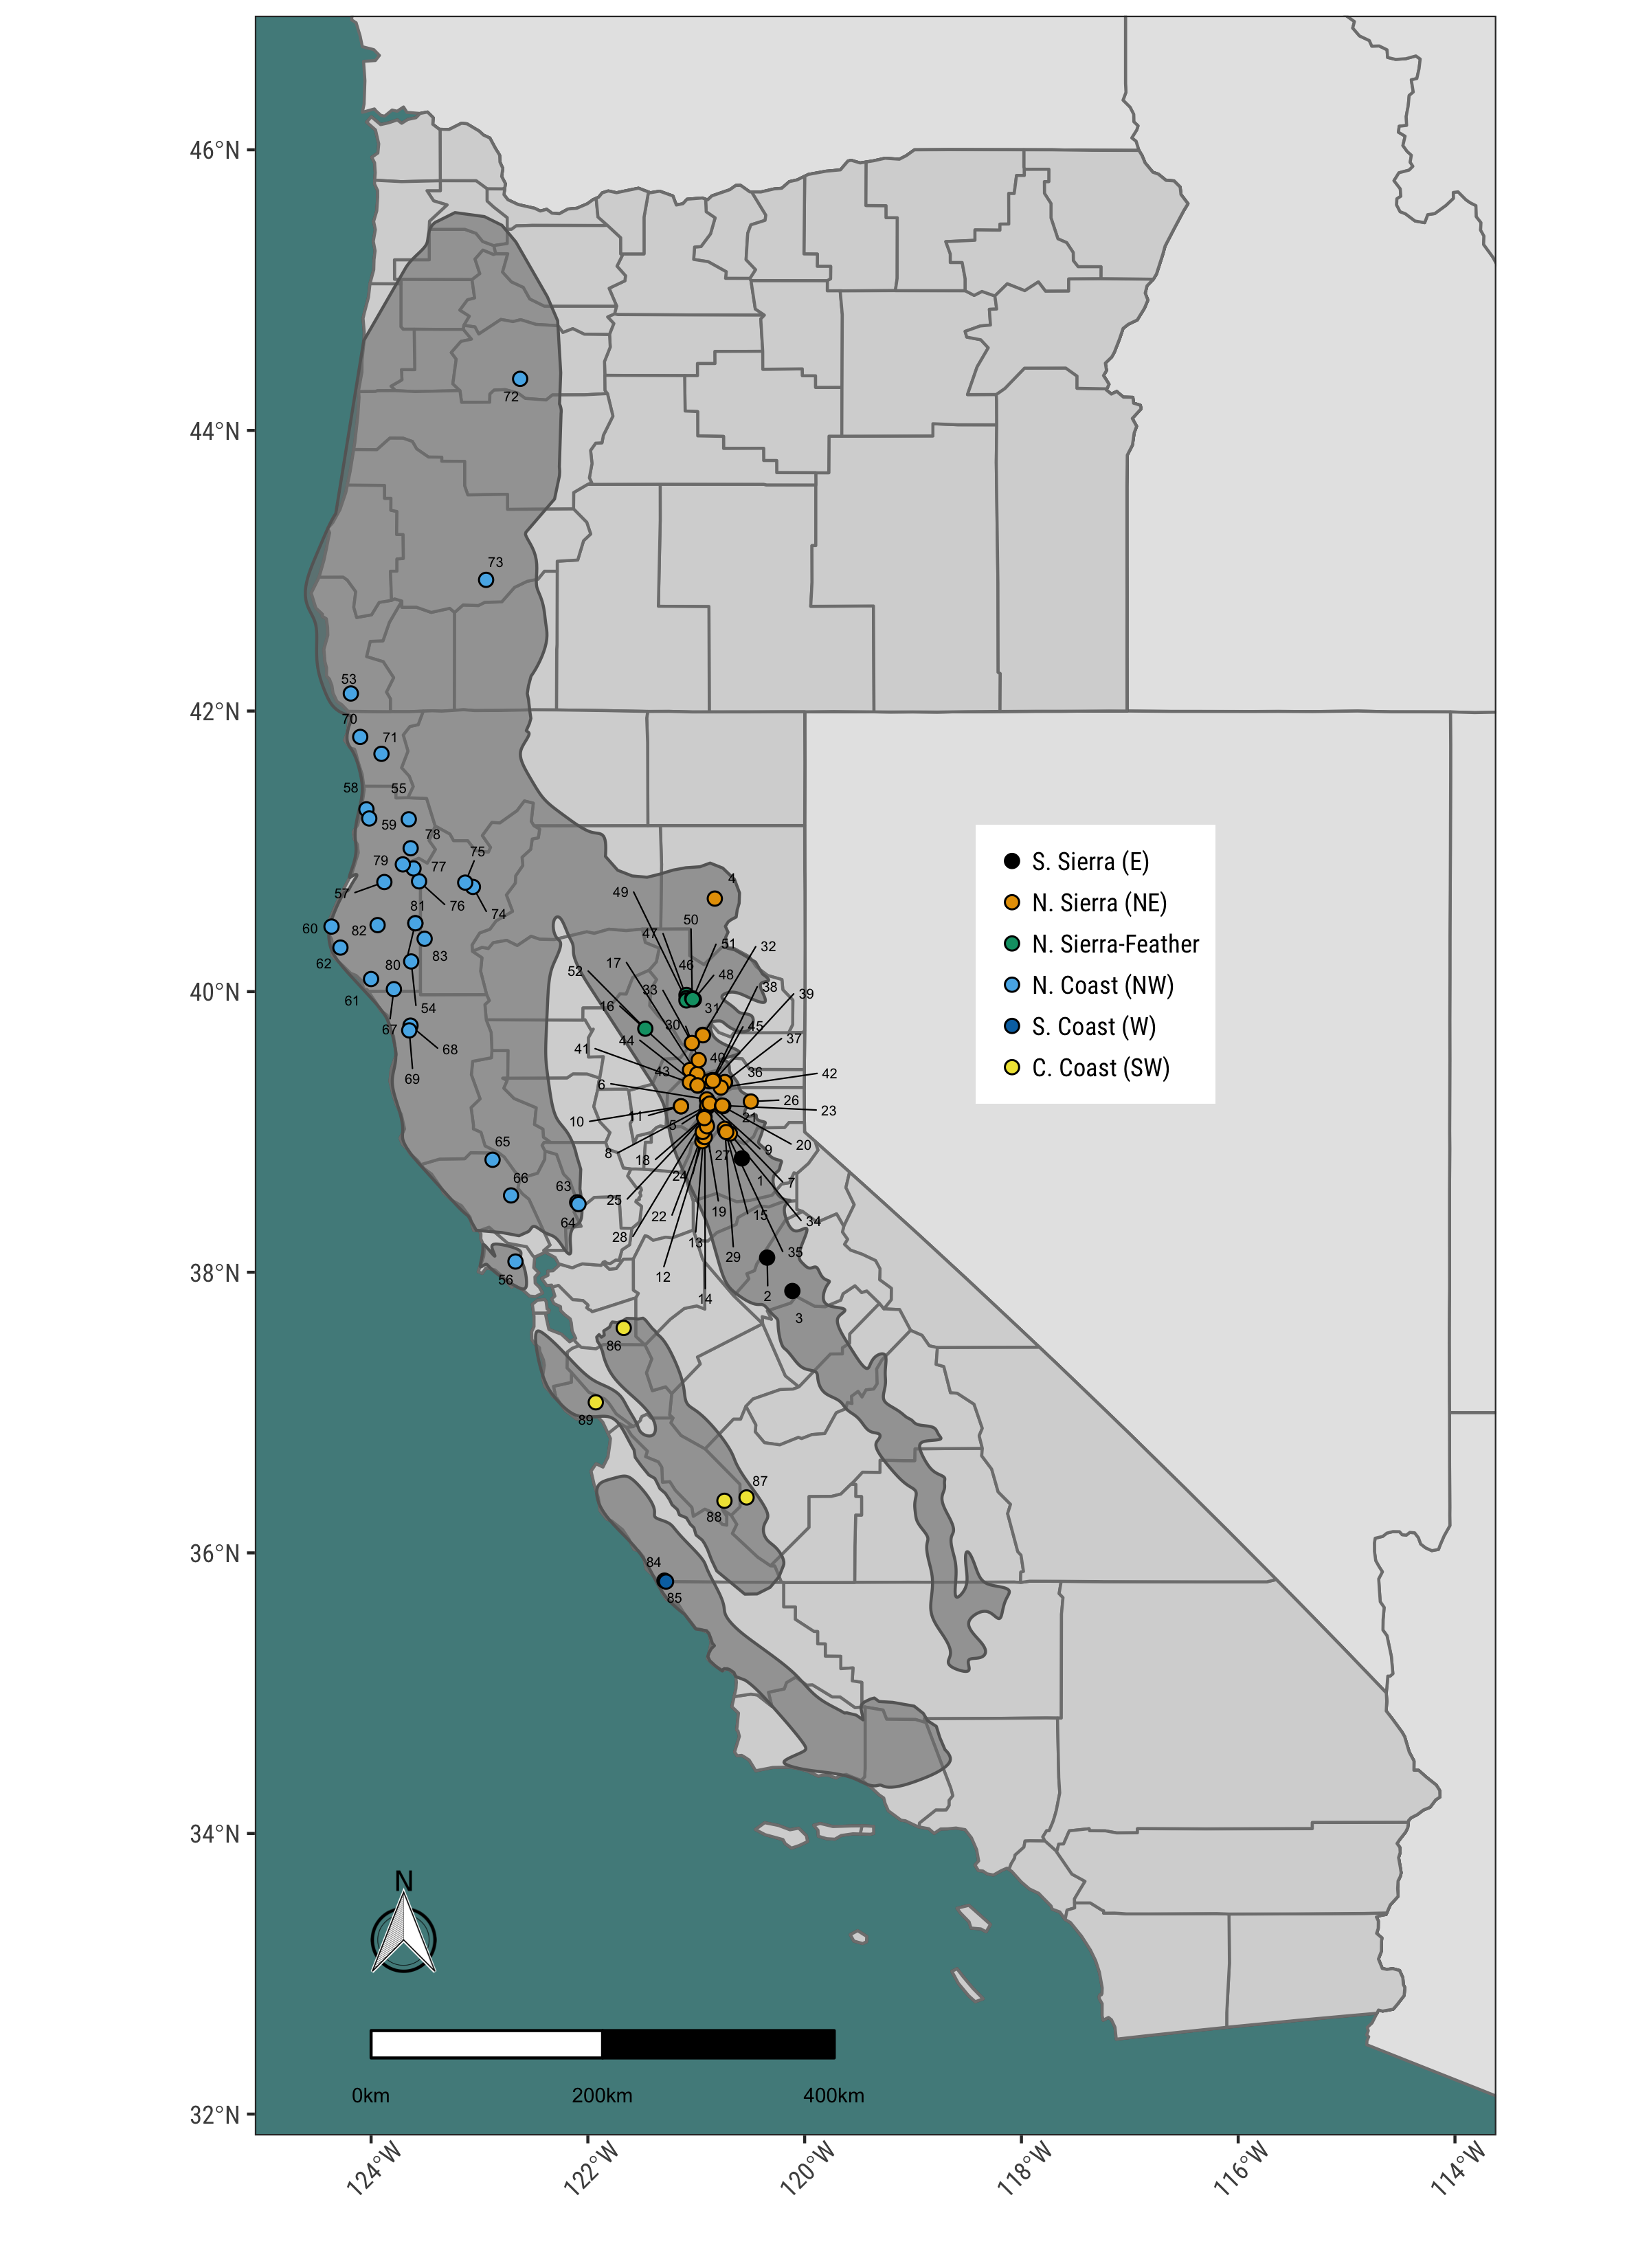
\includegraphics[width=0.85\linewidth]{figure/ch3/fig_04_maps_all_rabo_filt10_1_100k_clades_localities} \caption{Map of localities colored by genetic groupings. The
Northern Sierra-Feather group adds an additional genetically distinct
group, the Feather Basin to previous clades; Locality 1 extends the
boundary for the Southern Sierra (E) genetic clade up to the SF American
basin in El Dorado County, and Locality 4 extends the Northern Sierra
(NE) clade into Lassen County.}\label{fig:CH3F4map}
\end{figure}
\clearpage

\hypertarget{fst-shows-strong-divergence-across-regions}{%
\subsection{\texorpdfstring{F\textsubscript{ST} shows strong divergence
across
regions}{FST shows strong divergence across regions}}\label{fst-shows-strong-divergence-across-regions}}

To assess how distinct \emph{R. boylii} populations were across the
range of the species using F\textsubscript{ST} and genetic diversity
metrics, we selected all samples that had greater than 100,000
alignments from localities with at least three individuals, yielding a
total of 630 individuals from 63 localities for analysis (Table
\ref{tab:CH3T2}). Pairwise F\textsubscript{ST} was calculated between
each population pair (total combinations = 1,953), values ranged from 0
to 0.646. Extremely high F\textsubscript{ST} values were observed
between Central/South Coastal (SW/W) localities and all other localities
from other regions, indicating the coastal regions are strongly
divergent from \emph{R. boylii} in other parts of the species' range
(Figure \ref{fig:CH3F5fst}A). Comparison of pairwise F\textsubscript{ST}
values against geographic distance showed higher F\textsubscript{ST}
values between clades than within. Furthermore, the largest geographic
distances between locality pairs (i.e., between Southern Coastal
localities and Northern Coastal localities in Oregon) correlated with
higher F\textsubscript{ST} values. However, the highest
F\textsubscript{ST} values were not associated with the greatest
geographic distances, as the Sierra (NE/E) and Southern Coast (SW/W)
comparisons had the greatest pairwise F\textsubscript{ST} values
(\textgreater{} 0.6) of any pairwise comparison (Figure
\ref{fig:CH3F5fst}).

\par

\begingroup\fontsize{8}{10}\selectfont
\begin{longtable}[t]{r>{\raggedright\arraybackslash}p{9em}llrrr>{\raggedright\arraybackslash}p{5em}r}
\caption{\label{tab:CH3T2}Sampling localities with at least 3 individuals, used in population analyses of genetic diversity}\\
\toprule
SiteID & Locality & River & Clade & Lat. & Lon. & HUC6 & County & n samples\\
\midrule
\endfirsthead
\caption[]{\label{tab:CH3T2}Sampling localities with at least 3 individuals, used in population analyses of genetic diversity \textit{(continued)}}\\
\toprule
SiteID & Locality & River & Clade & Lat. & Lon. & HUC6 & County & n samples\\
\midrule
\endhead
\
\endfoot
\bottomrule
\endlastfoot
1 & SFA-CAMI & SFA & Unknown & 38.81151 & -120.5787 & 180201 & El Dorado & 6\\
2 & STAN-RoseCk & STAN & East & 38.10420 & -120.3460 & 180400 & Tuolumne & 2\\
3 & TUO-Clavey & TUO & East & 37.86643 & -120.1134 & 180400 & Tuolumne & 4\\
4 & ANTV-PineCk & ANTV & Unknown & 40.66316 & -120.8288 & 180800 & Lassen & 1\\
5 & BEAR & BEAR & North-East & 39.17484 & -120.8998 & 180201 & Nevada & 6\\
\addlinespace
6 & BEAR-GRHN & BEAR & North-East & 39.23206 & -120.9019 & 180201 & Nevada & 6\\
7 & BEAR-STH2 & BEAR & North-East & 39.19444 & -120.8878 & 180201 & Nevada & 6\\
8 & BEAR-STHA & BEAR & North-East & 39.18833 & -120.8981 & 180201 & Nevada & 3\\
9 & BEAR-STHC & BEAR & North-East & 39.20231 & -120.8754 & 180201 & Nevada & 10\\
10 & DEER-ClearCk & DEER & North-East & 39.18287 & -121.1410 & 180201 & Nevada & 3\\
\addlinespace
11 & DEER-CLEC & DEER & North-East & 39.18287 & -121.1410 & 180201 & Nevada & 2\\
12 & MFA-AMEC & MFA & North-East & 38.93396 & -120.9436 & 180201 & El Dorado & 6\\
13 & MFA-GASC & MFA & North-East & 38.96651 & -120.9325 & 180201 & Placer & 6\\
14 & MFA-TODC & MFA & North-East & 38.96385 & -120.9216 & 180201 & Placer & 9\\
15 & MFA-US-R & MFA & North-East & 39.00754 & -120.7316 & 180201 & Placer & 1\\
\addlinespace
16 & MFY-OREGCk & MFY & North-East & 39.44188 & -121.0575 & 180201 & Nevada & 10\\
17 & MFY-US-OH & MFY & North-East & 39.41305 & -120.9903 & 180201 & Nevada & 10\\
18 & NFA & NFA & North-East & 39.10722 & -120.9239 & 180201 & Placer & 10\\
19 & NFA-BUNC & NFA & North-East & 39.03762 & -120.9103 & 180201 & Placer & 10\\
20 & NFA-EUCHDS & NFA & North-East & 39.18492 & -120.7620 & 180201 & Placer & 5\\
\addlinespace
21 & NFA-EUCHUS & NFA & North-East & 39.18444 & -120.7505 & 180201 & Placer & 4\\
22 & NFA-INDC & NFA & North-East & 39.05665 & -120.9085 & 180201 & Placer & 10\\
23 & NFA-NFNFA & NFA & North-East & 39.18839 & -120.7592 & 180201 & Placer & 2\\
24 & NFA-POND & NFA & North-East & 38.99995 & -120.9406 & 180201 & Placer & 5\\
25 & NFA-ROBR & NFA & North-East & 39.10451 & -120.9267 & 180201 & Placer & 10\\
\addlinespace
26 & NFA-SAIC & NFA & North-East & 39.21694 & -120.4960 & 180201 & Placer & 5\\
27 & NFA-SHIC & NFA & North-East & 39.04073 & -120.9014 & 180201 & Placer & 10\\
28 & NFA-SLAR & NFA & North-East & 39.09865 & -120.9255 & 180201 & Placer & 8\\
29 & NFMFA-SC & NFMFA & North-East & 39.02237 & -120.7369 & 180201 & Placer & 10\\
30 & NFY & NFY & North-East & 39.51190 & -120.9774 & 180201 & Sierra & 10\\
\addlinespace
31 & NFY-SLATE & NFY & North-East & 39.69219 & -120.9399 & 180201 & Plumas & 1\\
32 & NFY-SLATE-CGRav & NFY & North-East & 39.68913 & -120.9389 & 180201 & Plumas & 3\\
33 & NFY-SLATE-Onion & NFY & North-East & 39.63414 & -121.0400 & 180201 & Plumas & 2\\
34 & RUB-LC-US & RUB & North-East & 38.98887 & -120.6900 & 180201 & Placer & 8\\
35 & RUB-USPH & RUB & North-East & 38.99928 & -120.7233 & 180201 & Placer & 10\\
\addlinespace
36 & SFY & SFY & North-East & 39.35386 & -120.7342 & 180201 & Nevada & 1\\
37 & SFY-FallCk & SFY & North-East & 39.35532 & -120.7370 & 180201 & Nevada & 5\\
38 & SFY-LOGA & SFY & North-East & 39.36914 & -120.8526 & 180201 & Nevada & 4\\
39 & SFY-MCKI & SFY & North-East & 39.36805 & -120.8354 & 180201 & Nevada & 2\\
40 & SFY-MISC & SFY & North-East & 39.36096 & -120.8814 & 180201 & Nevada & 6\\
\addlinespace
41 & SFY-RockCk & SFY & North-East & 39.32983 & -120.9863 & 180201 & Nevada & 3\\
42 & SFY-Scotchman & SFY & North-East & 39.31653 & -120.7733 & 180201 & Nevada & 2\\
43 & SFY-ShadyCk & SFY & North-East & 39.35433 & -121.0590 & 180201 & Nevada & 10\\
44 & SFY-SpringCk & SFY & North-East & 39.33233 & -120.9890 & 180201 & Nevada & 3\\
45 & SFY-THIMC & SFY & North-East & 39.36465 & -120.8462 & 180201 & Nevada & 1\\
\addlinespace
46 & FEA-BeanCk & FEA & North-East & 39.97650 & -121.0901 & 180201 & Plumas & 10\\
47 & FEA-SPANISH-BGulch & FEA & North-East & 39.95460 & -121.0887 & 180201 & Plumas & 6\\
48 & FEA-SPANISH-RockCk & FEA & North-East & 39.94449 & -121.0221 & 180201 & Plumas & 1\\
49 & FEA-SPANISH-SilverCk & FEA & North-East & 39.93733 & -121.0904 & 180201 & Plumas & 4\\
50 & FEA-SPANISH-Wapaunsie & FEA & North-East & 39.95226 & -121.0373 & 180201 & Plumas & 1\\
\addlinespace
51 & FEA-SpanishCk & FEA & North-East & 39.94637 & -121.0325 & 180201 & Plumas & 10\\
52 & NFF-Poe & NFF & North-East & 39.73598 & -121.4702 & 180201 & Butte & 4\\
53 & CHETCO-NookCk & CHETCO & North-West & 42.12500 & -124.1870 & 171003 & Curry & 1\\
54 & EEL & EEL & North-West & 40.21518 & -123.6303 & 180101 & Humboldt & 10\\
55 & KLAM-Aiken & KLAM & North-West & 41.22842 & -123.6524 & 180102 & Humboldt & 2\\
\addlinespace
56 & LAGUN-HalleckCk & LAGUN & North-West & 38.07650 & -122.6680 & 180500 & Marin & 1\\
57 & MAD-MapleCk & MAD & North-West & 40.78113 & -123.8778 & 180101 & Humboldt & 8\\
58 & MAD-RedwoodCk & MAD & North-West & 41.29934 & -124.0430 & 180101 & Humboldt & 9\\
59 & MAD-RedwoodCk2 & MAD & North-West & 41.23420 & -124.0171 & 180101 & Humboldt & 9\\
60 & MAT-BearRiver & MAT & North-West & 40.46383 & -124.3652 & 180101 & Humboldt & 9\\
\addlinespace
61 & MAT-HeadwaterMattole & MAT & North-West & 40.08992 & -124.0003 & 180101 & Humboldt & 1\\
62 & MAT-LowerMattole & MAT & North-West & 40.31408 & -124.2830 & 180101 & Humboldt & 5\\
63 & PUT-COLD & PUT & North-West & 38.49829 & -122.0988 & 180201 & Solano & 9\\
64 & PUT-WildhorseCk & PUT & North-West & 38.48616 & -122.0866 & 180201 & Solano & 10\\
65 & RUSS-HUNTCK & RUSS & North-West & 38.80166 & -122.8793 & 180101 & Sonoma & 1\\
\addlinespace
66 & RUSS-MWSprngCk & RUSS & North-West & 38.54757 & -122.7086 & 180101 & Sonoma & 10\\
67 & SFEEL & SFEEL & North-West & 40.01786 & -123.7896 & 180101 & Humboldt & 1\\
68 & SFEEL-Cedar & SFEEL & North-West & 39.75784 & -123.6364 & 180101 & Mendocino & 10\\
69 & SFEEL-Elder & SFEEL & North-West & 39.72383 & -123.6483 & 180101 & Mendocino & 2\\
70 & SMITH & SMITH & North-West & 41.81553 & -124.1003 & 180101 & Del Norte & 1\\
\addlinespace
71 & SMITH-HurdygurdyCk & SMITH & North-West & 41.69500 & -123.9043 & 180101 & Del Norte & 10\\
72 & SSANTIAM & SSANTIAM & North-West & 44.36750 & -122.6250 & 170900 & Linn & 7\\
73 & SUMPQUA & SUMPQUA & North-West & 42.93500 & -122.9390 & 171003 & Douglas & 2\\
74 & TRIN-ConnerCk & TRIN & North-West & 40.74656 & -123.0607 & 180102 & Trinity & 1\\
75 & TRIN-NFTrinity & TRIN & North-West & 40.77713 & -123.1318 & 180102 & Trinity & 1\\
\addlinespace
76 & TRIN-SFTrinity & TRIN & North-West & 40.78619 & -123.5575 & 180102 & Humboldt & 6\\
77 & TRIN-SFTrinity-SandyBar & TRIN & North-West & 40.87797 & -123.6088 & 180102 & Humboldt & 9\\
78 & TRIN-TishTang & TRIN & North-West & 41.02208 & -123.6351 & 180102 & Humboldt & 9\\
79 & TRIN-WillowCk & TRIN & North-West & 40.90705 & -123.7073 & 180102 & Humboldt & 1\\
80 & VANDZ-Dinsmore & VANDZ & North-West & 40.48759 & -123.5918 & 180101 & Humboldt & 9\\
\addlinespace
81 & VANDZ-Mill & VANDZ & North-West & 40.48759 & -123.5918 & 180101 & Humboldt & 1\\
82 & VANDZ-RootCreek & VANDZ & North-West & 40.47422 & -123.9400 & 180101 & Humboldt & 4\\
83 & VANDZ-Shanty & VANDZ & North-West & 40.37670 & -123.5061 & 180101 & Trinity & 3\\
84 & SANCARP-DutraCk & SANCARP & South-West & 35.80217 & -121.2932 & 180600 & Monterey & 10\\
85 & SANCARP-SanCarpoforoCk & SANCARP & South-West & 35.79533 & -121.2787 & 180600 & San Luis Obispo & 2\\
\addlinespace
86 & ALA-ArroyoMocho & ALA & West & 37.60299 & -121.6691 & 180500 & Alameda & 5\\
87 & DRY-Cantua\_AL & DRY & West & 36.39510 & -120.5359 & 180300 & Fresno & 1\\
88 & PAJ-ClearCk & PAJ & West & 36.37111 & -120.7400 & 180600 & San Benito & 3\\
89 & SOQUEL-EBSC & SOQUEL & West & 37.07300 & -121.9270 & 180600 & Santa Cruz & 10\\*
\end{longtable}\endgroup{}
\clearpage






\begin{figure}

{\centering 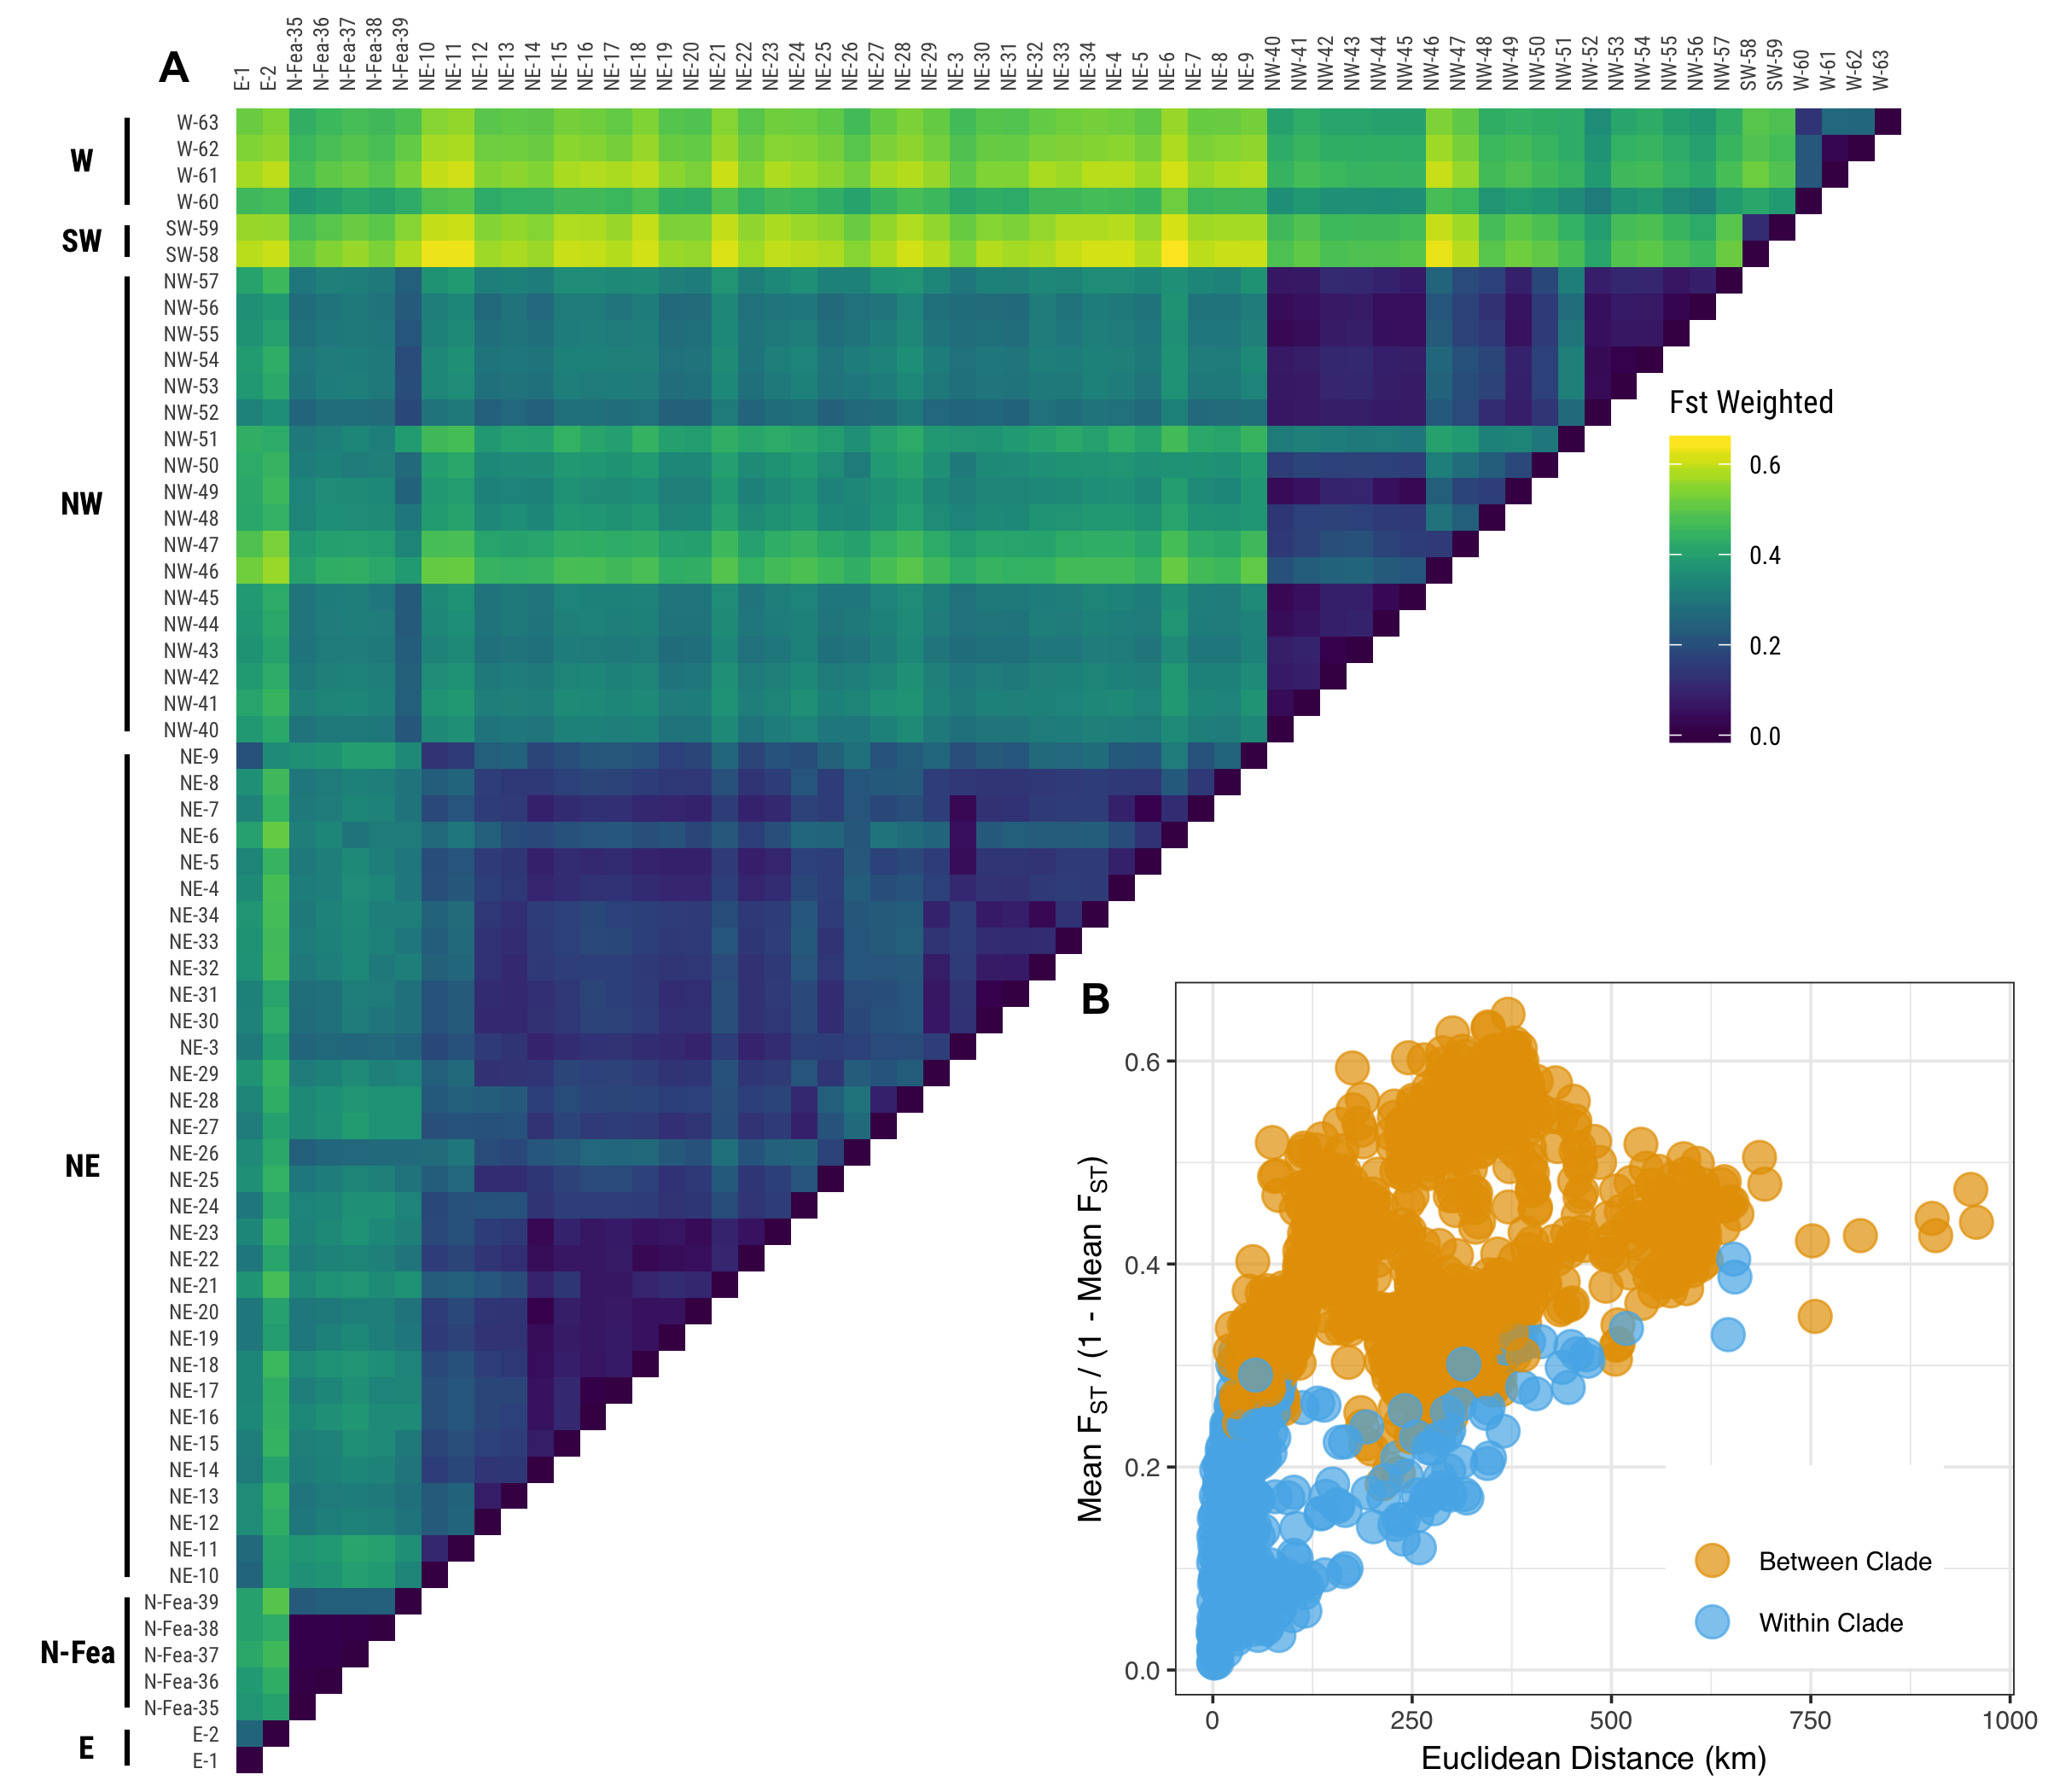
\includegraphics[width=0.95\linewidth]{figure/ch3/fig_05_combined_fst_cowplot_annotated} 

}

\caption{Plots of F\textsubscript{ST} for all localities sampled,
A) comparison of pairwise F\textsubscript{ST} for all localities grouped
by \emph{R. boylii} clades; and B) pairwise F\textsubscript{ST}
comparisons between and within clades vs.~geographic distance between
localities.}\label{fig:CH3F5fst}
\end{figure}
\clearpage

\hypertarget{genetic-variation-is-highest-in-the-north-west-and-lowest-in-the-east-south-west-clades}{%
\subsection{Genetic variation is highest in the North-West and lowest in
the East/ South-West
clades}\label{genetic-variation-is-highest-in-the-north-west-and-lowest-in-the-east-south-west-clades}}

Genetic diversity \(\theta\) estimates for each region showed \emph{R.
boylii} from the North Coast (NW) group had the greatest range in
genetic variation, with both the most diverse and least diverse
\(\theta\) estimates (Figure \ref{fig:CH3F6thetas}). Populations from
the Southern Sierra (E) and Central Coast (SW) had the lowest mean
Tajima's \(\theta_\pi\) (0.0064) and Watterson's \(\theta_W\) (0.0059 =
E, 0.0060 = SW), but both these groups had the lowest number of sampling
localities. The \(\Delta \theta\) was positive across all groups except
the North Coast, which exhibited the lowest value, while the Central
Coast (SW) and Southern Sierra (E) estimates were highest. Both coastal
groups (SW and W) had wide ranges of \(\Delta \theta\) estimates in
different locations. With the exception of the North Coast, which
contains the greatest genetic diversity and a trajectory of increasing
genetic diversity, overall genetic diversity data for \emph{R. boylii}
show a trajectory of genetic diversity loss, with many locations
exhibiting positive \(\Delta \theta\) (Figure \ref{fig:CH3F6thetas}D).








\begin{figure}

{\centering 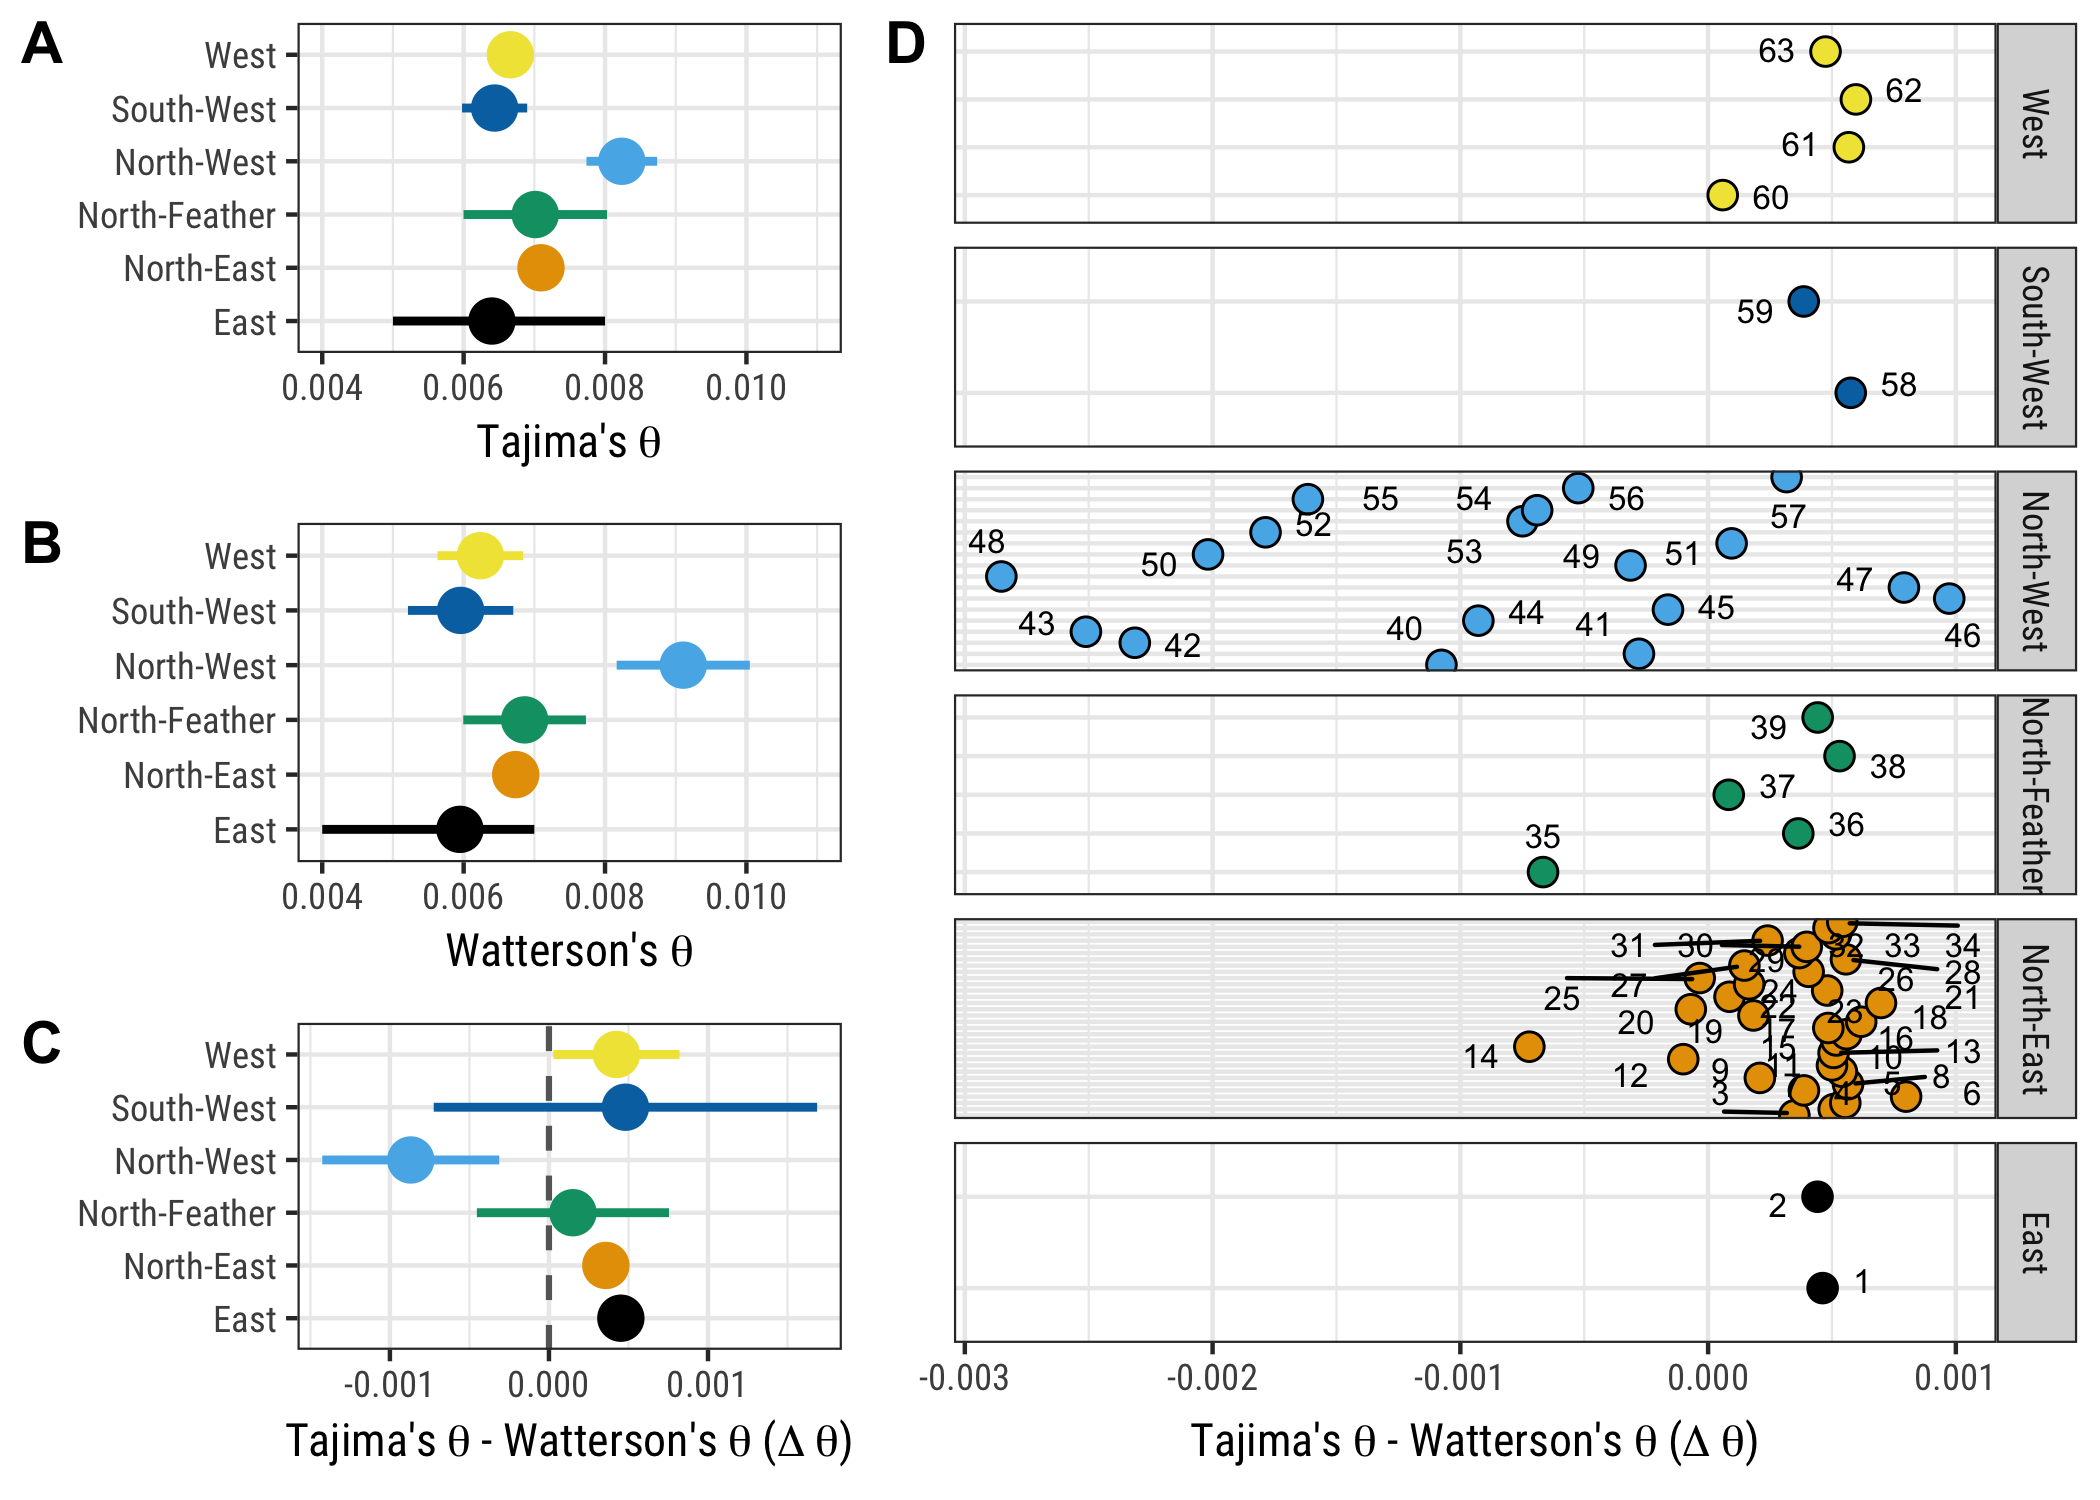
\includegraphics[width=0.95\linewidth]{figure/ch3/fig_06_thetas_taj_watt_tdiff_95CI_fig06} 

}

\caption{Tajima's \(\theta_\pi\) and Watterson' \(\theta_S\)
diversity estimates for \emph{R. boylii} by clade groups (adapted from
McCartney-Melstad et al.
(\protect\hyperlink{ref-mccartney-melstad_population_2018}{2018})) with
95\% CI. A) Tajima's \(\theta_\pi\)) by clade; B) Watterson'
\(\theta_S\) by clade; C) \(\theta_\pi - \theta_S\) aggregated by clade
and D) for each locality within clades.}\label{fig:CH3F6thetas}
\end{figure}
\clearpage

\hypertarget{discussion-and-conclusion}{%
\section{Discussion and Conclusion}\label{discussion-and-conclusion}}

As a species with a broad geographic range, \emph{Rana boylii} utilizes
a wide array of different landscapes throughout California and Oregon.
However, our study indicates there are strong patterns of geographic
structure and substantial differences in patterns of genetic diversity
across the species' range. The more comprehensive sampling provided by
this data set complements a recent genomic study of \emph{R. boylii}
(McCartney-Melstad et al.
\protect\hyperlink{ref-mccartney-melstad_population_2018}{2018}) and
largely supports the same clades identified using a different RADSeq
method. Moreover, our PCA and admixture results are congruent with the
five major clades identified in McCartney-Melstad et al.
(\protect\hyperlink{ref-mccartney-melstad_population_2018}{2018}), with
the exception of an additional novel group from the Feather watershed.
This congruence indicates these clades are important units which should
be considered carefully in planning conservation actions (i.e., such as
translocation, recolonization, and habitat restoration) for the species.

We also show that genetic data can provide resolution to prioritize
populations and regions at multiple scales. Evaluating the efficacy of
potential restoration actions can be difficult, particularly with rare
and cryptic species. Genetics provides a tool that can more effectively
track changes in population connectivity or genetic trajectories (i.e.,
low diversity, high F\textsubscript{ST}) which correspond to the
potential for long-term population persistence. Populations in the
Northern Coastal clade contained the greatest amount of genetic
variation, yet pairwise comparisons with populations from Central and
Southern Coast localities showed extremely high F\textsubscript{ST}
values, indicating these groups are genetically very distinct. In
addition, the Central/Southern Coast groups have relatively low genetic
diversity and trajectories of genetic diversity loss.

Recent sampling has largely occurred in the North Coast, Northern
Sierra, and Northern Sierra-Feather localities. The limited number of
sampling localities from the southern extent of the range of \emph{R.
boylii} correlates with population declines (Davidson
\protect\hyperlink{ref-davidson_declining_2004}{2004}, Adams et al.
\protect\hyperlink{ref-adams_rapid_2017}{2017}). Thus, conservation
actions should prioritize protecting sites in the Central/Southern Coast
and Southern Sierra clades, as these represent both the most genetically
divergent and distinct R. boylii, and simultaneously the most at-risk
populations. Extremely high F\textsubscript{ST} values between
populations from the same species as well as strong phylogeographic
structuring suggest limited gene flow through biogeographic barriers
(Spinks et al. \protect\hyperlink{ref-spinks_nuclear_2010}{2010},
Voelker et al. \protect\hyperlink{ref-voelker_river_2013}{2013}, Cazé et
al. \protect\hyperlink{ref-caze_could_2016}{2016}). This suggests
conservation management should consider these clades as distinct, and
future actions that include translocation or captive breeding should
utilize genetic data to assess potential impacts such as outbreeding
depression in locally adapted populations.

\emph{R. boylii} is an important sentinel stream species---not only as
link between both aquatic and riparian ecosystems---but also as a
sensitive gage of how altered hydrology affects riverine environments.
The impacts of regulated hydrology on \emph{R. boylii} populations have
been well documented (Kupferberg
\protect\hyperlink{ref-kupferberg_hydrologic_1996}{1996}, Lind et al.
\protect\hyperlink{ref-lind_effects_1996}{1996}, Yarnell et al.
\protect\hyperlink{ref-yarnell_dynamic_2012}{2012}, Kupferberg et al.
\protect\hyperlink{ref-kupferberg_effects_2012}{2012}, Catenazzi and
Kupferberg \protect\hyperlink{ref-catenazzi_importance_2013}{2013}). For
populations in regulated streams, genetic monitoring may be a crucial
component for assessing flow management actions on the probability of
long-term persistence (via maintenance of genetic diversity), as well as
tracking population responses (i.e., using metrics like
F\textsubscript{ST} and genetic diversity \(\theta\)) to restoration
actions.

\hypertarget{acknowledgements-1}{%
\subsection{Acknowledgements}\label{acknowledgements-1}}

Many thanks to all who helped collect/prepare samples: Corey Luna, Rick
Wachs, and Sarah Mussulman. This research could not have been conducted
without access to specimens from Brad Shaffer at the Krebb Museum at
UCLA, and field samples from Caren Goldberg and Mallory Bedwell at
Washington State University.

\appendix

\hypertarget{appendix-supplemental-tables-code}{%
\chapter{Appendix: Supplemental Tables \&
Code}\label{appendix-supplemental-tables-code}}

This includes repository links to supplementary tables and code for
analyses and figure generation.

\hypertarget{supptables}{%
\subsection{Supplemental Tables}\label{supptables}}
\begin{itemize}
\tightlist
\item
  Table S1: \protect\hyperlink{ch1samplecollection}{Chapter 1 Rapture
  Samples} can be found at:
  \begin{itemize}
  \tightlist
  \item
    \href{https://raw.githubusercontent.com/ryanpeek/peek_phd_supplemental_materials/master/supplemental_tables/S1_chap1_Rapture_samples.csv}{github.com/peek\_phd\_supplemental\_materials}
  \end{itemize}
\item
  Table S2: \protect\hyperlink{denovo}{RADSeq samples} used for
  designing baits can be found at:
  \begin{itemize}
  \tightlist
  \item
    \href{https://raw.githubusercontent.com/ryanpeek/peek_phd_supplemental_materials/master/supplemental_tables/S2_RADSeq-bait-samples.csv}{github.com/peek\_phd\_supplemental\_materials}
  \end{itemize}
\item
  Table S3: \protect\hyperlink{denovo}{\emph{de Novo}} alignment for
  \emph{R. boylii}. Zipped file is 4.16 MB and can be found at:
  \begin{itemize}
  \tightlist
  \item
    \href{https://github.com/ryanpeek/peek_phd_supplemental_materials/blob/master/supplemental_tables/S3_de_novo_assembly_300.fa.zip?raw=true}{github.com/peek\_phd\_supplemental\_materials}
  \end{itemize}
\item
  Table S4: \protect\hyperlink{rapture}{RAD Capture baits} can be found
  at:
  \begin{itemize}
  \tightlist
  \item
    \href{https://github.com/ryanpeek/peek_phd_supplemental_materials/blob/master/supplemental_tables/S4_capture_baits_120.fa.zip?raw=true}{github.com/peek\_phd\_supplemental\_materials}
  \end{itemize}
\item
  Table S5: \protect\hyperlink{ch2samplecollection}{Chapter 2 Hybrid
  Samples} can be found at:
  \begin{itemize}
  \tightlist
  \item
    \href{https://raw.githubusercontent.com/ryanpeek/peek_phd_supplemental_materials/master/supplemental_tables/S5_chap2_selected_samples_25k.csv}{github.com/peek\_phd\_supplemental\_materials}
  \end{itemize}
\end{itemize}
\hypertarget{code}{%
\subsection{Code}\label{code}}

The pipeline for analyses and associated code can be found at:
\begin{itemize}
\tightlist
\item
  \textbf{Miller Lab}: \url{https://github.com/miller-genetics-lab}
\item
  \url{https://ryanpeek.github.io/radseq/}
\end{itemize}
\hypertarget{colophon}{%
\chapter*{Colophon}\label{colophon}}
\addcontentsline{toc}{chapter}{Colophon}

This document is set in \href{https://github.com/georgd/EB-Garamond}{EB
Garamond}, \href{https://github.com/adobe-fonts/source-code-pro/}{Source
Code Pro} and \href{http://www.latofonts.com/lato-free-fonts/}{Lato}.
The body text is set at 11pt with \(\familydefault\).

It was written in R Markdown and \(\LaTeX\), and rendered into PDF using
\href{https://github.com/ryanpeek/ucd-aggiedown}{ucd-aggiedown} and
\href{https://github.com/rstudio/bookdown}{bookdown}, largely based on
the \href{https://github.com/benmarwick/huskydown}{huskydown} template.

This document was typeset using the XeTeX typesetting system, and the
University of California Thesis class (2012). The template meets
\href{https://grad.ucdavis.edu/resources/graduate-student-resources/academic-information-and-services/filing-thesis-or-dissertation}{UC
Davis Graduate Studies dissertation requirements as of Fall 2018} to
ensure that documents conform precisely to submission standards. Other
elements of the document formatting source code have been taken from the
\href{https://github.com/stevenpollack/ucbthesis}{Latex, Knitr, and
RMarkdown templates for UC Berkeley's graduate thesis}, and
\href{https://github.com/suchow/Dissertate}{Dissertate: a LaTeX
dissertation template to support the production and typesetting of a PhD
dissertation at Harvard, Princeton, and NYU}.

The source files for this thesis, along with data files are available at
\url{https://github.com/ryanpeek/peek_phd_supplemental_materials}.

This version of the thesis was generated on 2018-09-19 14:17:14.

\backmatter

\hypertarget{references}{%
\chapter*{References}\label{references}}
\addcontentsline{toc}{chapter}{References}

\markboth{References}{References}

\noindent

\setlength{\parindent}{-0.20in}
\setlength{\leftskip}{0.20in}
\setlength{\parskip}{8pt}

\hypertarget{refs}{}
\leavevmode\hypertarget{ref-abbott_hybridization_2013}{}%
Abbott, R., D. Albach, S. Ansell, J. W. Arntzen, S. J. E. Baird, N.
Bierne, J. Boughman, A. Brelsford, C. A. Buerkle, R. Buggs, R. K.
Butlin, U. Dieckmann, F. Eroukhmanoff, A. Grill, S. H. Cahan, J. S.
Hermansen, G. Hewitt, A. G. Hudson, C. Jiggins, J. Jones, B. Keller, T.
Marczewski, J. Mallet, P. Martinez-Rodriguez, M. Möst, S. Mullen, R.
Nichols, A. W. Nolte, C. Parisod, K. Pfennig, A. M. Rice, M. G. Ritchie,
B. Seifert, C. M. Smadja, R. Stelkens, J. M. Szymura, R. Väinölä, J. B.
W. Wolf, and D. Zinner. 2013. Hybridization and speciation. Journal of
evolutionary biology 26:229--246.

\leavevmode\hypertarget{ref-adams_rapid_2017}{}%
Adams, A. J., A. P. Pessier, and C. J. Briggs. 2017. Rapid extirpation
of a North American frog coincides with an increase in fungal pathogen
prevalence: Historical analysis and implications for reintroduction.
Ecology and evolution 7:10216--10232.

\leavevmode\hypertarget{ref-akaike_information_1973}{}%
Akaike, H. 1973. Information theory and an extension of the maximum
likelihood principle. Pages 267--281 \emph{in} B. N. Petrov and F.
Csaki, editors. Proceedings of the Second International Symposium on
Information Theory.

\leavevmode\hypertarget{ref-ali_rad_2016}{}%
Ali, O. A., S. M. O'Rourke, S. J. Amish, M. H. Meek, G. Luikart, C.
Jeffres, and M. R. Miller. 2016. RAD Capture (Rapture): Flexible and
Efficient Sequence-Based Genotyping. Genetics 202:389--400.

\leavevmode\hypertarget{ref-anderson_oceanic_2009}{}%
Anderson, J. J., and W. N. Beer. 2009. Oceanic, riverine, and genetic
influences on spring chinook salmon migration timing. Ecological
applications: a publication of the Ecological Society of America
19:1989--2003.

\leavevmode\hypertarget{ref-baird_rapid_2008}{}%
Baird, N. A., P. D. Etter, T. S. Atwood, M. C. Currey, A. L. Shiver, Z.
A. Lewis, E. U. Selker, W. A. Cresko, and E. A. Johnson. 2008. Rapid SNP
discovery and genetic mapping using sequenced RAD markers. PloS one
3:e3376.

\leavevmode\hypertarget{ref-baird_descriptions_1856}{}%
Baird, S. F. 1856. Descriptions of new genera and species of North
American Frogs. Pages 59--62 \emph{in} Proceedings of the Academy of
Natural Sciences of Philadelphia. Philadelphia, Academy of Natural
Sciences of Philadelphia.

\leavevmode\hypertarget{ref-barbosa_integrative_2018}{}%
Barbosa, S., F. Mestre, T. A. White, J. Paupério, P. C. Alves, and J. B.
Searle. 2018. Integrative approaches to guide conservation decisions:
Using genomics to define conservation units and functional corridors.
Molecular ecology.

\leavevmode\hypertarget{ref-barrera-guzman_hybrid_2018}{}%
Barrera-Guzmán, A. O., A. Aleixo, M. D. Shawkey, and J. T. Weir. 2018.
Hybrid speciation leads to novel male secondary sexual ornamentation of
an Amazonian bird. Proceedings of the National Academy of Sciences of
the United States of America 115:E218--E225.

\leavevmode\hypertarget{ref-beebee_amphibian_2005}{}%
Beebee, T. J. C., and R. A. Griffiths. 2005. The amphibian decline
crisis: A watershed for conservation biology? Biological conservation
125:271--285.

\leavevmode\hypertarget{ref-birkeland_pleistocene_1964}{}%
Birkeland, P. W. 1964. Pleistocene Glaciation of the Northern Sierra
Nevada, North of Lake Tahoe, California. The Journal of geology
72:810--825.

\leavevmode\hypertarget{ref-bondi_transferability_2013}{}%
Bondi, C. A., S. M. Yarnell, A. J. Lind, and A. Lind. 2013.
Transferability of habitat suitability criteria for a stream breeding
frog (\emph{Rana} \emph{Boylii}) in the Sierra Nevada, California.
Conservation and Biology 8:88--103.

\leavevmode\hypertarget{ref-botero_evolutionary_2015}{}%
Botero, C. A., F. J. Weissing, J. Wright, and D. R. Rubenstein. 2015.
Evolutionary tipping points in the capacity to adapt to environmental
change. Proceedings of the National Academy of Sciences of the United
States of America 112:184--189.

\leavevmode\hypertarget{ref-bourque_spatial_2008}{}%
Bourque, R. M. 2008, December. Spatial ecology of an inland population
of the Foothill yellow-legged frog (Rana boylii) in Tehama County,
California. PhD Thesis, Humboldt State University.

\leavevmode\hypertarget{ref-broquet_buccal_2007}{}%
Broquet, T., L. Berset-Braendli, G. Emaresi, and L. Fumagalli. 2007.
Buccal swabs allow efficient and reliable microsatellite genotyping in
amphibians. Conservation Genetics 8:509--511.

\leavevmode\hypertarget{ref-brown_predicting_2012}{}%
Brown, L. R., J. T. May, A. C. Rehn, P. R. Ode, I. R. Waite, and J. G.
Kennen. 2012. Predicting biological condition in southern California
streams. Landscape and urban planning 108:17--27.

\leavevmode\hypertarget{ref-bunn_basic_2002}{}%
Bunn, S. E., and A. H. Arthington. 2002. Basic principles and ecological
consequences of altered flow regimes for aquatic biodiversity.
Environmental management 30:492--507.

\leavevmode\hypertarget{ref-burkey_extinction_1989}{}%
Burkey, T. V. 1989. Extinction in Nature Reserves - the Effect of
Fragmentation and the Importance of Migration between Reserve Fragments.
Oikos 55:75--81.

\leavevmode\hypertarget{ref-camp_notes_1917}{}%
Camp, C. L. 1917. Notes on the systematic status of the toads and frogs
of California. University of California publications in zoology
17:115--125.

\leavevmode\hypertarget{ref-catenazzi_importance_2013}{}%
Catenazzi, A., and S. J. Kupferberg. 2013. The importance of thermal
conditions to recruitment success in stream-breeding frog populations
distributed across a productivity gradient. Biological Conservation
168:40--48.

\leavevmode\hypertarget{ref-caze_could_2016}{}%
Cazé, A. L. R., G. Mäder, T. S. Nunes, L. P. Queiroz, G. de Oliveira, J.
A. F. Diniz-Filho, S. L. Bonatto, and L. B. Freitas. 2016. Could refuge
theory and rivers acting as barriers explain the genetic variability
distribution in the Atlantic Forest? Molecular phylogenetics and
evolution 101:242--251.

\leavevmode\hypertarget{ref-davidson_declining_2004}{}%
Davidson, C. 2004. Declining downwind: Amphibian population declines in
california and historical pesticide use. Ecological Applications
14:1892--1902.

\leavevmode\hypertarget{ref-davidson_spatial_2002}{}%
Davidson, C., H. B. Shaffer, M. R. Jennings - Conservation Biology, and
2002. 2002. Spatial tests of the pesticide drift, habitat destruction,
UV-B, and climate-change hypotheses for California amphibian declines.
Conservation biology: the journal of the Society for Conservation
Biology 16:1588--1601.

\leavevmode\hypertarget{ref-death_boosted_2007}{}%
De'ath, G. 2007. Boosted trees for ecological modeling and prediction.
Ecology 88:243--251.

\leavevmode\hypertarget{ref-drost_collapse_1996}{}%
Drost, C. A., and G. M. Fellers. 1996. Collapse of a Regional Frog Fauna
in the Yosemite Area of the California Sierra Nevada, USA. Conservation
biology: the journal of the Society for Conservation Biology
10:414--425.

\leavevmode\hypertarget{ref-dudgeon_freshwater_2006}{}%
Dudgeon, D., A. H. Arthington, M. O. Gessner, Z.-I. Kawabata, D. J.
Knowler, C. Lévêque, R. J. Naiman, A.-H. Prieur-Richard, D. Soto, M. L.
J. Stiassny, and C. A. Sullivan. 2006. Freshwater biodiversity:
Importance, threats, status and conservation challenges. Biological
reviews of the Cambridge Philosophical Society 81:163--182.

\leavevmode\hypertarget{ref-durrell_geologic_1988}{}%
Durrell, C. 1988. Geologic History of the Feather River Country,
California. University of California Press.

\leavevmode\hypertarget{ref-excoffier_robust_2013}{}%
Excoffier, L., I. Dupanloup, E. Huerta-Sánchez, V. C. Sousa, and M.
Foll. 2013. Robust demographic inference from genomic and SNP data. PLoS
genetics 9:e1003905.

\leavevmode\hypertarget{ref-excoffier_fastsimcoal_2011}{}%
Excoffier, L., and M. Foll. 2011. Fastsimcoal: A continuous-time
coalescent simulator of genomic diversity under arbitrarily complex
evolutionary scenarios. Bioinformatics 27:1332--1334.

\leavevmode\hypertarget{ref-fahrig_habitat_1985}{}%
Fahrig, L., and G. Merriam. 1985. Habitat Patch Connectivity and
Population Survival. Ecology 66:1762--1768.

\leavevmode\hypertarget{ref-frankham_introduction_2002}{}%
Frankham, R. 2002. Introduction to Conservation Genetics. Cambridge
University Press, Cambridge, UK ; New York.

\leavevmode\hypertarget{ref-fuller_linking_2011}{}%
Fuller, T. E., K. L. Pope, D. T. Ashton, and H. H. Welsh. 2011. Linking
the Distribution of an Invasive Amphibian (Rana catesbeiana) to Habitat
Conditions in a Managed River System in Northern California. Restoration
Ecology 19:204--213.

\leavevmode\hypertarget{ref-fumagalli_quantifying_2013}{}%
Fumagalli, M., F. G. Vieira, T. S. Korneliussen, T. Linderoth, E.
Huerta-Sánchez, A. Albrechtsen, and R. Nielsen. 2013. Quantifying
population genetic differentiation from next-generation sequencing data.
Genetics 195:979--992.

\leavevmode\hypertarget{ref-fumagalli_ngstools_2014}{}%
Fumagalli, M., F. G. Vieira, T. Linderoth, and R. Nielsen. 2014.
ngsTools: Methods for population genetics analyses from next-generation
sequencing data. Bioinformatics 30:1486--1487.

\leavevmode\hypertarget{ref-gillespie_glaciations_2004}{}%
Gillespie, A. R., and P. H. Zehfuss. 2004. Glaciations of the Sierra
Nevada, California, USA. Pages 51--62 \emph{in} J. Ehlers and P. L.
Gibbard, editors. Developments in Quaternary Sciences. Elsevier.

\leavevmode\hypertarget{ref-gilpin_minimum_1986}{}%
Gilpin, M., and M. Soule. 1986. Minimum Viable Populations: Processes of
Species Extinction, Conservation Biology. Sunderland, Massachusetts:
Sin. Assoc.:19--34.

\leavevmode\hypertarget{ref-goldberg_frogs_2003}{}%
Goldberg, C. S., M. E. Kaplan, and C. R. Schwalbe. 2003. From the frog's
mouth: Buccal swabs for collection of DNA from amphibians.
Herpetological review 34:220--221.

\leavevmode\hypertarget{ref-graham_influence_2008}{}%
Graham, C. H., J. Elith, R. J. Hijmans, A. Guisan, A. Townsend Peterson,
B. A. Loiselle, and The Nceas Predicting Species Distributions Working
Group. 2008. The influence of spatial errors in species occurrence data
used in distribution models. The Journal of applied ecology 45:239--247.

\leavevmode\hypertarget{ref-grantham_climatic_2010}{}%
Grantham, T. E., A. M. Merenlender, and V. H. Resh. 2010. Climatic
influences and anthropogenic stressors: An integrated framework for
streamflow management in Mediterranean-climate California, USA.
Freshwater biology 55:188--204.

\leavevmode\hypertarget{ref-guisan_what_2007}{}%
Guisan, A., N. E. Zimmermann, J. Elith, C. H. Graham, S. Phillips, and
A. T. Peterson. 2007. What Matters for Predicting the Occurrences of
Trees: Techniques, Data, or Species' Characteristics? Ecological
monographs 77:615--630.

\leavevmode\hypertarget{ref-guzy_influence_2018}{}%
Guzy, J. C., E. A. Eskew, B. J. Halstead, and S. J. Price. 2018.
Influence of damming on anuran species richness in riparian areas: A
test of the serial discontinuity concept. Ecology and evolution.

\leavevmode\hypertarget{ref-hellsten_genome_2010}{}%
Hellsten, U., R. M. Harland, M. J. Gilchrist, D. Hendrix, J. Jurka, V.
Kapitonov, I. Ovcharenko, N. H. Putnam, S. Shu, L. Taher, I. L. Blitz,
B. Blumberg, D. S. Dichmann, I. Dubchak, E. Amaya, J. C. Detter, R.
Fletcher, D. S. Gerhard, D. Goodstein, T. Graves, I. V. Grigoriev, J.
Grimwood, T. Kawashima, E. Lindquist, S. M. Lucas, P. E. Mead, T.
Mitros, H. Ogino, Y. Ohta, A. V. Poliakov, N. Pollet, J. Robert, A.
Salamov, A. K. Sater, J. Schmutz, A. Terry, P. D. Vize, W. C. Warren, D.
Wells, A. Wills, R. K. Wilson, L. B. Zimmerman, A. M. Zorn, R. Grainger,
T. Grammer, M. K. Khokha, P. M. Richardson, and D. S. Rokhsar. 2010. The
genome of the Western clawed frog Xenopus tropicalis. Science
328:633--636.

\leavevmode\hypertarget{ref-hendricks_recent_2018}{}%
Hendricks, S., E. C. Anderson, T. Antao, L. Bernatchez, B. R. Forester,
B. Garner, B. K. Hand, P. A. Hohenlohe, M. Kardos, B. Koop, A.
Sethuraman, R. S. Waples, and G. Luikart. 2018. Recent advances in
conservation and population genomics data analysis. Evolutionary
applications.

\leavevmode\hypertarget{ref-heyer_measuring_1994}{}%
Heyer, W. R., M. A. Donnelly, R. W. McDiarmid, L.-A. C. Hayek, and M. S.
Foster. 1994. Measuring and monitoring biological diversity. Standard
methods for amphibians. Smithsonian Institution Press, Washington DC.

\leavevmode\hypertarget{ref-hijmans_dismo_2017}{}%
Hijmans, R. J., S. Phillips, J. Leathwick, and J. Elith. 2017. Dismo:
Species Distribution Modeling. R package.

\leavevmode\hypertarget{ref-hoffmann_climate_2011}{}%
Hoffmann, A. A., and C. M. Sgrò. 2011. Climate change and evolutionary
adaptation. Nature 470:479--485.

\leavevmode\hypertarget{ref-hotaling_demographic_2018}{}%
Hotaling, S., C. C. Muhlfeld, J. J. Giersch, O. A. Ali, S. Jordan, M. R.
Miller, G. Luikart, and D. W. Weisrock. 2018. Demographic modelling
reveals a history of divergence with gene flow for a glacially tied
stonefly in a changing post-Pleistocene landscape. Journal of
biogeography 45:304--317.

\leavevmode\hypertarget{ref-ishiyama_differential_2015}{}%
Ishiyama, N., I. Koizumi, T. Yuta, and F. Nakamura. 2015. Differential
effects of spatial network structure and scale on population size and
genetic diversity of the ninespine stickleback in a remnant wetland
system. Freshwater biology 60:733--744.

\leavevmode\hypertarget{ref-jennings_amphibian_1994}{}%
Jennings, M. R., and M. P. Hayes. 1994. Amphibian and reptile species of
special concern in California. Final Report. California Department of
Fish and Game Inland Fisheries Division, Rancho Cordova.

\leavevmode\hypertarget{ref-kahilainen_conservation_2014}{}%
Kahilainen, A., M. Puurtinen, and J. S. Kotiaho. 2014. Conservation
implications of speciesGenetic diversity correlations. Global Ecology
and Conservation 2:315--323.

\leavevmode\hypertarget{ref-kim_estimation_2011}{}%
Kim, S. Y., K. E. Lohmueller, A. Albrechtsen, Y. Li, T. Korneliussen, G.
Tian, N. Grarup, T. Jiang, G. Andersen, D. Witte, T. Jorgensen, T.
Hansen, O. Pedersen, J. Wang, and R. Nielsen. 2011. Estimation of allele
frequency and association mapping using next-generation sequencing data.
BMC bioinformatics 12:231.

\leavevmode\hypertarget{ref-knapp_large-scale_2016}{}%
Knapp, R. A., G. M. Fellers, P. M. Kleeman, D. A. W. Miller, V. T.
Vredenburg, E. B. Rosenblum, and C. J. Briggs. 2016. Large-scale
recovery of an endangered amphibian despite ongoing exposure to multiple
stressors. Proceedings of the National Academy of Sciences of the United
States of America 113:11889--11894.

\leavevmode\hypertarget{ref-knapp_developing_2003}{}%
Knapp, R., K. Matthews, H. Preisler, and R. Jellison. 2003. Developing
probabilistic models to predict amphibian site occupancy in a patchy
landscape. Ecological applications: a publication of the Ecological
Society of America 13:1069--1082.

\leavevmode\hypertarget{ref-korneliussen_angsd_2014}{}%
Korneliussen, T. S., A. Albrechtsen, and R. Nielsen. 2014. ANGSD:
Analysis of Next Generation Sequencing Data. BMC bioinformatics 15:356.

\leavevmode\hypertarget{ref-korneliussen_calculation_2013}{}%
Korneliussen, T. S., I. Moltke, A. Albrechtsen, and R. Nielsen. 2013.
Calculation of Tajima's D and other neutrality test statistics from low
depth next-generation sequencing data. BMC bioinformatics 14:289.

\leavevmode\hypertarget{ref-krohn_conservation_2018}{}%
Krohn, A. R., C. J. Conroy, R. Pesapane, K. Bi, J. E. Foley, and E. B.
Rosenblum. 2018. Conservation genomics of desert dwelling California
voles (Microtus californicus) and implications for management of
endangered Amargosa voles (Microtus californicus scirpensis).
Conservation genetics 19:383--395.

\leavevmode\hypertarget{ref-kupferberg_hydrologic_1996}{}%
Kupferberg, S. J. 1996. Hydrologic and geomorphic factors affecting
conservation of a river-breeding frog (Rana boylii). Ecological
applications: a publication of the Ecological Society of America
6:1332--1344.

\leavevmode\hypertarget{ref-kupferberg_effects_2012}{}%
Kupferberg, S. J., W. J. Palen, A. J. Lind, S. Bobzien, A. Catenazzi, J.
Drennan, and M. E. Power. 2012. Effects of flow regimes altered by dams
on survival, population declines, and range-wide losses of California
river-breeding frogs. Conservation biology: the journal of the Society
for Conservation Biology 26:513--524.

\leavevmode\hypertarget{ref-kupferberg_pulsed_2009}{}%
Kupferberg, S., A. Lind, J. Mount, and S. Yarnell. 2009. Pulsed flow
effects on the Foothill Yellow- Legged Frog (Rana boylii): Integration
of empirical, experimental, and hydrodynamic modeling approaches.
California Energy Commission, PIER.

\leavevmode\hypertarget{ref-lande_role_1996}{}%
Lande, R., and S. Shannon. 1996. The Role of Genetic Variation in
Adaptation and Population Persistence in a Changing Environment.
Evolution; International Journal of Organic Evolution 50:434--437.

\leavevmode\hypertarget{ref-li_statistical_2011}{}%
Li, H. 2011. A statistical framework for SNP calling, mutation
discovery, association mapping and population genetical parameter
estimation from sequencing data. Bioinformatics 27:2987--2993.

\leavevmode\hypertarget{ref-li_aligning_2013}{}%
Li, H. 2013. Aligning sequence reads, clone sequences and assembly
contigs with BWA-MEM.

\leavevmode\hypertarget{ref-li_fast_2010}{}%
Li, H., and R. Durbin. 2010. Fast and accurate long-read alignment with
Burrows-Wheeler transform. Bioinformatics 26:589--595.

\leavevmode\hypertarget{ref-li_inference_2011}{}%
Li, H., and R. Durbin. 2011. Inference of human population history from
individual whole-genome sequences. Nature 475:493--496.

\leavevmode\hypertarget{ref-li_sequence_2009}{}%
Li, H., B. Handsaker, A. Wysoker, T. Fennell, J. Ruan, N. Homer, G.
Marth, G. Abecasis, R. Durbin, and 1000 Genome Project Data Processing
Subgroup. 2009. The Sequence Alignment/Map format and SAMtools.
Bioinformatics 25:2078--2079.

\leavevmode\hypertarget{ref-li_ten_2017}{}%
Li, Y., X.-X. Zhang, R.-L. Mao, J. Yang, C.-Y. Miao, Z. Li, and Y.-X.
Qiu. 2017. Ten Years of Landscape Genomics: Challenges and
Opportunities. Frontiers in plant science 8:2136.

\leavevmode\hypertarget{ref-lind_effects_1996}{}%
Lind, A. J., H. H. Welsh Jr, and R. A. Wilson. 1996. The effects of a
dam on breeding habitat and egg survival of the foothill yellow-legged
frog (Rana boylii) in Northwestern Calfifornia. Herpetological review
27:62--66.

\leavevmode\hypertarget{ref-macey_molecular_2001}{}%
Macey, J. R., J. L. Strasburg, J. A. Brisson, V. T. Vredenburg, M.
Jennings, and A. Larson. 2001. Molecular phylogenetics of western North
American frogs of the Rana boylii species group. Molecular phylogenetics
and evolution 19:131--143.

\leavevmode\hypertarget{ref-mallet_hybrid_2007}{}%
Mallet, J. 2007. Hybrid speciation. Nature 446:279--283.

\leavevmode\hypertarget{ref-malone_patterns_2008}{}%
Malone, J. H., and B. E. Fontenot. 2008. Patterns of reproductive
isolation in toads. PloS one 3:e3900.

\leavevmode\hypertarget{ref-mccartney-melstad_population_2018}{}%
McCartney-Melstad, E., M. Gidiş, and H. B. Shaffer. 2018. Population
genomic data reveal extreme geographic subdivision and novel
conservation actions for the declining foothill yellow-legged frog.
Heredity.

\leavevmode\hypertarget{ref-miller_conserved_2012}{}%
Miller, M. R., J. P. Brunelli, P. A. Wheeler, S. Liu, C. E. Rexroad 3rd,
Y. Palti, C. Q. Doe, and G. H. Thorgaard. 2012. A conserved haplotype
controls parallel adaptation in geographically distant salmonid
populations. Molecular ecology 21:237--249.

\leavevmode\hypertarget{ref-miller_rapid_2007}{}%
Miller, M. R., J. P. Dunham, A. Amores, W. A. Cresko, and E. A. Johnson.
2007. Rapid and cost-effective polymorphism identification and
genotyping using restriction site associated DNA (RAD) markers. Genome
Research 17:240--248.

\leavevmode\hypertarget{ref-monsen_extreme_2004}{}%
Monsen, K. J., and M. S. Blouin. 2004. Extreme isolation by distance in
a montane frog Rana cascadae. Conservation genetics 5:827--835.

\leavevmode\hypertarget{ref-moore_rangewide_2013}{}%
Moore, J. G., and B. C. Moring. 2013. Rangewide glaciation in the Sierra
Nevada, California. Geosphere 9:1804--1818.

\leavevmode\hypertarget{ref-moyle_rapid_2011}{}%
Moyle, P. B., J. V. E. Katz, and R. M. Quiñones. 2011. Rapid decline of
California's native inland fishes: A status assessment. Biological
conservation 144:2414--2423.

\leavevmode\hypertarget{ref-murchie_fish_2008}{}%
Murchie, K. J., K. P. E. Hair, C. E. Pullen, T. D. Redpath, H. R.
Stephens, and S. J. Cooke. 2008. Fish response to modified flow regimes
in regulated rivers: Research methods, effects and opportunities. River
research and applications 24:197--217.

\leavevmode\hypertarget{ref-narum_genotyping-by-sequencing_2013}{}%
Narum, S. R., C. A. Buerkle, J. W. Davey, M. R. Miller, and P. A.
Hohenlohe. 2013. Genotyping-by-sequencing in ecological and conservation
genomics. Molecular Ecology 22:2841--2847.

\leavevmode\hypertarget{ref-nielsen_snp_2012}{}%
Nielsen, R., T. Korneliussen, A. Albrechtsen, Y. Li, and J. Wang. 2012.
SNP calling, genotype calling, and sample allele frequency estimation
from New-Generation Sequencing data. PloS one 7:e37558.

\leavevmode\hypertarget{ref-nilsson_fragmentation_2005}{}%
Nilsson, C., C. A. Reidy, M. Dynesius, and C. Revenga. 2005.
Fragmentation and flow regulation of the world's large river systems.
Science 308:405--408.

\leavevmode\hypertarget{ref-nunziata_genomic_2017}{}%
Nunziata, S. O., S. L. Lance, D. E. Scott, E. M. Lemmon, and D. W.
Weisrock. 2017. Genomic data detect corresponding signatures of
population size change on an ecological time scale in two salamander
species. Molecular ecology 26:1060--1074.

\leavevmode\hypertarget{ref-pagano_frog_2003}{}%
Pagano, A., A. Dubois, D. Lesbarrères, and T. Lodé. 2003. Frog alien
species: A way for genetic invasion? Comptes rendus biologies 326 Suppl
1:S85--92.

\leavevmode\hypertarget{ref-parris_assessing_2010}{}%
Parris, K. M., S. C. McCall, M. A. McCarthy, B. A. Minteer, K. Steele,
S. Bekessy, and F. Medvecky. 2010. Assessing ethical trade-offs in
ecological field studies. The Journal of applied ecology 47:227--234.

\leavevmode\hypertarget{ref-peek_landscape_2010}{}%
Peek, R. 2010. Landscape Genetics of Foothill Yellow-Legged Frogs (Rana
boylii) in regulated and unregulated rivers: Assessing connectivity and
genetic fragmentation. Master's Thesis, University of San Francisco.

\leavevmode\hypertarget{ref-phillips_maximum_2006}{}%
Phillips, S. J., R. P. Anderson, and R. E. Schapire. 2006. Maximum
entropy modeling of species geographic distributions. Ecological
modelling 190:231--259.

\leavevmode\hypertarget{ref-pidancier_buccal_2003}{}%
Pidancier, N., C. Miquel, and C. MIAUD. 2003. Buccal swabs as a
non-destructive tissue sampling method for DNA analysis in amphibians.
Herpetological Journal 13:175--178.

\leavevmode\hypertarget{ref-poff_homogenization_2007}{}%
Poff, N. L., J. D. Olden, D. M. Merritt, and D. M. Pepin. 2007.
Homogenization of regional river dynamics by dams and global
biodiversity implications. Proceedings of the National Academy of
Sciences of the United States of America 104:5732--5737.

\leavevmode\hypertarget{ref-power_dams_1996}{}%
Power, M. E., W. E. Dietrich, and J. C. Finlay. 1996. Dams and
Downstream Aquatic Biodiversity: Potential Food Web Consequences of
Hydrologic and Geomorphic Change. Environmental management 20:887--895.

\leavevmode\hypertarget{ref-prager_slow_1975}{}%
Prager, E. M., and A. C. Wilson. 1975. Slow evolutionary loss of the
potential for interspecific hybridization in birds: A manifestation of
slow regulatory evolution. Proceedings of the National Academy of
Sciences of the United States of America 72:200--204.

\leavevmode\hypertarget{ref-prince_evolutionary_2017}{}%
Prince, D. J., S. M. O'Rourke, T. Q. Thompson, O. A. Ali, H. S. Lyman,
I. K. Saglam, T. J. Hotaling, A. P. Spidle, and M. R. Miller. 2017. The
evolutionary basis of premature migration in Pacific salmon highlights
the utility of genomics for informing conservation. Science advances
3:e1603198.

\leavevmode\hypertarget{ref-pringle_what_2003}{}%
Pringle, C. 2003. What is hydrologic connectivity and why is it
ecologically important? Hydrological processes 17:2685--2689.

\leavevmode\hypertarget{ref-pringle_hydrologic_2001}{}%
Pringle, C. M. 2001. Hydrologic Connectivity and the Management of
Biological Reserves: A Global Perspective. Ecological applications: a
publication of the Ecological Society of America 11:981--998.

\leavevmode\hypertarget{ref-railsback_modeling_2015}{}%
Railsback, S. F., B. C. Harvey, S. K. Kupferberg, M. M. Lang, S. McBain,
and H. H. Welsh Jr. 2015. Modeling potential river management conflicts
between frogs and salmonids. Canadian journal of fisheries and aquatic
sciences. Journal canadien des sciences halieutiques et aquatiques.

\leavevmode\hypertarget{ref-r_core_team_r_2017}{}%
R Core Team. 2017. R: A Language and Environment for Statistical
Computing. R Foundation for Statistical Computing, Vienna, Austria.

\leavevmode\hypertarget{ref-ricciardi_extinction_1999}{}%
Ricciardi, A., and J. B. Rasmussen. 1999. Extinction rates of North
American freshwater fauna. Conservation biology: the journal of the
Society for Conservation Biology 13:1220--1222.

\leavevmode\hypertarget{ref-ridgeway_gbm_2015}{}%
Ridgeway, G. 2015. Gbm: Generalized Boosted Regression Models.
http://CRAN.R-project.org/package-gbm.

\leavevmode\hypertarget{ref-rolls_environmental_2017}{}%
Rolls, R. J., and N. R. Bond. 2017. Environmental and Ecological Effects
of Flow Alteration in Surface Water Ecosystems. Pages 65--82 \emph{in}
Water for the Environment. Elsevier.

\leavevmode\hypertarget{ref-rousset_genetic_1997}{}%
Rousset, F. 1997. Genetic differentiation and estimation of gene flow
from F-statistics under isolation by distance. Genetics 145:1219--1228.

\leavevmode\hypertarget{ref-ruby_price_2013}{}%
Ruby, J. G., P. Bellare, and J. L. Derisi. 2013. PRICE: Software for the
targeted assembly of components of (Meta) genomic sequence data. G3
3:865--880.

\leavevmode\hypertarget{ref-sabo_designing_2017}{}%
Sabo, J. L., A. Ruhi, G. W. Holtgrieve, V. Elliott, M. E. Arias, P. B.
Ngor, T. A. Räsänen, and S. Nam. 2017. Designing river flows to improve
food security futures in the Lower Mekong Basin. Science 358.

\leavevmode\hypertarget{ref-schick_directed_2007}{}%
Schick, R. S., and S. T. Lindley. 2007. Directed connectivity among fish
populations in a riverine network. The Journal of applied ecology
44:1116--1126.

\leavevmode\hypertarget{ref-scribner_applications_2016}{}%
Scribner, K. T., W. H. Lowe, E. Landguth, G. Luikart, D. M. Infante, G.
E. Whelan, and C. C. Muhlfeld. 2016. Applications of Genetic Data to
Improve Management and Conservation of River Fishes and Their Habitats.
Fisheries 41:174--188.

\leavevmode\hypertarget{ref-shaffer_species_2004}{}%
Shaffer, H. B., G. M. Fellers, S. R. Voss, J. C. Oliver, and G. B.
Pauly. 2004. Species boundaries, phylogeography and conservation
genetics of the red-legged frog (Rana aurora/draytonii) complex.
Molecular ecology 13:2667--2677.

\leavevmode\hypertarget{ref-shaw_importance_2016}{}%
Shaw, E. A., E. Lange, J. D. Shucksmith, and D. N. Lerner. 2016.
Importance of partial barriers and temporal variation in flow when
modelling connectivity in fragmented river systems. Ecological
engineering 91:515--528.

\leavevmode\hypertarget{ref-skotte_estimating_2013}{}%
Skotte, L., T. S. Korneliussen, and A. Albrechtsen. 2013. Estimating
individual admixture proportions from next generation sequencing data.
Genetics 195:693--702.

\leavevmode\hypertarget{ref-slatkin_gene_1987}{}%
Slatkin, M. 1987. Gene flow and the geographic structure of natural
populations. Science 236:787--792.

\leavevmode\hypertarget{ref-spinks_nuclear_2010}{}%
Spinks, P. Q., R. C. Thomson, and H. B. Shaffer. 2010. Nuclear gene
phylogeography reveals the historical legacy of an ancient inland sea on
lineages of the western pond turtle, Emys marmorata in California.
Molecular ecology 19:542--556.

\leavevmode\hypertarget{ref-stebbins_field_2003}{}%
Stebbins, R. C. 2003. A Field Guide to Western Reptiles and Amphibians.
3rd editions. Houghton Mifflin Harcourt, Boston.

\leavevmode\hypertarget{ref-steel_associating_2017}{}%
Steel, A. E., R. A. Peek, R. A. Lusardi, and S. M. Yarnell. 2017.
Associating metrics of hydrologic variability with benthic
macroinvertebrate communities in regulated and unregulated
snowmelt-dominated rivers. Freshwater biology.

\leavevmode\hypertarget{ref-streicher_diversification_2014}{}%
Streicher, J. W., T. J. Devitt, C. S. Goldberg, J. H. Malone, H.
Blackmon, and M. K. Fujita. 2014. Diversification and asymmetrical gene
flow across time and space: Lineage sorting and hybridization in
polytypic barking frogs. Molecular ecology 23:3273--3291.

\leavevmode\hypertarget{ref-sun_whole-genome_2015}{}%
Sun, Y.-B., Z.-J. Xiong, X.-Y. Xiang, S.-P. Liu, W.-W. Zhou, X.-L. Tu,
L. Zhong, L. Wang, D.-D. Wu, B.-L. Zhang, C.-L. Zhu, M.-M. Yang, H.-M.
Chen, F. Li, L. Zhou, S.-H. Feng, C. Huang, G.-J. Zhang, D. Irwin, D. M.
Hillis, R. W. Murphy, H.-M. Yang, J. Che, J. Wang, and Y.-P. Zhang.
2015. Whole-genome sequence of the Tibetan frog Nanorana parkeri and the
comparative evolution of tetrapod genomes. Proceedings of the National
Academy of Sciences of the United States of America 112:E1257--62.

\leavevmode\hypertarget{ref-tajima_evolutionary_1983}{}%
Tajima, F. 1983. Evolutionary relationship of DNA sequences in finite
populations. Genetics 105:437--60.

\leavevmode\hypertarget{ref-taylor_connectivity_1993}{}%
Taylor, P. D., L. Fahrig, K. Henein, and G. Merriam. 1993. Connectivity
Is a Vital Element of Landscape Structure. Oikos 68:571--573.

\leavevmode\hypertarget{ref-thomson_california_2016}{}%
Thomson, B., A. Wright, and B. Shaffer. 2016. California Amphibian and
Reptile Species of Special Concern. University of California Press,
Berkeley, CA., http://arssc.ucdavis.edu.

\leavevmode\hypertarget{ref-tonkin_seasonality_2017}{}%
Tonkin, J. D., M. T. Bogan, N. Bonada, B. Rios-Touma, and D. A. Lytle.
2017. Seasonality and predictability shape temporal species diversity.
Ecology 98:1201--1216.

\leavevmode\hypertarget{ref-tyers_riverdist_2017}{}%
Tyers, M. 2017. Riverdist: River Network Distance Computation and
Applications.

\leavevmode\hypertarget{ref-usfws_endangered_2014}{}%
USFWS. 2014. Endangered and Threatened Wildlife and Plants; Endangered
Species Status for Sierra Nevada Yellow-Legged Frog and Northern
Distinct Population Segment of the Mountain Yellow-Legged Frog, and
Threatened Species Status for Yosemite Toad. Federal register
79:24255--24310.

\leavevmode\hypertarget{ref-voelker_river_2013}{}%
Voelker, G., B. D. Marks, C. Kahindo, U. A'genonga, F. Bapeamoni, L. E.
Duffie, J. W. Huntley, E. Mulotwa, S. A. Rosenbaum, and J. E. Light.
2013. River barriers and cryptic biodiversity in an evolutionary museum.
Ecology and evolution 3:536--545.

\leavevmode\hypertarget{ref-vorosmarty_global_2010}{}%
Vorosmarty, C. J., P. B. McIntyre, M. O. Gessner, D. Dudgeon, A.
Prusevich, P. Green, S. Glidden, S. E. Bunn, C. A. Sullivan, C. R.
Liermann, and P. M. Davies. 2010. Global threats to human water security
and river biodiversity. Nature 467:555--61.

\leavevmode\hypertarget{ref-vredenburg_reversing_2004}{}%
Vredenburg, V. 2004. Reversing introduced species effects: Experimental
removal of introduced fish leads to rapid recovery of a declining frog.
Proceedings of the National Academy of Sciences 101:7646--7650.

\leavevmode\hypertarget{ref-vredenburg_concordant_2007}{}%
Vredenburg, V., R. Bingham, R. Knapp, J. Morgan, C. Moritz, and D. Wake.
2007. Concordant molecular and phenotypic data delineate new taxonomy
and conservation priorities for the endangered mountain yellow-legged
frog. Journal of Zoology 271:361--374.

\leavevmode\hypertarget{ref-watterson_number_1975}{}%
Watterson, G. A. 1975. Number of Segregating Sites in Genetic Models
without Recombination. Theoretical Population Biology 7:256--276.

\leavevmode\hypertarget{ref-weir_estimating_1984}{}%
Weir, B. S., and C. C. Cockerham. 1984. Estimating F-Statistics for the
Analysis of Population-Structure. Evolution; international journal of
organic evolution 38:1358--1370.

\leavevmode\hypertarget{ref-werth_dams_2014}{}%
Werth, S., M. Schödl, and C. Scheidegger. 2014. Dams and canyons disrupt
gene flow among populations of a threatened riparian plant. Freshwater
biology 59:2502--2515.

\leavevmode\hypertarget{ref-whiteley_genetic_2010}{}%
Whiteley, A. R., K. Hastings, J. K. Wenburg, C. A. Frissell, J. C.
Martin, and F. W. Allendorf. 2010. Genetic variation and effective
population size in isolated populations of coastal cutthroat trout.
Conservation genetics 11:1929--1943.

\leavevmode\hypertarget{ref-wickham_ggplot2_2016}{}%
Wickham, H. 2016. Ggplot2: Elegant Graphics for Data Analysis.
Springer-Verlag New York.

\leavevmode\hypertarget{ref-wickham_dplyr_2018}{}%
Wickham, H., R. François, L. Henry, and K. Müller. 2018. Dplyr: A
Grammar of Data Manipulation.

\leavevmode\hypertarget{ref-wiens_riverine_2002}{}%
Wiens, J. A. 2002. Riverine landscapes: Taking landscape ecology into
the water. Freshwater biology 47:501--515.

\leavevmode\hypertarget{ref-wilbur_ecological_1990}{}%
Wilbur, H. M., and R. D. Semlitsch. 1990. Ecological Consequences of
Tail Injury in Rana Tadpoles. Copeia 1990:18--24.

\leavevmode\hypertarget{ref-wilke_cowplot_2018}{}%
Wilke, C. O. 2018. Cowplot: Streamlined Plot Theme and Plot Annotations
for 'ggplot2'.

\leavevmode\hypertarget{ref-wright_isolation_1943}{}%
Wright, S. 1943. Isolation by Distance. Genetics 28:114--38.

\leavevmode\hypertarget{ref-yarnell_dynamic_2012}{}%
Yarnell, S. M., A. J. Lind, and J. F. Mount. 2012. Dynamic flow
modelling of riverine amphibian habitat with application to regulated
flow management. River Research and Applications 28:177--191.

\leavevmode\hypertarget{ref-yarnell_ecology_2010}{}%
Yarnell, S. M., J. H. Viers, and J. F. Mount. 2010. Ecology and
Management of the Spring Snowmelt Recession. Bioscience 60:114--127.

\leavevmode\hypertarget{ref-yarnell_management_2016}{}%
Yarnell, S., R. Peek, G. Epke, and A. Lind. 2016. Management of the
Spring Snowmelt Recession in Regulated Systems. JAWRA Journal of the
American Water Resources Association 52:723--736.

\leavevmode\hypertarget{ref-yuan_spatiotemporal_2016}{}%
Yuan, Z.-Y., W.-W. Zhou, X. Chen, N. A. Poyarkov Jr, H.-M. Chen, N.-H.
Jang-Liaw, W.-H. Chou, N. J. Matzke, K. Iizuka, M.-S. Min, S. L. Kuzmin,
Y.-P. Zhang, D. C. Cannatella, D. M. Hillis, and J. Che. 2016.
Spatiotemporal Diversification of the True Frogs (Genus Rana): A
Historical Framework for a Widely Studied Group of Model Organisms.
Systematic biology 65:824--842.

\leavevmode\hypertarget{ref-zhong_environmental_1996}{}%
Zhong, Y., and G. Power. 1996. Environmental impacts of hydroelectric
projects on fish resources in China. Regulated Rivers: Research \&
Management 12:81--98.

\leavevmode\hypertarget{ref-zweifel_ecology_1955}{}%
Zweifel, R. G. 1955. Ecology, distribution, and systematics of frogs of
the Rana boylei group. University of California Publications in Zoology
54:207--291.

\end{ucmainmatter}
\end{document}

%---Set Headers and Footers ------------------------------------------------------

% GAUCHO
\pagestyle{fancy}
%\renewcommand{\chaptermark}[1]{\markboth{{\sf #1 \hspace*{\fill} Chapter~\thechapter}}{} }
%\renewcommand{\chaptermark}[1]{\markboth{{\sf #1 \hspace*{\fill} Chapter~\thesection}}{} }
%\renewcommand{\sectionmark}[1]{\markright{ {\sf #1 \hspace*{\fill} Chapter~}}{} }
% \renewcommand{\sectionmark}[1]{\markright{ {\sf Section~\thesection \hspace*{\fill} #1 }}}
%\fancyhf{}

%\makeatletter \if@twoside \fancyhead[LO]{\small \rightmark} \fancyhead[RE]{\small\leftmark} \else \fancyhead[LO]{\small\leftmark}
%\fancyhead[RE]{\small\rightmark} \fi

\def\cleardoublepage{\clearpage\if@openright \ifodd\c@page\else
  \hbox{}
  \vspace*{\fill}
  \begin{center}
    This page intentionally left blank
  \end{center}
  \vspace{\fill}
  \thispagestyle{plain}
  \newpage
  \fi \fi}

\makeatother
\fancyfoot[c]{\textrm{\textup{\thepage}}} % page number
\fancyfoot[C]{\thepage}
\renewcommand{\headrulewidth}{0.4pt}

\fancypagestyle{plain} { \fancyhf{} \fancyfoot[C]{\thepage}
\renewcommand{\headrulewidth}{0pt}
\renewcommand{\footrulewidth}{0pt}}
